%%%%%%%%%%%%%%%%%%%%%%%%%%%%%%%%%%%%%%%%%%%%%%%%%%%%%%%%%%%%%%%%%%%%%%%%%%%%%%%%
%% Supplementary Slides: Detailed Technical Content
%% Additional 100+ slides for comprehensive coverage
%%%%%%%%%%%%%%%%%%%%%%%%%%%%%%%%%%%%%%%%%%%%%%%%%%%%%%%%%%%%%%%%%%%%%%%%%%%%%%%%

% This file continues from quantlib_derivatives_lecture.tex
% Include with: %%%%%%%%%%%%%%%%%%%%%%%%%%%%%%%%%%%%%%%%%%%%%%%%%%%%%%%%%%%%%%%%%%%%%%%%%%%%%%%%
%% Supplementary Slides: Detailed Technical Content
%% Additional 100+ slides for comprehensive coverage
%%%%%%%%%%%%%%%%%%%%%%%%%%%%%%%%%%%%%%%%%%%%%%%%%%%%%%%%%%%%%%%%%%%%%%%%%%%%%%%%

% This file continues from quantlib_derivatives_lecture.tex
% Include with: %%%%%%%%%%%%%%%%%%%%%%%%%%%%%%%%%%%%%%%%%%%%%%%%%%%%%%%%%%%%%%%%%%%%%%%%%%%%%%%%
%% Supplementary Slides: Detailed Technical Content
%% Additional 100+ slides for comprehensive coverage
%%%%%%%%%%%%%%%%%%%%%%%%%%%%%%%%%%%%%%%%%%%%%%%%%%%%%%%%%%%%%%%%%%%%%%%%%%%%%%%%

% This file continues from quantlib_derivatives_lecture.tex
% Include with: %%%%%%%%%%%%%%%%%%%%%%%%%%%%%%%%%%%%%%%%%%%%%%%%%%%%%%%%%%%%%%%%%%%%%%%%%%%%%%%%
%% Supplementary Slides: Detailed Technical Content
%% Additional 100+ slides for comprehensive coverage
%%%%%%%%%%%%%%%%%%%%%%%%%%%%%%%%%%%%%%%%%%%%%%%%%%%%%%%%%%%%%%%%%%%%%%%%%%%%%%%%

% This file continues from quantlib_derivatives_lecture.tex
% Include with: \input{supplementary_slides}
% Or compile separately

\documentclass[aspectratio=169,11pt]{beamer}
\input{../../latex/shared/tgir-beamer-preamble}

\usepackage[utf8]{inputenc}
\usepackage{amsmath,amssymb}
\usepackage{booktabs}
\usepackage{multirow}
\usepackage{listings}
\usepackage{tikz}
\usepackage{xcolor}

\lstset{
    language=Python,
    basicstyle=\ttfamily\scriptsize,
    keywordstyle=\color{blue}\bfseries,
    commentstyle=\color{green!50!black},
    stringstyle=\color{red},
    showstringspaces=false,
    breaklines=true,
    frame=single,
    backgroundcolor=\color{gray!10}
}

\title[Supplementary Content]{\textbf{QuantLib Derivatives Pricing}\\Supplementary Technical Slides}
\author{Quantitative Analytics Team}
\date{August 2026}

\begin{document}

%%%%%%%%%%%%%%%%%%%%%%%%%%%%%%%%%%%%%%%%%%%%%%%%%%%%%%%%%%%%%%%%%%%%%%%%%%%%%%%%
%% APPENDIX A: MATHEMATICAL FOUNDATIONS (20 slides)
%%%%%%%%%%%%%%%%%%%%%%%%%%%%%%%%%%%%%%%%%%%%%%%%%%%%%%%%%%%%%%%%%%%%%%%%%%%%%%%%

\begin{frame}
\titlepage
\end{frame}

\begin{frame}{}
\begin{center}
\Huge\textbf{Appendix A}\\[1cm]
\Large Mathematical Foundations\\[0.5cm]
\normalsize Stochastic Calculus Essentials
\end{center}
\end{frame}

\begin{frame}{Brownian Motion: Definition}
\begin{block}{Standard Brownian Motion $W_t$}
A stochastic process with:
\begin{enumerate}
    \item $W_0 = 0$
    \item Independent increments: $W_t - W_s \perp W_s - W_u$ for $t > s > u$
    \item Normally distributed: $W_t - W_s \sim N(0, t-s)$
    \item Continuous paths
\end{enumerate}
\end{block}

\textbf{Key Properties:}
\begin{itemize}
    \item $\mathbb{E}[W_t] = 0$
    \item $\text{Var}[W_t] = t$
    \item $\mathbb{E}[W_t W_s] = \min(t, s)$
    \item Paths are nowhere differentiable
\end{itemize}
\end{frame}

\begin{frame}{Itô's Lemma}
\begin{block}{Itô's Formula}
For $f(t, X_t)$ where $dX_t = \mu\,dt + \sigma\,dW_t$:
\[
df = \frac{\partial f}{\partial t}dt + \frac{\partial f}{\partial x}dX_t + \frac{1}{2}\frac{\partial^2 f}{\partial x^2}\sigma^2 dt
\]
\end{block}

\textbf{Example: Geometric Brownian Motion}

Let $S_t$ follow $dS_t = \mu S_t\,dt + \sigma S_t\,dW_t$. Apply Itô to $f(S) = \ln S$:
\[
d\ln S = \frac{1}{S}dS - \frac{1}{2}\frac{1}{S^2}\sigma^2 S^2 dt = \left(\mu - \frac{\sigma^2}{2}\right)dt + \sigma\,dW_t
\]

Therefore: $S_T = S_0 \exp\left[(\mu - \frac{\sigma^2}{2})T + \sigma W_T\right]$
\end{frame}

\begin{frame}{Risk-Neutral Pricing}
\begin{block}{Fundamental Theorem of Asset Pricing}
No-arbitrage $\Leftrightarrow$ Exists a probability measure $\mathbb{Q}$ such that discounted asset prices are martingales.
\end{block}

\textbf{Pricing Formula:}
\[
V_0 = \mathbb{E}^\mathbb{Q}\left[e^{-\int_0^T r_s\,ds} \cdot \text{Payoff}_T\right]
\]

\textbf{Change of Measure (Girsanov):}
\begin{itemize}
    \item Under $\mathbb{P}$: $dS = \mu S\,dt + \sigma S\,dW^\mathbb{P}$
    \item Under $\mathbb{Q}$: $dS = r S\,dt + \sigma S\,dW^\mathbb{Q}$
    \item $dW^\mathbb{Q} = dW^\mathbb{P} + \frac{\mu - r}{\sigma}dt$
\end{itemize}
\end{frame}

\begin{frame}{Ornstein-Uhlenbeck Process}
\begin{block}{OU Process}
\[
dx_t = -a x_t\,dt + \sigma\,dW_t
\]
\end{block}

\textbf{Solution:}
\[
x_t = x_0 e^{-at} + \sigma \int_0^t e^{-a(t-s)}\,dW_s
\]

\textbf{Properties:}
\begin{itemize}
    \item Mean: $\mathbb{E}[x_t] = x_0 e^{-at}$
    \item Variance: $\text{Var}[x_t] = \frac{\sigma^2}{2a}(1 - e^{-2at})$
    \item Stationary distribution: $N(0, \frac{\sigma^2}{2a})$
    \item Auto-correlation: $\text{Corr}(x_t, x_s) = e^{-a|t-s|}$
\end{itemize}

\textbf{Hull-White:} Add time-dependent mean $\theta(t)$
\end{frame}

\begin{frame}{Affine Term Structure Models}
\begin{block}{Affine Property}
Discount bond prices have the form:
\[
P(t, T) = e^{A(t,T) - B(t,T) r_t}
\]
\end{block}

\textbf{For Hull-White:}
\[
B(t, T) = \frac{1 - e^{-a(T-t)}}{a}
\]
\[
A(t, T) = \int_t^T \theta(s) B(s, T)\,ds - \frac{\sigma^2}{2}\int_t^T B(s, T)^2\,ds
\]

\textbf{Implications:}
\begin{itemize}
    \item Analytical bond and swaption prices
    \item Efficient calibration
    \item Foundation for tree methods
\end{itemize}
\end{frame}

\begin{frame}{Multi-Factor Models: Correlated Brownians}
\textbf{Correlated Brownian Motions:}

Given correlation matrix $\mathbf{R}$, generate correlated increments:
\[
\begin{pmatrix} dW_1 \\ dW_2 \\ dW_3 \end{pmatrix} = \mathbf{L} \cdot \begin{pmatrix} dZ_1 \\ dZ_2 \\ dZ_3 \end{pmatrix}
\]

Where $\mathbf{L}$ is the Cholesky decomposition: $\mathbf{R} = \mathbf{L}\mathbf{L}^T$

\textbf{Example:} $\rho_{12} = 0.25$, $\rho_{13} = -0.15$, $\rho_{23} = -0.30$

\[
\mathbf{L} = \begin{pmatrix}
1 & 0 & 0 \\
0.25 & 0.968 & 0 \\
-0.15 & -0.271 & 0.951
\end{pmatrix}
\]
\end{frame}

\begin{frame}{Variance Calculation for Joint Processes}
\textbf{For state $\mathbf{x}_t$:}
\[
\text{Cov}[\mathbf{x}_{t+h}, \mathbf{x}_{t+h}] = \int_0^h \mathbf{K}(s) \cdot \mathbf{R} \cdot \mathbf{K}(s)^T\,ds
\]

Where $\mathbf{K}(s)$ is the kernel matrix mapping Brownians to state.

\textbf{Numerical Integration:}
\[
\int_0^h f(s)\,ds \approx \frac{h}{2}\sum_{i=1}^{n} w_i f\left(\frac{h}{2}(x_i + 1)\right)
\]

Using Gauss-Legendre nodes $x_i$ and weights $w_i$.

\textbf{Our Implementation:} 16-point Gauss-Legendre quadrature
\end{frame}

\begin{frame}{Change of Numéraire}
\begin{block}{Numéraire Change}
When changing from numéraire $N_1$ to $N_2$:
\[
\frac{d\mathbb{Q}^{N_2}}{d\mathbb{Q}^{N_1}}\bigg|_{\mathcal{F}_T} = \frac{N_2(T) / N_2(0)}{N_1(T) / N_1(0)}
\]
\end{block}

\textbf{FX Pricing Application:}

Under USD money-market measure:
\begin{itemize}
    \item USD bank account is numéraire
    \item EUR rates get quanto adjustment
    \item FX drift includes rate differential
\end{itemize}

\[
d\ln X = (r^{USD} - r^{EUR} - \tfrac{1}{2}\sigma_X^2)\,dt + \sigma_X\,dW_X
\]
\end{frame}

\begin{frame}{Quanto Adjustment Derivation}
\textbf{Setting:} Price a EUR asset $S^{EUR}$ from USD perspective

\textbf{Under EUR measure:}
\[
dS^{EUR} = r^{EUR} S^{EUR}\,dt + \sigma_S S^{EUR}\,dW_S^{EUR}
\]

\textbf{Converting to USD measure:}
\[
dS^{EUR} = (r^{EUR} - \rho_{S,X}\sigma_S\sigma_X) S^{EUR}\,dt + \sigma_S S^{EUR}\,dW_S^{USD}
\]

\textbf{Intuition:}
\begin{itemize}
    \item If $\rho_{S,X} > 0$: Asset rises when EUR appreciates
    \item Extra expected USD return from FX
    \item Must subtract to stay risk-neutral
\end{itemize}
\end{frame}

%%%%%%%%%%%%%%%%%%%%%%%%%%%%%%%%%%%%%%%%%%%%%%%%%%%%%%%%%%%%%%%%%%%%%%%%%%%%%%%%
%% APPENDIX B: QUANTLIB DEEP DIVE (20 slides)
%%%%%%%%%%%%%%%%%%%%%%%%%%%%%%%%%%%%%%%%%%%%%%%%%%%%%%%%%%%%%%%%%%%%%%%%%%%%%%%%

\begin{frame}{}
\begin{center}
\Huge\textbf{Appendix B}\\[1cm]
\Large QuantLib Deep Dive\\[0.5cm]
\normalsize Internal Architecture and APIs
\end{center}
\end{frame}

\begin{frame}{QuantLib Class Hierarchy}
\begin{center}
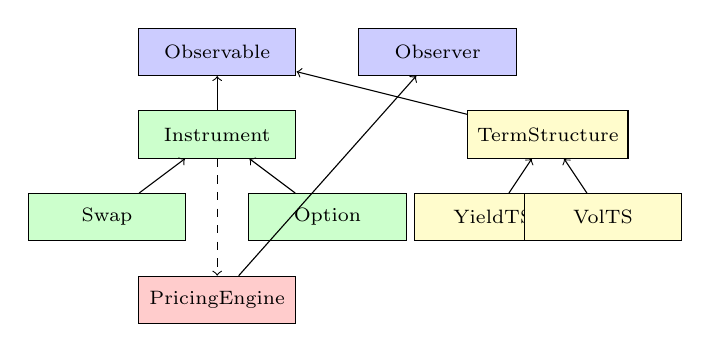
\begin{tikzpicture}[scale=0.7,
    box/.style={rectangle, draw, minimum width=2cm, minimum height=0.6cm, font=\scriptsize}]

    % Observer pattern
    \node[box, fill=blue!20] (obs) at (0,4) {Observable};
    \node[box, fill=blue!20] (obsr) at (4,4) {Observer};

    % Instruments
    \node[box, fill=green!20] (inst) at (0,2.5) {Instrument};
    \node[box, fill=green!20] (swap) at (-2,1) {Swap};
    \node[box, fill=green!20] (opt) at (2,1) {Option};

    % Term structures
    \node[box, fill=yellow!20] (ts) at (6,2.5) {TermStructure};
    \node[box, fill=yellow!20] (yts) at (5,1) {YieldTS};
    \node[box, fill=yellow!20] (vts) at (7,1) {VolTS};

    % Engines
    \node[box, fill=red!20] (eng) at (0,-0.5) {PricingEngine};

    \draw[->] (inst) -- (obs);
    \draw[->] (swap) -- (inst);
    \draw[->] (opt) -- (inst);
    \draw[->] (ts) -- (obs);
    \draw[->] (yts) -- (ts);
    \draw[->] (vts) -- (ts);
    \draw[->] (eng) -- (obsr);
    \draw[dashed,->] (inst) -- (eng);
\end{tikzpicture}
\end{center}

\textbf{Key Patterns:}
\begin{itemize}
    \item Observer/Observable for lazy evaluation
    \item Instruments are priced by Engines
    \item Term structures hold market data
\end{itemize}
\end{frame}

\begin{frame}[fragile]{Date and Calendar Handling}
\begin{lstlisting}[language=Python]
import QuantLib as ql

# Date construction
d1 = ql.Date(15, 8, 2026)           # Day, Month, Year
d2 = ql.Date(15, ql.August, 2026)   # Using enum
d3 = ql.DateParser.parseISO("2026-08-15")

# Date arithmetic
d4 = d1 + ql.Period(3, ql.Months)
d5 = d1 + 30  # Add 30 calendar days

# Calendar operations
cal = ql.UnitedStates(ql.UnitedStates.Settlement)
if cal.isBusinessDay(d1):
    print("Business day")

# Advance by business days
spot = cal.advance(d1, 2, ql.Days)

# Joint calendar (requires both to be open)
joint = ql.JointCalendar(ql.TARGET(),
    ql.UnitedStates(ql.UnitedStates.Settlement),
    ql.JoinHolidays)
\end{lstlisting}
\end{frame}

\begin{frame}[fragile]{Index Classes}
\begin{lstlisting}[language=Python]
# Overnight indices
sofr = ql.Sofr()
estr = ql.Estr()
sonia = ql.Sonia()

# Link to curve
curve_handle = ql.YieldTermStructureHandle(curve)
sofr_with_curve = ql.Sofr(curve_handle)

# Get fixings
fixing_date = ql.Date(10, 8, 2026)
rate = sofr.fixing(fixing_date)

# Add historical fixings (for backward-looking)
ql.IndexManager.instance().clearHistories()
sofr.addFixing(ql.Date(1, 8, 2026), 0.04)
sofr.addFixing(ql.Date(2, 8, 2026), 0.0402)
\end{lstlisting}
\end{frame}

\begin{frame}[fragile]{Yield Curve Construction Details}
\begin{lstlisting}[language=Python]
# Rate helpers
helpers = []

# Deposit helper (for short end)
helpers.append(ql.DepositRateHelper(
    ql.QuoteHandle(ql.SimpleQuote(0.041)),  # Rate
    ql.Period(1, ql.Days),                   # Tenor
    0,                                        # Settlement days
    ql.UnitedStates(ql.UnitedStates.Settlement),
    ql.ModifiedFollowing,                    # Convention
    False,                                   # End of month
    ql.Actual360()                          # Day count
))

# OIS helpers
for tenor, rate in [("1Y", 0.039), ("5Y", 0.037)]:
    helpers.append(ql.OISRateHelper(
        2, ql.Period(tenor),
        ql.QuoteHandle(ql.SimpleQuote(rate)),
        ql.Sofr()
    ))

# Build curve
curve = ql.PiecewiseLogLinearDiscount(today, helpers, ql.Actual365Fixed())
curve.enableExtrapolation()
\end{lstlisting}
\end{frame}

\begin{frame}[fragile]{OvernightIndexedSwap Instrument}
\begin{lstlisting}[language=Python]
# Create OIS swap
schedule = ql.Schedule(
    start_date, end_date,
    ql.Period(ql.Semiannual),          # Payment frequency
    calendar,
    ql.ModifiedFollowing,              # Business day convention
    ql.ModifiedFollowing,
    ql.DateGeneration.Backward,
    False                              # End of month
)

swap = ql.OvernightIndexedSwap(
    ql.Swap.Payer,                     # Type
    100_000_000.0,                     # Notional
    schedule,
    0.04,                              # Fixed rate
    ql.Actual360(),                    # Fixed day count
    ql.Sofr(curve_handle),             # Index
    0.0,                               # Spread on floating
    0,                                 # Payment lag
    ql.ModifiedFollowing,
    calendar
)
\end{lstlisting}
\end{frame}

\begin{frame}[fragile]{Swaption Construction}
\begin{lstlisting}[language=Python]
# Create underlying swap
underlying = ql.VanillaSwap(
    ql.Swap.Payer, notional,
    fixed_schedule, strike, day_count,
    float_schedule, sofr_index, 0.0, day_count
)

# European exercise
expiry = ql.Date(15, 8, 2028)
exercise = ql.EuropeanExercise(expiry)

# Bermudan exercise
call_dates = [ql.Date(15, 8, 2028 + i) for i in range(5)]
exercise = ql.BermudanExercise(call_dates)

# Create swaption
swaption = ql.Swaption(underlying, exercise)

# Set pricing engine
engine = ql.TreeSwaptionEngine(hw_model, 50)
swaption.setPricingEngine(engine)

print(f"NPV: {swaption.NPV():,.2f}")
\end{lstlisting}
\end{frame}

\begin{frame}[fragile]{Hull-White Model Setup}
\begin{lstlisting}[language=Python]
# Create model with fixed parameters
mean_reversion = 0.03
volatility = 0.01
model = ql.HullWhite(curve_handle, mean_reversion, volatility)

# Get model parameters
params = model.params()
print(f"a = {params[0]}, sigma = {params[1]}")

# Create calibration helpers
helpers = []
for expiry, tenor, vol_bp in [("2Y", "8Y", 78), ("5Y", "5Y", 80)]:
    helper = ql.SwaptionHelper(
        ql.Period(expiry), ql.Period(tenor),
        ql.QuoteHandle(ql.SimpleQuote(vol_bp * 1e-4)),
        sofr_index, ql.Period("1Y"), ql.Actual360(),
        ql.Actual360(), curve_handle,
        ql.BlackCalibrationHelper.RelativePriceError,
        ql.nullDouble(), 1.0, ql.Normal
    )
    helper.setPricingEngine(ql.JamshidianSwaptionEngine(model))
    helpers.append(helper)
\end{lstlisting}
\end{frame}

\begin{frame}[fragile]{Model Calibration}
\begin{lstlisting}[language=Python]
# Calibration settings
opt_method = ql.LevenbergMarquardt()
end_criteria = ql.EndCriteria(
    500,    # Max iterations
    100,    # Max stationary
    1e-10,  # Root epsilon
    1e-10,  # Function epsilon
    1e-10   # Gradient epsilon
)

# Which parameters to calibrate
# [True, False] means calibrate a, keep sigma fixed
fixed_params = ql.BoolVector([True, False])

# Run calibration
model.calibrate(
    helpers,        # Calibration instruments
    opt_method,
    end_criteria,
    ql.PositiveConstraint(),  # Parameter constraint
    ql.DoubleVector(),        # Weights
    fixed_params
)

# Check results
print(f"Calibrated sigma: {model.params()[1]:.6f}")
\end{lstlisting}
\end{frame}

\begin{frame}[fragile]{Calibration Diagnostics}
\begin{lstlisting}[language=Python]
# After calibration, check fit quality
for i, helper in enumerate(helpers):
    market_val = helper.marketValue()
    model_val = helper.modelValue()
    error = (model_val - market_val) / market_val

    # Get implied vol
    impl_vol = helper.impliedVolatility(model_val, 1e-6, 100,
                                         1e-6, 2.0)

    print(f"Helper {i}:")
    print(f"  Market: {market_val:.6f}")
    print(f"  Model:  {model_val:.6f}")
    print(f"  Error:  {error*100:.3f}%")
    print(f"  Impl Vol: {impl_vol*10000:.1f}bp")

# Calculate weighted RMS
errors = [(h.modelValue()/h.marketValue() - 1)**2 for h in helpers]
rms = math.sqrt(sum(errors) / len(errors))
print(f"RMS Error: {rms*100:.3f}%")
\end{lstlisting}
\end{frame}

\begin{frame}{QuantLib Limitations for XCCY}
\textbf{Native XCCY Support:}
\begin{itemize}
    \item \texttt{CrossCurrencyBasisSwap} --- exists for vanilla XCCY
    \item \texttt{CrossCurrencyBasisSwapRateHelper} --- for curve building
    \item No native \textbf{callable} XCCY instrument
\end{itemize}

\textbf{Multi-Factor Limitations:}
\begin{itemize}
    \item Tree engines work for 1-2 factors
    \item No native 3-factor joint tree
    \item Would need FD solver on 3D grid (slow)
    \item Monte Carlo is natural choice
\end{itemize}

\textbf{Our Solution:}
\begin{itemize}
    \item Use QuantLib for curves, dates, indices
    \item Custom 3-factor Monte Carlo
    \item LSM for exercise optimization
\end{itemize}
\end{frame}

%%%%%%%%%%%%%%%%%%%%%%%%%%%%%%%%%%%%%%%%%%%%%%%%%%%%%%%%%%%%%%%%%%%%%%%%%%%%%%%%
%% APPENDIX C: MONTE CARLO METHODS (20 slides)
%%%%%%%%%%%%%%%%%%%%%%%%%%%%%%%%%%%%%%%%%%%%%%%%%%%%%%%%%%%%%%%%%%%%%%%%%%%%%%%%

\begin{frame}{}
\begin{center}
\Huge\textbf{Appendix C}\\[1cm]
\Large Monte Carlo Methods\\[0.5cm]
\normalsize Simulation Techniques and Variance Reduction
\end{center}
\end{frame}

\begin{frame}{Monte Carlo Basics}
\begin{block}{Law of Large Numbers}
\[
\frac{1}{N}\sum_{i=1}^{N} f(X_i) \xrightarrow{N\to\infty} \mathbb{E}[f(X)]
\]
\end{block}

\textbf{Standard Error:}
\[
SE = \frac{\sigma}{\sqrt{N}}
\]

\textbf{95\% Confidence Interval:}
\[
\bar{X} \pm 1.96 \times SE
\]

\textbf{Key Properties:}
\begin{itemize}
    \item Error decreases as $O(N^{-1/2})$
    \item Independent of dimension (curse of dimensionality avoided)
    \item Flexible for path-dependent payoffs
\end{itemize}
\end{frame}

\begin{frame}[fragile]{Random Number Generation}
\textbf{NumPy PCG64 Generator:}
\begin{itemize}
    \item Permuted Congruential Generator
    \item Period: $2^{128}$
    \item Excellent statistical properties
    \item Fast and reproducible
\end{itemize}

\textbf{Usage:}
\begin{lstlisting}[language=Python]
import numpy as np

# Create generator with seed
rng = np.random.Generator(np.random.PCG64(1729))

# Generate standard normals
Z = rng.standard_normal((paths, dimensions))
\end{lstlisting}

\textbf{Reproducibility:}
\begin{itemize}
    \item Same seed $\Rightarrow$ same sequence
    \item Critical for debugging and validation
\end{itemize}
\end{frame}

\begin{frame}[fragile]{Variance Reduction: Antithetic Variates}
\begin{block}{Antithetic Sampling}
If $\hat{\theta}_1 = f(Z)$ and $\hat{\theta}_2 = f(-Z)$ are negatively correlated, then:
\[
\text{Var}\left[\frac{\hat{\theta}_1 + \hat{\theta}_2}{2}\right] < \text{Var}[\hat{\theta}_1]
\]
\end{block}

\textbf{Implementation:}
\begin{lstlisting}[language=Python]
def antithetic_normals(rng, paths, dims):
    half = (paths + 1) // 2
    draws = rng.standard_normal((half, dims))
    return np.concatenate([draws, -draws])[:paths]
\end{lstlisting}

\textbf{Benefits:}
\begin{itemize}
    \item Forces mean of normals to be exactly 0
    \item Reduces variance for most payoffs
    \item No additional cost per sample
\end{itemize}
\end{frame}

\begin{frame}{Variance Reduction: Control Variates}
\begin{block}{Control Variate Method}
Use a correlated variable $Y$ with known mean $\mu_Y$:
\[
\hat{\theta}_{CV} = \hat{\theta} - \beta(\bar{Y} - \mu_Y)
\]
\end{block}

\textbf{Optimal $\beta$:}
\[
\beta^* = \frac{\text{Cov}[\hat{\theta}, Y]}{\text{Var}[Y]}
\]

\textbf{Applications in Derivatives:}
\begin{itemize}
    \item Use underlying asset as control
    \item Use European price for Bermudan
    \item Use delta-hedged portfolio
\end{itemize}
\end{frame}

\begin{frame}{Quasi-Monte Carlo (QMC)}
\textbf{Low-Discrepancy Sequences:}
\begin{itemize}
    \item Sobol, Halton, Niederreiter
    \item Fill space more uniformly than random
    \item Error $O(N^{-1})$ vs $O(N^{-1/2})$
\end{itemize}

\textbf{Trade-offs:}
\begin{itemize}
    \item Better for smooth integrands
    \item Dimension-dependent effectiveness
    \item Standard error not directly computable
\end{itemize}

\textbf{Not used in our implementation:}
\begin{itemize}
    \item Standard MC simpler to implement
    \item Antithetic sufficient for our accuracy needs
    \item QMC would be future enhancement
\end{itemize}
\end{frame}

\begin{frame}{Path Generation: Euler vs Exact}
\textbf{Euler Discretization:}
\[
x_{t+\Delta t} = x_t + \mu(x_t)\Delta t + \sigma(x_t)\sqrt{\Delta t}\, Z
\]

\textbf{Exact Simulation (OU process):}
\[
x_{t+h} = x_t e^{-ah} + \sigma\int_0^h e^{-a(h-s)}\,dW_s
\]

\textbf{Our Approach: Exact OU Kernels}
\begin{itemize}
    \item Hull-White factors use exact solution
    \item No discretization bias
    \item Larger time steps possible
    \item Covariance computed exactly
\end{itemize}
\end{frame}

\begin{frame}[fragile]{State Evolution Implementation}
\begin{lstlisting}[language=Python]
@dataclass
class StepTransition:
    matrix: np.ndarray      # Transition matrix A
    offset: np.ndarray      # Deterministic drift b
    covariance_root: np.ndarray  # sqrt(Sigma)

def evolve_state(state, transition, normals):
    """
    x_{t+h} = A * x_t + b + L * Z

    state: (paths, 5) current state
    transition: StepTransition object
    normals: (paths, 5) standard normals

    Returns: (paths, 5) new state
    """
    return (state @ transition.matrix.T
            + transition.offset
            + normals @ transition.covariance_root.T)
\end{lstlisting}
\end{frame}

\begin{frame}{Cash Flow Valuation}
\textbf{For each simulated path:}

\textbf{Fixed Cash Flow:}
\[
PV = \text{Amount} \times e^{-I_{USD}(t_{pay})}
\]

\textbf{Floating Cash Flow (compounded overnight):}
\[
\text{Amount} = N \times \left(e^{I_{EUR}(t_{end}) - I_{EUR}(t_{start}) + \text{basis}} - 1\right)
\]
\[
PV = \text{Amount} \times X_{t_{pay}} \times e^{-I_{USD}(t_{pay})}
\]

\textbf{FX Conversion:} EUR amounts converted at simulated FX rate

\textbf{Notional Exchanges:}
\begin{itemize}
    \item Initial: Net of notionals at spot
    \item Final: Net of notionals at terminal FX
\end{itemize}
\end{frame}

\begin{frame}{LSM: Basis Function Selection}
\textbf{State Variables:} $(x_{USD}, x_{EUR}, \ln X - \ln X_0)$

\textbf{Polynomial Basis (10 functions):}
\[
\phi = (1,\, x,\, y,\, z,\, x^2,\, y^2,\, z^2,\, xy,\, xz,\, yz)
\]

\textbf{Why This Choice?}
\begin{itemize}
    \item Captures main effects (linear terms)
    \item Captures curvature (squared terms)
    \item Captures interactions (cross terms)
    \item Low-dimensional (avoids overfitting)
\end{itemize}

\textbf{Alternatives:}
\begin{itemize}
    \item Laguerre polynomials
    \item Chebyshev polynomials
    \item Neural network approximation
\end{itemize}
\end{frame}

\begin{frame}{LSM: Numerical Stability}
\textbf{Problem: Ill-Conditioned Design Matrix}

When state variables have different scales or are correlated:
\[
\text{cond}(\mathbf{X}^T\mathbf{X}) \gg 1
\]

\textbf{Solutions:}
\begin{enumerate}
    \item \textbf{Standardization:}
    \[
    \tilde{x} = \frac{x - \bar{x}}{\sigma_x}
    \]

    \item \textbf{Ridge Regression:}
    \[
    \boldsymbol{\beta} = (\mathbf{X}^T\mathbf{X} + \lambda\mathbf{I})^{-1}\mathbf{X}^T\mathbf{y}
    \]
\end{enumerate}

\textbf{Our Implementation:}
\begin{itemize}
    \item Standardize state variables
    \item Use \texttt{np.linalg.lstsq} with rcond
    \item Fall back to ridge if cond $>$ 1e10
\end{itemize}
\end{frame}

\begin{frame}{LSM: Two-Pass Why It Matters}
\textbf{Single-Pass Bias:}
\begin{itemize}
    \item Training on same paths as pricing
    \item Exercise decision uses future information
    \item Results in upward bias (too high)
\end{itemize}

\textbf{Two-Pass Solution:}
\begin{enumerate}
    \item \textbf{Training Pass:} Learn policy on paths 1...N
    \item \textbf{Pricing Pass:} Apply policy on paths N+1...2N
\end{enumerate}

\textbf{Properties:}
\begin{itemize}
    \item Pricing paths are independent of training
    \item No look-ahead bias
    \item Result is a \textit{lower bound} on true value
\end{itemize}

\textbf{Why Lower Bound?}
\begin{itemize}
    \item Suboptimal exercise policy
    \item True optimal policy would give higher value
    \item Upper bound requires dual methods
\end{itemize}
\end{frame}

\begin{frame}{Convergence Diagnostics}
\textbf{Standard Error Analysis:}
\[
SE = \frac{\sigma}{\sqrt{N}}
\]

\textbf{Expected Behavior:}
\begin{itemize}
    \item Double paths $\Rightarrow$ SE reduces by $\sqrt{2}$
    \item 10x paths $\Rightarrow$ SE reduces by $\sqrt{10} \approx 3.16$
\end{itemize}

\textbf{Test Protocol:}
\begin{enumerate}
    \item Run with 10K paths, record SE
    \item Run with 40K paths, record SE
    \item Verify ratio $\approx$ 2.0
\end{enumerate}

\textbf{If Ratio is Wrong:}
\begin{itemize}
    \item Implementation bug
    \item Correlation between paths
    \item Numerical instability
\end{itemize}
\end{frame}

%%%%%%%%%%%%%%%%%%%%%%%%%%%%%%%%%%%%%%%%%%%%%%%%%%%%%%%%%%%%%%%%%%%%%%%%%%%%%%%%
%% APPENDIX D: TESTING AND VALIDATION (20 slides)
%%%%%%%%%%%%%%%%%%%%%%%%%%%%%%%%%%%%%%%%%%%%%%%%%%%%%%%%%%%%%%%%%%%%%%%%%%%%%%%%

\begin{frame}{}
\begin{center}
\Huge\textbf{Appendix D}\\[1cm]
\Large Testing and Validation\\[0.5cm]
\normalsize Ensuring Model Correctness
\end{center}
\end{frame}

\begin{frame}{Validation Philosophy}
\begin{block}{Trust, But Verify}
Every model component needs independent validation.
\end{block}

\textbf{Levels of Testing:}
\begin{enumerate}
    \item \textbf{Unit Tests:} Individual functions
    \item \textbf{Integration Tests:} Component interactions
    \item \textbf{Calibration Tests:} Market data fit
    \item \textbf{Model Tests:} Arbitrage conditions
    \item \textbf{Convergence Tests:} Numerical accuracy
    \item \textbf{Boundary Tests:} Edge cases
\end{enumerate}
\end{frame}

\begin{frame}{Martingale Testing: Theory}
\textbf{Under Risk-Neutral Measure:}

Discounted tradeable assets must be martingales:
\[
\mathbb{E}^\mathbb{Q}[e^{-\int_0^T r_s\,ds} \cdot A_T] = A_0
\]

\textbf{Test Assets:}
\begin{enumerate}
    \item \textbf{USD Zero Coupon:} $\mathbb{E}[e^{-\int r^{USD}}] = P^{USD}(0,T)$
    \item \textbf{EUR Zero in USD:} $\mathbb{E}[e^{-\int r^{USD}} X_T] = X_0 P^{EUR}_{eff}(0,T)$
    \item \textbf{EUR Bank Account:} $\mathbb{E}[e^{-\int r^{USD}} X_T e^{\int r^{EUR}}] = X_0$
\end{enumerate}

\textbf{Statistical Test:}
\[
z = \frac{\bar{X}_{MC} - \text{Target}}{SE_{MC}}
\]
Pass if $|z| < 3.5$ (approximate 99.95\% confidence)
\end{frame}

\begin{frame}{Monotonicity Testing}
\textbf{Economic Relationships That Must Hold:}

\begin{itemize}
    \item $\uparrow$ Volatility $\Rightarrow$ $\uparrow$ Option Value
    \item $\uparrow$ Non-call Period $\Rightarrow$ $\downarrow$ Option Value
    \item $\uparrow$ FX Spot (EUR/USD) $\Rightarrow$ $\uparrow$ EUR Leg Value
    \item $\uparrow$ Interest Rates $\Rightarrow$ $\downarrow$ Long Duration Value
\end{itemize}

\textbf{Test Protocol:}
\begin{enumerate}
    \item Price with base parameters
    \item Bump parameter in expected direction
    \item Verify price moves correctly
    \item Allow for MC noise (use confidence bounds)
\end{enumerate}
\end{frame}

\begin{frame}{Structural Bounds}
\textbf{Test 1: Option Value Non-Negative}
\[
V_{callable} \geq V_{non-callable}
\]

\textbf{Test 2: Callable Decomposition}
\[
V_{callable} = V_{non-callable} + V_{option}
\]

\textbf{Test 3: Option Less Than Notional}
\[
V_{option} < \text{Notional}
\]

\textbf{Test 4: Leg Consistency}
\[
V_{USD} + V_{EUR} = V_{non-callable}
\]

(Within Monte Carlo error)
\end{frame}

\begin{frame}[fragile]{Test Implementation Example}
\begin{lstlisting}[language=Python]
class TestStructuralBounds:
    """Test fundamental arbitrage bounds."""

    def test_callable_ge_non_callable(self, base_result):
        """Callable >= Non-callable."""
        callable_npv = base_result["valuation"]["callable_npv"]["mean"]
        non_callable = base_result["valuation"]["non_callable_npv"]["mean"]
        option = base_result["valuation"]["embedded_option_value"]["mean"]

        assert option >= 0, f"Option must be >= 0, got {option:,.2f}"

        # Check decomposition
        recomputed = non_callable + option
        assert abs(callable_npv - recomputed) < 1.0, (
            f"Callable ({callable_npv:,.2f}) != "
            f"Non-callable ({non_callable:,.2f}) + Option ({option:,.2f})"
        )
\end{lstlisting}
\end{frame}

\begin{frame}{Calibration Quality Checks}
\textbf{OIS Curve Bootstrap:}
\begin{itemize}
    \item Each input OIS rate should reprice to $<$0.01bp
    \item Interpolation should be smooth
    \item No negative forward rates
\end{itemize}

\textbf{Swaption Calibration:}
\begin{itemize}
    \item Individual error $<$5\% relative
    \item RMS error $<$5\%
    \item Model parameters in reasonable range
\end{itemize}

\textbf{FX Vol Calibration:}
\begin{itemize}
    \item Each ATM vol within 25bp
    \item Term structure monotonic
    \item Implied sigmas positive
\end{itemize}
\end{frame}

\begin{frame}{Edge Case Testing}
\textbf{Zero Correlation:}
\begin{itemize}
    \item Set all correlations to 0
    \item Model should still work
    \item Results should be sensible
\end{itemize}

\textbf{High Correlation:}
\begin{itemize}
    \item Set correlations to extreme (but valid) values
    \item Check positive semi-definiteness
    \item Verify no numerical issues
\end{itemize}

\textbf{ATM Swap:}
\begin{itemize}
    \item Price with swap at par
    \item Non-callable value near zero
    \item Option value dominates
\end{itemize}
\end{frame}

\begin{frame}{Regression Testing}
\textbf{Golden Reference:}
\begin{itemize}
    \item Store results from validated run
    \item Compare new runs against reference
    \item Flag any deviations
\end{itemize}

\textbf{What to Compare:}
\begin{itemize}
    \item Calibrated parameters
    \item NPV values (within MC noise)
    \item Exercise probabilities
    \item Greeks (if computed)
\end{itemize}

\textbf{When to Update Reference:}
\begin{itemize}
    \item Bug fixes that change results
    \item Model enhancements
    \item After thorough validation
\end{itemize}
\end{frame}

\begin{frame}{Performance Testing}
\textbf{Benchmarks:}
\begin{itemize}
    \item Full pricing: $<$15 seconds
    \item 30,000 paths, 10Y horizon
    \item MacBook M1/M2 baseline
\end{itemize}

\textbf{Bottlenecks:}
\begin{enumerate}
    \item Path simulation (main loop)
    \item Cash flow accumulation
    \item Regression (matrix operations)
\end{enumerate}

\textbf{Optimization Strategies:}
\begin{itemize}
    \item Vectorize all operations
    \item Minimize memory allocation
    \item Use efficient BLAS (via NumPy)
    \item Consider chunking for large N
\end{itemize}
\end{frame}

%%%%%%%%%%%%%%%%%%%%%%%%%%%%%%%%%%%%%%%%%%%%%%%%%%%%%%%%%%%%%%%%%%%%%%%%%%%%%%%%
%% APPENDIX E: PRACTICAL CONSIDERATIONS (20 slides)
%%%%%%%%%%%%%%%%%%%%%%%%%%%%%%%%%%%%%%%%%%%%%%%%%%%%%%%%%%%%%%%%%%%%%%%%%%%%%%%%

\begin{frame}{}
\begin{center}
\Huge\textbf{Appendix E}\\[1cm]
\Large Practical Considerations\\[0.5cm]
\normalsize Real-World Deployment Challenges
\end{center}
\end{frame}

\begin{frame}{Market Data Challenges}
\textbf{Data Sources:}
\begin{itemize}
    \item Bloomberg, Reuters
    \item Exchange feeds
    \item Broker quotes
\end{itemize}

\textbf{Data Quality Issues:}
\begin{itemize}
    \item Stale quotes
    \item Bid/ask spreads
    \item Missing data points
    \item Timezone differences
\end{itemize}

\textbf{Our Approach:}
\begin{itemize}
    \item JSON input files
    \item Placeholder/illustrative data
    \item Clear ``REPLACE'' markers
    \item Schema validation
\end{itemize}
\end{frame}

\begin{frame}{Collateral and Funding}
\textbf{CSA (Credit Support Annex):}
\begin{itemize}
    \item Determines collateral posting rules
    \item Affects discount curve choice
    \item USD CSA $\Rightarrow$ SOFR discounting
\end{itemize}

\textbf{Cross-Currency Collateral:}
\begin{itemize}
    \item EUR deal, USD collateral
    \item Creates ``effective'' EUR curve
    \item Different from native EUR curve
\end{itemize}

\textbf{Our Implementation:}
\begin{itemize}
    \item Build EUR effective curve from FX forwards
    \item Discount EUR flows at effective rate
    \item Maintain forecast/discount separation
\end{itemize}
\end{frame}

\begin{frame}{Model Risk Management}
\textbf{Key Risks:}
\begin{itemize}
    \item Calibration failure
    \item Parameter instability
    \item Numerical errors
    \item Assumption violations
\end{itemize}

\textbf{Mitigations:}
\begin{itemize}
    \item Tolerance thresholds
    \item Calibration acceptance flags
    \item Martingale diagnostics
    \item Limitation documentation
\end{itemize}

\textbf{Documentation:}
\begin{itemize}
    \item Model specification
    \item Validation report
    \item Known limitations
    \item Appropriate use guidance
\end{itemize}
\end{frame}

\begin{frame}{Greeks and Risk}
\textbf{Bump-and-Revalue:}
\begin{itemize}
    \item Shift input, reprice, compute difference
    \item Simple but expensive
    \item Need common random numbers
\end{itemize}

\textbf{Key Greeks:}
\begin{itemize}
    \item \textbf{Delta:} $\partial V / \partial \text{rates}$
    \item \textbf{Vega:} $\partial V / \partial \text{vol}$
    \item \textbf{FX Delta:} $\partial V / \partial X$
    \item \textbf{Correlation:} $\partial V / \partial \rho$
\end{itemize}

\textbf{Not Implemented Yet:}
\begin{itemize}
    \item Pathwise derivatives
    \item Likelihood ratio method
    \item AAD (automatic differentiation)
\end{itemize}
\end{frame}

\begin{frame}{Performance Optimization}
\textbf{Current Performance:}
\begin{itemize}
    \item 30K paths: $\sim$10 seconds
    \item 100K paths: $\sim$30 seconds
    \item Acceptable for research
\end{itemize}

\textbf{Potential Improvements:}
\begin{enumerate}
    \item \textbf{Numba JIT:} Compile hot loops
    \item \textbf{CuPy:} GPU acceleration
    \item \textbf{Cython:} C extensions
    \item \textbf{C++ Port:} Full rewrite
\end{enumerate}

\textbf{Trade-offs:}
\begin{itemize}
    \item Development time vs runtime
    \item Maintainability
    \item Debugging complexity
\end{itemize}
\end{frame}

\begin{frame}{Production Readiness Checklist}
\textbf{Before Production Use:}
\begin{enumerate}
    \item[$\square$] Independent model review
    \item[$\square$] Dual/upper bound implementation
    \item[$\square$] Full market data integration
    \item[$\square$] Greeks computation
    \item[$\square$] Audit trail
    \item[$\square$] Error handling review
    \item[$\square$] Performance testing
    \item[$\square$] Security audit
    \item[$\square$] Documentation complete
    \item[$\square$] Regulatory approval
\end{enumerate}

\textbf{Current Status:} Research/educational use only
\end{frame}

\begin{frame}{Lessons Learned}
\begin{enumerate}
    \item \textbf{Start Simple:} Build vanilla first, then exotic

    \item \textbf{Validate Early:} Test each component before integration

    \item \textbf{Document Assumptions:} Future you will forget

    \item \textbf{Use QuantLib:} Don't reinvent dates, calendars, curves

    \item \textbf{Vectorize:} NumPy is your friend

    \item \textbf{Test Extensively:} Martingales, bounds, convergence

    \item \textbf{Accept Limitations:} No model is perfect
\end{enumerate}
\end{frame}

\begin{frame}{Resources and References}
\textbf{Books:}
\begin{itemize}
    \item Brigo \& Mercurio: ``Interest Rate Models''
    \item Glasserman: ``Monte Carlo Methods in Financial Engineering''
    \item Longstaff \& Schwartz (2001): LSM Paper
\end{itemize}

\textbf{QuantLib:}
\begin{itemize}
    \item \url{https://www.quantlib.org}
    \item \url{https://github.com/lballabio/QuantLib}
    \item \url{https://quantlib-python-docs.readthedocs.io}
\end{itemize}

\textbf{This Project:}
\begin{itemize}
    \item Repository: \texttt{tgir\_quantlib\_tools}
    \item Model ID: \texttt{HW1F\_USD\_HW1F\_EUR\_BSFX\_LSM\_V1}
\end{itemize}
\end{frame}

\begin{frame}{}
\begin{center}
\Huge\textbf{Appendix F}\\[1cm]
\Large Collaborative AI Development\\[0.5cm]
\normalsize Human + Codex + Claude + Tools
\end{center}
\end{frame}

%%%%%%%%%%%%%%%%%%%%%%%%%%%%%%%%%%%%%%%%%%%%%%%%%%%%%%%%%%%%%%%%%%%%%%%%%%%%%%%%
%% APPENDIX F: COLLABORATIVE AI DEVELOPMENT
%%%%%%%%%%%%%%%%%%%%%%%%%%%%%%%%%%%%%%%%%%%%%%%%%%%%%%%%%%%%%%%%%%%%%%%%%%%%%%%%

\begin{frame}{The Collaborative Development Model}
\textbf{This project demonstrates a new development paradigm:}

\begin{center}
\fbox{\parbox{0.85\textwidth}{\centering
\textbf{Human Domain Expert} (orchestrator)\\
$\downarrow$\\
\textbf{Codex} (specs, core programming, tests)\\
$\downarrow$\\
\textbf{Claude} (review, validation framework, extensions)\\
$\downarrow$\\
\textbf{Production System} (Mac + DigitalOcean)
}}
\end{center}

\vspace{0.5cm}
\textbf{Key Insight:}\\
The collaborative methodology is \textbf{as significant as the callable XCCY pricer itself}

\textbf{Reproducible Pattern:} Same workflow can build other complex pricers
\end{frame}

\begin{frame}{Division of Labor: Two AI Agents}
\begin{table}
\centering
\small
\begin{tabular}{p{3cm}p{4cm}p{4cm}}
\toprule
& \textbf{Codex (OpenAI)} & \textbf{Claude (Anthropic)} \\
\midrule
\textbf{Primary Role} & Core development & Review \& validation \\
\midrule
\textbf{Specs} & Wrote formal specifications & Reviewed for completeness \\
\textbf{Implementation} & Built Monte Carlo engine & Reviewed for correctness \\
\textbf{Tests} & Created initial test suite & Built validation framework \\
\textbf{Extensions} & --- & Extended with regression tests \\
\bottomrule
\end{tabular}
\end{table}

\textbf{Human Role:}
\begin{itemize}
    \item Provided domain expertise (financial mathematics)
    \item Orchestrated agent collaboration
    \item Final validation against theory
    \item Verified with Stack Overflow guidance
\end{itemize}
\end{frame}

\begin{frame}{Codex: Ground-Up Development}
\textbf{What Codex Built from Human Guidance:}

\begin{enumerate}
    \item \textbf{Rigorous Specifications:}
    \begin{itemize}
        \item Mathematical model documentation (LaTeX)
        \item API contracts with type hints
        \item JSON schemas for market data and trades
    \end{itemize}

    \item \textbf{Core Implementation:}
    \begin{itemize}
        \item Three-factor Monte Carlo (1,400+ lines)
        \item Longstaff-Schwartz regression
        \item SOFR/ESTR curve bootstrapping
        \item QuantLib integration layer
    \end{itemize}

    \item \textbf{Initial Test Suite:}
    \begin{itemize}
        \item Unit tests for each component
        \item Integration tests for pricing
        \item Smoke tests for API
    \end{itemize}
\end{enumerate}

\textbf{Human provided:} Math formulas, market conventions, QuantLib patterns
\end{frame}

\begin{frame}{Claude: Review and Validation Framework}
\textbf{Claude's Key Contributions:}

\begin{enumerate}
    \item \textbf{Code Review:}
    \begin{itemize}
        \item Reviewed all Codex implementations
        \item Identified numerical stability issues
        \item Suggested vectorization optimizations
    \end{itemize}

    \item \textbf{Validation Framework (Critical):}
    \begin{itemize}
        \item Martingale test infrastructure
        \item Structural bounds verification
        \item Monotonicity checking
        \item Convergence analysis
    \end{itemize}

    \item \textbf{Extensions for Regression:}
    \begin{itemize}
        \item Built tests to catch future changes
        \item Automated validation on every commit
        \item Documentation and lecture generation
    \end{itemize}
\end{enumerate}

\textbf{Result:} 20 automated tests that provide confidence in correctness
\end{frame}

\begin{frame}{The Full Technology Ecosystem}
\begin{table}
\centering
\small
\begin{tabular}{lll}
\toprule
\textbf{Layer} & \textbf{Component} & \textbf{Role} \\
\midrule
\multirow{2}{*}{Infrastructure} & Mac (local) & Development environment \\
 & DigitalOcean & Production hosting \\
\midrule
\multirow{3}{*}{AI Agents} & Codex (OpenAI) & Specs, core dev, tests \\
 & Claude (Anthropic) & Review, validation, docs \\
 & GitHub Copilot & Inline VS Code assistance \\
\midrule
\multirow{2}{*}{Libraries} & QuantLib (C++) & Curves, calibration \\
 & Python/NumPy & Simulation, Flask \\
\midrule
Resources & Stack Overflow & Guidance verification \\
\bottomrule
\end{tabular}
\end{table}

\textbf{Cohesion:} All components integrated in unified workflow
\end{frame}

\begin{frame}{Integration Boundaries: Proposed REST + Implemented MCP}
\textbf{Two Ways to Access the Pricer:}

\begin{table}
\centering
\small
\begin{tabular}{lll}
\toprule
\textbf{Interface} & \textbf{Use Case} & \textbf{Protocol} \\
\midrule
REST contract & Future trading system integration & HTTPS + JSON \\
 & (C++ clients, batch jobs) & Proposed /api/v1/ endpoints \\
\midrule
MCP Server & LLM integration & JSON-RPC \\
 & (Claude, GPT can call pricer) & stdio or HTTP \\
\bottomrule
\end{tabular}
\end{table}

\textbf{Specified REST Endpoints (not yet implemented):}
\begin{itemize}
    \item \texttt{POST /api/v1/callable-xccy/price} --- Sync pricing
    \item \texttt{POST /api/v1/callable-xccy/jobs} --- Async job submission
    \item \texttt{GET /api/v1/engine} --- Schema and limits
\end{itemize}

\textbf{Key Principle:} No QuantLib/Python types cross API boundary
\end{frame}

\begin{frame}{Collaborative Workflow Diagram}
\begin{center}
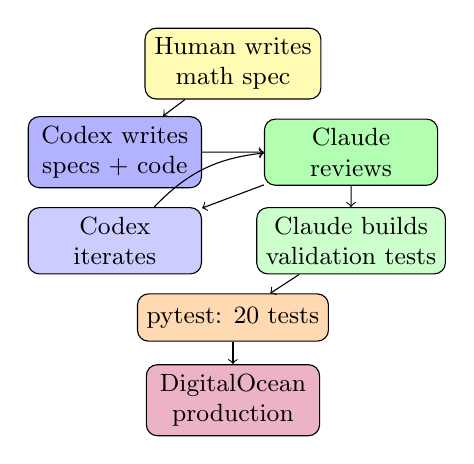
\begin{tikzpicture}[scale=0.75,
    box/.style={rectangle, draw, rounded corners, minimum width=2.2cm, minimum height=0.6cm, align=center, font=\small}]

    \node[box, fill=yellow!30] (human) at (0,4) {Human writes\\math spec};
    \node[box, fill=blue!30] (codex1) at (-2,2.5) {Codex writes\\specs + code};
    \node[box, fill=green!30] (claude1) at (2,2.5) {Claude\\reviews};
    \node[box, fill=blue!20] (codex2) at (-2,1) {Codex\\iterates};
    \node[box, fill=green!20] (claude2) at (2,1) {Claude builds\\validation tests};
    \node[box, fill=orange!30] (pytest) at (0,-0.3) {pytest: 20 tests};
    \node[box, fill=purple!30] (deploy) at (0,-1.7) {DigitalOcean\\production};

    \draw[->] (human) -- (codex1);
    \draw[->] (codex1) -- (claude1);
    \draw[->] (claude1) -- (codex2);
    \draw[->] (claude1) -- (claude2);
    \draw[->] (codex2) to[bend left=20] (claude1);
    \draw[->] (claude2) -- (pytest);
    \draw[->] (pytest) -- (deploy);
\end{tikzpicture}
\end{center}

\textbf{Iteration:} Multiple cycles until all 20 tests pass
\end{frame}

\begin{frame}{Zero-Intervention Automation Pipeline}
\textbf{A Hobby Project with Production-Grade Rigor:}

One prompt triggers the \textbf{entire pipeline} --- no human intervention:

\begin{enumerate}
    \item \textcolor{blue!70}{\textbf{Coding}} --- AI implements from specs
    \item \textcolor{orange!70}{\textbf{Regression Testing}} --- pytest runs 20+ tests locally
    \item \textcolor{purple!70}{\textbf{Browser UI Testing}} --- Playwright validates Flask UI
    \item \textcolor{green!70}{\textbf{Documentation}} --- LaTeX auto-updated
    \item \textcolor{cyan!70}{\textbf{Deploy to DigitalOcean}} --- SSH + Git + systemd
    \item \textcolor{orange!70}{\textbf{Production Regression}} --- Tests on live server
    \item \textcolor{red!70}{\textbf{Telegram Notification}} --- ``Done!''
\end{enumerate}

\vspace{0.2cm}
\begin{center}
\fbox{\parbox{0.85\textwidth}{
\textbf{Key Insight:} \$7/month hobby project built with the same rigor as top tech company production systems.
}}
\end{center}
\end{frame}

\begin{frame}{QuantLib Extension Strategy}
\textbf{QuantLib's Limitations:}
\begin{itemize}
    \item No native callable XCCY support
    \item Limited multi-currency Monte Carlo
    \item No built-in LSM for cross-currency
\end{itemize}

\textbf{How We Extended It (Collaboratively):}
\begin{enumerate}
    \item \textbf{Human:} Defined what QuantLib provides vs what's needed
    \item \textbf{Codex:} Wrote custom Monte Carlo using QuantLib curves
    \item \textbf{Claude:} Verified QuantLib API usage against docs
    \item \textbf{Stack Overflow:} Confirmed edge cases and patterns
\end{enumerate}

\textbf{Result:}
\begin{itemize}
    \item Use QuantLib for: curves, dates, calendars, basic calibration
    \item Custom code for: multi-factor MC, LSM, XCCY cashflows
    \item 1,400+ lines of rigorous extensions
\end{itemize}
\end{frame}

\begin{frame}[fragile]{DigitalOcean Deployment: Detailed Steps}
\textbf{1. Droplet Creation (DigitalOcean Console):}
\begin{itemize}
    \item Region: NYC3 or SFO3 for US users
    \item Image: Ubuntu 22.04 LTS
    \item Plan: Basic \$7/month (2GB RAM, 1 vCPU) --- hobby-friendly!
    \item Authentication: SSH key (not password)
\end{itemize}

\textbf{2. Initial Server Setup:}
\begin{verbatim}
ssh root@your-droplet-ip
apt update && apt upgrade -y
adduser deploy
usermod -aG sudo deploy
\end{verbatim}

\textbf{3. Application Deployment:}
\begin{verbatim}
cd /opt && git clone <repo>
python3 -m venv .venv
.venv/bin/pip install -r requirements.txt
cp deploy/systemd/*.template /etc/systemd/system/
systemctl enable --now tgir-quantlib-tools
\end{verbatim}
\end{frame}

\begin{frame}[fragile]{DigitalOcean: SSL and Apache Configuration}
\textbf{Apache Setup:}
\begin{verbatim}
apt install apache2
a2enmod proxy proxy_http ssl rewrite
cp deploy/apache/*.template /etc/apache2/sites-available/
a2ensite tgir-quantlib-tools
systemctl reload apache2
\end{verbatim}

\textbf{SSL with Certbot:}
\begin{verbatim}
apt install certbot python3-certbot-apache
certbot --apache -d your-domain.com
\end{verbatim}

\textbf{Firewall:}
\begin{verbatim}
ufw allow 22/tcp
ufw allow 80/tcp
ufw allow 443/tcp
ufw enable
\end{verbatim}

\textbf{Result:} HTTPS-secured Flask app at \texttt{https://your-domain.com}
\end{frame}

\begin{frame}{Why Codex + Claude Collaboration Works}
\textbf{Complementary Strengths:}
\begin{itemize}
    \item \textbf{Codex:} Excellent at ground-up implementation from specs
    \item \textbf{Claude:} Excellent at review, validation, extension
    \item \textbf{Human:} Domain expertise, orchestration, final judgment
\end{itemize}

\textbf{Error Detection:}
\begin{itemize}
    \item Claude catches bugs in Codex's implementations
    \item Codex fixes issues Claude identifies
    \item Neither alone would produce same quality
\end{itemize}

\textbf{Stack Overflow Role:}
\begin{itemize}
    \item AI can hallucinate APIs that don't exist
    \item Human experts catch edge cases
    \item Community validates approaches
\end{itemize}

\textbf{Key Lesson:}\\[0.2cm]
\fbox{\parbox{0.85\textwidth}{\centering Two AI agents + human domain expert\\produces better results than any single agent}}
\end{frame}

\begin{frame}{The Methodology IS the Innovation}
\textbf{This project delivers TWO things:}

\begin{enumerate}
    \item \textbf{Callable XCCY Pricer:}
    \begin{itemize}
        \item Three-factor Monte Carlo
        \item Longstaff-Schwartz optimization
        \item 20 validation tests
        \item Production deployment
    \end{itemize}

    \item \textbf{Collaborative Development Methodology:}
    \begin{itemize}
        \item Human $\to$ Codex (specs, implementation)
        \item Codex $\to$ Claude (review, validation)
        \item Claude $\to$ Regression tests (future-proofing)
        \item Full ecosystem: Mac + DigitalOcean + QuantLib + Python
    \end{itemize}
\end{enumerate}

\vspace{0.3cm}
\textbf{The methodology is reusable for other complex pricers}

\fbox{\parbox{0.85\textwidth}{\centering The collaborative workflow is as valuable as the callable XCCY pricer itself}}
\end{frame}

\begin{frame}{Reusable Human-Agent Development Pattern}
\begin{center}
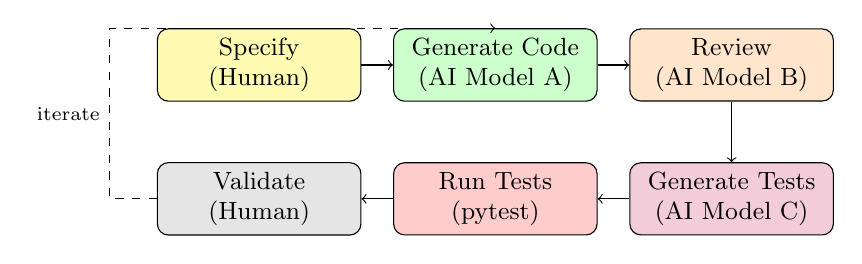
\begin{tikzpicture}[
    box/.style={rectangle, draw, rounded corners, text width=2.35cm, minimum height=0.9cm, align=center, font=\small}]
    \node[box, fill=yellow!30] (spec) at (-3,2.4) {Specify\\(Human)};
    \node[box, fill=green!20] (gen) at (0,2.4) {Generate Code\\(AI Model A)};
    \node[box, fill=orange!20] (review) at (3,2.4) {Review\\(AI Model B)};
    \node[box, fill=purple!20] (test) at (3,0.7) {Generate Tests\\(AI Model C)};
    \node[box, fill=red!20] (run) at (0,0.7) {Run Tests\\(pytest)};
    \node[box, fill=gray!20] (valid) at (-3,0.7) {Validate\\(Human)};

    \draw[->] (spec) -- (gen);
    \draw[->] (gen) -- (review);
    \draw[->] (review) -- (test);
    \draw[->] (test) -- (run);
    \draw[->] (run) -- (valid);
    \draw[->, dashed] (valid.west) -- ++(-0.6,0) |- node[pos=0.25,left,font=\scriptsize] {iterate} (gen.north);
\end{tikzpicture}
\end{center}

\textbf{Key Principle:}\\[0.3cm]
\fbox{\parbox{0.85\textwidth}{\centering Human provides specifications and validation\\AI accelerates implementation and review}}
\end{frame}

\begin{frame}{}
\begin{center}
\Huge\textbf{End of Supplementary Material}\\[2cm]
\Large Return to Main Presentation
\end{center}
\end{frame}

\end{document}

% Or compile separately

\documentclass[aspectratio=169,11pt]{beamer}
\usepackage[T1]{fontenc}
\usepackage[utf8]{inputenc}
\usepackage{lmodern}
\usepackage{mastering_ir_derivatives_beamer_1.0}
\usepackage{booktabs}
\usepackage{array}
\usepackage{listings}

% Retain the supplied visual system without changing the authored slide count.
\beamerdefaultoverlayspecification{<*>}
\AtBeginSection[]{}
\AtBeginSubsection[]{}

\hypersetup{
    colorlinks=true,
    linkcolor=blue,
    urlcolor=blue
}

\lstset{
    basicstyle=\ttfamily\scriptsize,
    breaklines=true,
    columns=fullflexible
}

\newcommand{\product}{TGIR QuantLib Tools}
\newcommand{\code}[1]{\texttt{#1}}
\newcommand{\docdate}{2026-04-06}


\usepackage[utf8]{inputenc}
\usepackage{amsmath,amssymb}
\usepackage{booktabs}
\usepackage{multirow}
\usepackage{listings}
\usepackage{tikz}
\usepackage{xcolor}

\lstset{
    language=Python,
    basicstyle=\ttfamily\scriptsize,
    keywordstyle=\color{blue}\bfseries,
    commentstyle=\color{green!50!black},
    stringstyle=\color{red},
    showstringspaces=false,
    breaklines=true,
    frame=single,
    backgroundcolor=\color{gray!10}
}

\title[Supplementary Content]{\textbf{QuantLib Derivatives Pricing}\\Supplementary Technical Slides}
\author{Quantitative Analytics Team}
\date{August 2026}

\begin{document}

%%%%%%%%%%%%%%%%%%%%%%%%%%%%%%%%%%%%%%%%%%%%%%%%%%%%%%%%%%%%%%%%%%%%%%%%%%%%%%%%
%% APPENDIX A: MATHEMATICAL FOUNDATIONS (20 slides)
%%%%%%%%%%%%%%%%%%%%%%%%%%%%%%%%%%%%%%%%%%%%%%%%%%%%%%%%%%%%%%%%%%%%%%%%%%%%%%%%

\begin{frame}
\titlepage
\end{frame}

\begin{frame}{}
\begin{center}
\Huge\textbf{Appendix A}\\[1cm]
\Large Mathematical Foundations\\[0.5cm]
\normalsize Stochastic Calculus Essentials
\end{center}
\end{frame}

\begin{frame}{Brownian Motion: Definition}
\begin{block}{Standard Brownian Motion $W_t$}
A stochastic process with:
\begin{enumerate}
    \item $W_0 = 0$
    \item Independent increments: $W_t - W_s \perp W_s - W_u$ for $t > s > u$
    \item Normally distributed: $W_t - W_s \sim N(0, t-s)$
    \item Continuous paths
\end{enumerate}
\end{block}

\textbf{Key Properties:}
\begin{itemize}
    \item $\mathbb{E}[W_t] = 0$
    \item $\text{Var}[W_t] = t$
    \item $\mathbb{E}[W_t W_s] = \min(t, s)$
    \item Paths are nowhere differentiable
\end{itemize}
\end{frame}

\begin{frame}{Itô's Lemma}
\begin{block}{Itô's Formula}
For $f(t, X_t)$ where $dX_t = \mu\,dt + \sigma\,dW_t$:
\[
df = \frac{\partial f}{\partial t}dt + \frac{\partial f}{\partial x}dX_t + \frac{1}{2}\frac{\partial^2 f}{\partial x^2}\sigma^2 dt
\]
\end{block}

\textbf{Example: Geometric Brownian Motion}

Let $S_t$ follow $dS_t = \mu S_t\,dt + \sigma S_t\,dW_t$. Apply Itô to $f(S) = \ln S$:
\[
d\ln S = \frac{1}{S}dS - \frac{1}{2}\frac{1}{S^2}\sigma^2 S^2 dt = \left(\mu - \frac{\sigma^2}{2}\right)dt + \sigma\,dW_t
\]

Therefore: $S_T = S_0 \exp\left[(\mu - \frac{\sigma^2}{2})T + \sigma W_T\right]$
\end{frame}

\begin{frame}{Risk-Neutral Pricing}
\begin{block}{Fundamental Theorem of Asset Pricing}
No-arbitrage $\Leftrightarrow$ Exists a probability measure $\mathbb{Q}$ such that discounted asset prices are martingales.
\end{block}

\textbf{Pricing Formula:}
\[
V_0 = \mathbb{E}^\mathbb{Q}\left[e^{-\int_0^T r_s\,ds} \cdot \text{Payoff}_T\right]
\]

\textbf{Change of Measure (Girsanov):}
\begin{itemize}
    \item Under $\mathbb{P}$: $dS = \mu S\,dt + \sigma S\,dW^\mathbb{P}$
    \item Under $\mathbb{Q}$: $dS = r S\,dt + \sigma S\,dW^\mathbb{Q}$
    \item $dW^\mathbb{Q} = dW^\mathbb{P} + \frac{\mu - r}{\sigma}dt$
\end{itemize}
\end{frame}

\begin{frame}{Ornstein-Uhlenbeck Process}
\begin{block}{OU Process}
\[
dx_t = -a x_t\,dt + \sigma\,dW_t
\]
\end{block}

\textbf{Solution:}
\[
x_t = x_0 e^{-at} + \sigma \int_0^t e^{-a(t-s)}\,dW_s
\]

\textbf{Properties:}
\begin{itemize}
    \item Mean: $\mathbb{E}[x_t] = x_0 e^{-at}$
    \item Variance: $\text{Var}[x_t] = \frac{\sigma^2}{2a}(1 - e^{-2at})$
    \item Stationary distribution: $N(0, \frac{\sigma^2}{2a})$
    \item Auto-correlation: $\text{Corr}(x_t, x_s) = e^{-a|t-s|}$
\end{itemize}

\textbf{Hull-White:} Add time-dependent mean $\theta(t)$
\end{frame}

\begin{frame}{Affine Term Structure Models}
\begin{block}{Affine Property}
Discount bond prices have the form:
\[
P(t, T) = e^{A(t,T) - B(t,T) r_t}
\]
\end{block}

\textbf{For Hull-White:}
\[
B(t, T) = \frac{1 - e^{-a(T-t)}}{a}
\]
\[
A(t, T) = \int_t^T \theta(s) B(s, T)\,ds - \frac{\sigma^2}{2}\int_t^T B(s, T)^2\,ds
\]

\textbf{Implications:}
\begin{itemize}
    \item Analytical bond and swaption prices
    \item Efficient calibration
    \item Foundation for tree methods
\end{itemize}
\end{frame}

\begin{frame}{Multi-Factor Models: Correlated Brownians}
\textbf{Correlated Brownian Motions:}

Given correlation matrix $\mathbf{R}$, generate correlated increments:
\[
\begin{pmatrix} dW_1 \\ dW_2 \\ dW_3 \end{pmatrix} = \mathbf{L} \cdot \begin{pmatrix} dZ_1 \\ dZ_2 \\ dZ_3 \end{pmatrix}
\]

Where $\mathbf{L}$ is the Cholesky decomposition: $\mathbf{R} = \mathbf{L}\mathbf{L}^T$

\textbf{Example:} $\rho_{12} = 0.25$, $\rho_{13} = -0.15$, $\rho_{23} = -0.30$

\[
\mathbf{L} = \begin{pmatrix}
1 & 0 & 0 \\
0.25 & 0.968 & 0 \\
-0.15 & -0.271 & 0.951
\end{pmatrix}
\]
\end{frame}

\begin{frame}{Variance Calculation for Joint Processes}
\textbf{For state $\mathbf{x}_t$:}
\[
\text{Cov}[\mathbf{x}_{t+h}, \mathbf{x}_{t+h}] = \int_0^h \mathbf{K}(s) \cdot \mathbf{R} \cdot \mathbf{K}(s)^T\,ds
\]

Where $\mathbf{K}(s)$ is the kernel matrix mapping Brownians to state.

\textbf{Numerical Integration:}
\[
\int_0^h f(s)\,ds \approx \frac{h}{2}\sum_{i=1}^{n} w_i f\left(\frac{h}{2}(x_i + 1)\right)
\]

Using Gauss-Legendre nodes $x_i$ and weights $w_i$.

\textbf{Our Implementation:} 16-point Gauss-Legendre quadrature
\end{frame}

\begin{frame}{Change of Numéraire}
\begin{block}{Numéraire Change}
When changing from numéraire $N_1$ to $N_2$:
\[
\frac{d\mathbb{Q}^{N_2}}{d\mathbb{Q}^{N_1}}\bigg|_{\mathcal{F}_T} = \frac{N_2(T) / N_2(0)}{N_1(T) / N_1(0)}
\]
\end{block}

\textbf{FX Pricing Application:}

Under USD money-market measure:
\begin{itemize}
    \item USD bank account is numéraire
    \item EUR rates get quanto adjustment
    \item FX drift includes rate differential
\end{itemize}

\[
d\ln X = (r^{USD} - r^{EUR} - \tfrac{1}{2}\sigma_X^2)\,dt + \sigma_X\,dW_X
\]
\end{frame}

\begin{frame}{Quanto Adjustment Derivation}
\textbf{Setting:} Price a EUR asset $S^{EUR}$ from USD perspective

\textbf{Under EUR measure:}
\[
dS^{EUR} = r^{EUR} S^{EUR}\,dt + \sigma_S S^{EUR}\,dW_S^{EUR}
\]

\textbf{Converting to USD measure:}
\[
dS^{EUR} = (r^{EUR} - \rho_{S,X}\sigma_S\sigma_X) S^{EUR}\,dt + \sigma_S S^{EUR}\,dW_S^{USD}
\]

\textbf{Intuition:}
\begin{itemize}
    \item If $\rho_{S,X} > 0$: Asset rises when EUR appreciates
    \item Extra expected USD return from FX
    \item Must subtract to stay risk-neutral
\end{itemize}
\end{frame}

%%%%%%%%%%%%%%%%%%%%%%%%%%%%%%%%%%%%%%%%%%%%%%%%%%%%%%%%%%%%%%%%%%%%%%%%%%%%%%%%
%% APPENDIX B: QUANTLIB DEEP DIVE (20 slides)
%%%%%%%%%%%%%%%%%%%%%%%%%%%%%%%%%%%%%%%%%%%%%%%%%%%%%%%%%%%%%%%%%%%%%%%%%%%%%%%%

\begin{frame}{}
\begin{center}
\Huge\textbf{Appendix B}\\[1cm]
\Large QuantLib Deep Dive\\[0.5cm]
\normalsize Internal Architecture and APIs
\end{center}
\end{frame}

\begin{frame}{QuantLib Class Hierarchy}
\begin{center}
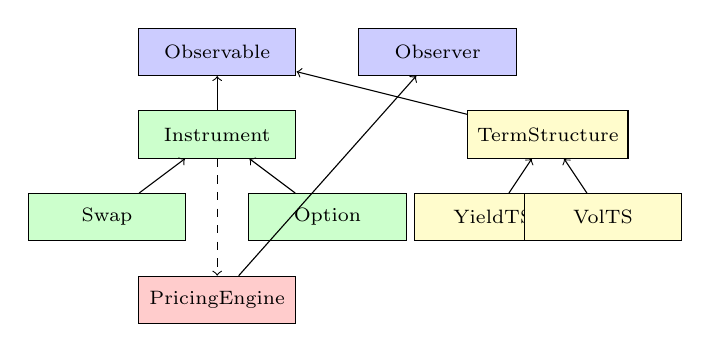
\begin{tikzpicture}[scale=0.7,
    box/.style={rectangle, draw, minimum width=2cm, minimum height=0.6cm, font=\scriptsize}]

    % Observer pattern
    \node[box, fill=blue!20] (obs) at (0,4) {Observable};
    \node[box, fill=blue!20] (obsr) at (4,4) {Observer};

    % Instruments
    \node[box, fill=green!20] (inst) at (0,2.5) {Instrument};
    \node[box, fill=green!20] (swap) at (-2,1) {Swap};
    \node[box, fill=green!20] (opt) at (2,1) {Option};

    % Term structures
    \node[box, fill=yellow!20] (ts) at (6,2.5) {TermStructure};
    \node[box, fill=yellow!20] (yts) at (5,1) {YieldTS};
    \node[box, fill=yellow!20] (vts) at (7,1) {VolTS};

    % Engines
    \node[box, fill=red!20] (eng) at (0,-0.5) {PricingEngine};

    \draw[->] (inst) -- (obs);
    \draw[->] (swap) -- (inst);
    \draw[->] (opt) -- (inst);
    \draw[->] (ts) -- (obs);
    \draw[->] (yts) -- (ts);
    \draw[->] (vts) -- (ts);
    \draw[->] (eng) -- (obsr);
    \draw[dashed,->] (inst) -- (eng);
\end{tikzpicture}
\end{center}

\textbf{Key Patterns:}
\begin{itemize}
    \item Observer/Observable for lazy evaluation
    \item Instruments are priced by Engines
    \item Term structures hold market data
\end{itemize}
\end{frame}

\begin{frame}[fragile]{Date and Calendar Handling}
\begin{lstlisting}[language=Python]
import QuantLib as ql

# Date construction
d1 = ql.Date(15, 8, 2026)           # Day, Month, Year
d2 = ql.Date(15, ql.August, 2026)   # Using enum
d3 = ql.DateParser.parseISO("2026-08-15")

# Date arithmetic
d4 = d1 + ql.Period(3, ql.Months)
d5 = d1 + 30  # Add 30 calendar days

# Calendar operations
cal = ql.UnitedStates(ql.UnitedStates.Settlement)
if cal.isBusinessDay(d1):
    print("Business day")

# Advance by business days
spot = cal.advance(d1, 2, ql.Days)

# Joint calendar (requires both to be open)
joint = ql.JointCalendar(ql.TARGET(),
    ql.UnitedStates(ql.UnitedStates.Settlement),
    ql.JoinHolidays)
\end{lstlisting}
\end{frame}

\begin{frame}[fragile]{Index Classes}
\begin{lstlisting}[language=Python]
# Overnight indices
sofr = ql.Sofr()
estr = ql.Estr()
sonia = ql.Sonia()

# Link to curve
curve_handle = ql.YieldTermStructureHandle(curve)
sofr_with_curve = ql.Sofr(curve_handle)

# Get fixings
fixing_date = ql.Date(10, 8, 2026)
rate = sofr.fixing(fixing_date)

# Add historical fixings (for backward-looking)
ql.IndexManager.instance().clearHistories()
sofr.addFixing(ql.Date(1, 8, 2026), 0.04)
sofr.addFixing(ql.Date(2, 8, 2026), 0.0402)
\end{lstlisting}
\end{frame}

\begin{frame}[fragile]{Yield Curve Construction Details}
\begin{lstlisting}[language=Python]
# Rate helpers
helpers = []

# Deposit helper (for short end)
helpers.append(ql.DepositRateHelper(
    ql.QuoteHandle(ql.SimpleQuote(0.041)),  # Rate
    ql.Period(1, ql.Days),                   # Tenor
    0,                                        # Settlement days
    ql.UnitedStates(ql.UnitedStates.Settlement),
    ql.ModifiedFollowing,                    # Convention
    False,                                   # End of month
    ql.Actual360()                          # Day count
))

# OIS helpers
for tenor, rate in [("1Y", 0.039), ("5Y", 0.037)]:
    helpers.append(ql.OISRateHelper(
        2, ql.Period(tenor),
        ql.QuoteHandle(ql.SimpleQuote(rate)),
        ql.Sofr()
    ))

# Build curve
curve = ql.PiecewiseLogLinearDiscount(today, helpers, ql.Actual365Fixed())
curve.enableExtrapolation()
\end{lstlisting}
\end{frame}

\begin{frame}[fragile]{OvernightIndexedSwap Instrument}
\begin{lstlisting}[language=Python]
# Create OIS swap
schedule = ql.Schedule(
    start_date, end_date,
    ql.Period(ql.Semiannual),          # Payment frequency
    calendar,
    ql.ModifiedFollowing,              # Business day convention
    ql.ModifiedFollowing,
    ql.DateGeneration.Backward,
    False                              # End of month
)

swap = ql.OvernightIndexedSwap(
    ql.Swap.Payer,                     # Type
    100_000_000.0,                     # Notional
    schedule,
    0.04,                              # Fixed rate
    ql.Actual360(),                    # Fixed day count
    ql.Sofr(curve_handle),             # Index
    0.0,                               # Spread on floating
    0,                                 # Payment lag
    ql.ModifiedFollowing,
    calendar
)
\end{lstlisting}
\end{frame}

\begin{frame}[fragile]{Swaption Construction}
\begin{lstlisting}[language=Python]
# Create underlying swap
underlying = ql.VanillaSwap(
    ql.Swap.Payer, notional,
    fixed_schedule, strike, day_count,
    float_schedule, sofr_index, 0.0, day_count
)

# European exercise
expiry = ql.Date(15, 8, 2028)
exercise = ql.EuropeanExercise(expiry)

# Bermudan exercise
call_dates = [ql.Date(15, 8, 2028 + i) for i in range(5)]
exercise = ql.BermudanExercise(call_dates)

# Create swaption
swaption = ql.Swaption(underlying, exercise)

# Set pricing engine
engine = ql.TreeSwaptionEngine(hw_model, 50)
swaption.setPricingEngine(engine)

print(f"NPV: {swaption.NPV():,.2f}")
\end{lstlisting}
\end{frame}

\begin{frame}[fragile]{Hull-White Model Setup}
\begin{lstlisting}[language=Python]
# Create model with fixed parameters
mean_reversion = 0.03
volatility = 0.01
model = ql.HullWhite(curve_handle, mean_reversion, volatility)

# Get model parameters
params = model.params()
print(f"a = {params[0]}, sigma = {params[1]}")

# Create calibration helpers
helpers = []
for expiry, tenor, vol_bp in [("2Y", "8Y", 78), ("5Y", "5Y", 80)]:
    helper = ql.SwaptionHelper(
        ql.Period(expiry), ql.Period(tenor),
        ql.QuoteHandle(ql.SimpleQuote(vol_bp * 1e-4)),
        sofr_index, ql.Period("1Y"), ql.Actual360(),
        ql.Actual360(), curve_handle,
        ql.BlackCalibrationHelper.RelativePriceError,
        ql.nullDouble(), 1.0, ql.Normal
    )
    helper.setPricingEngine(ql.JamshidianSwaptionEngine(model))
    helpers.append(helper)
\end{lstlisting}
\end{frame}

\begin{frame}[fragile]{Model Calibration}
\begin{lstlisting}[language=Python]
# Calibration settings
opt_method = ql.LevenbergMarquardt()
end_criteria = ql.EndCriteria(
    500,    # Max iterations
    100,    # Max stationary
    1e-10,  # Root epsilon
    1e-10,  # Function epsilon
    1e-10   # Gradient epsilon
)

# Which parameters to calibrate
# [True, False] means calibrate a, keep sigma fixed
fixed_params = ql.BoolVector([True, False])

# Run calibration
model.calibrate(
    helpers,        # Calibration instruments
    opt_method,
    end_criteria,
    ql.PositiveConstraint(),  # Parameter constraint
    ql.DoubleVector(),        # Weights
    fixed_params
)

# Check results
print(f"Calibrated sigma: {model.params()[1]:.6f}")
\end{lstlisting}
\end{frame}

\begin{frame}[fragile]{Calibration Diagnostics}
\begin{lstlisting}[language=Python]
# After calibration, check fit quality
for i, helper in enumerate(helpers):
    market_val = helper.marketValue()
    model_val = helper.modelValue()
    error = (model_val - market_val) / market_val

    # Get implied vol
    impl_vol = helper.impliedVolatility(model_val, 1e-6, 100,
                                         1e-6, 2.0)

    print(f"Helper {i}:")
    print(f"  Market: {market_val:.6f}")
    print(f"  Model:  {model_val:.6f}")
    print(f"  Error:  {error*100:.3f}%")
    print(f"  Impl Vol: {impl_vol*10000:.1f}bp")

# Calculate weighted RMS
errors = [(h.modelValue()/h.marketValue() - 1)**2 for h in helpers]
rms = math.sqrt(sum(errors) / len(errors))
print(f"RMS Error: {rms*100:.3f}%")
\end{lstlisting}
\end{frame}

\begin{frame}{QuantLib Limitations for XCCY}
\textbf{Native XCCY Support:}
\begin{itemize}
    \item \texttt{CrossCurrencyBasisSwap} --- exists for vanilla XCCY
    \item \texttt{CrossCurrencyBasisSwapRateHelper} --- for curve building
    \item No native \textbf{callable} XCCY instrument
\end{itemize}

\textbf{Multi-Factor Limitations:}
\begin{itemize}
    \item Tree engines work for 1-2 factors
    \item No native 3-factor joint tree
    \item Would need FD solver on 3D grid (slow)
    \item Monte Carlo is natural choice
\end{itemize}

\textbf{Our Solution:}
\begin{itemize}
    \item Use QuantLib for curves, dates, indices
    \item Custom 3-factor Monte Carlo
    \item LSM for exercise optimization
\end{itemize}
\end{frame}

%%%%%%%%%%%%%%%%%%%%%%%%%%%%%%%%%%%%%%%%%%%%%%%%%%%%%%%%%%%%%%%%%%%%%%%%%%%%%%%%
%% APPENDIX C: MONTE CARLO METHODS (20 slides)
%%%%%%%%%%%%%%%%%%%%%%%%%%%%%%%%%%%%%%%%%%%%%%%%%%%%%%%%%%%%%%%%%%%%%%%%%%%%%%%%

\begin{frame}{}
\begin{center}
\Huge\textbf{Appendix C}\\[1cm]
\Large Monte Carlo Methods\\[0.5cm]
\normalsize Simulation Techniques and Variance Reduction
\end{center}
\end{frame}

\begin{frame}{Monte Carlo Basics}
\begin{block}{Law of Large Numbers}
\[
\frac{1}{N}\sum_{i=1}^{N} f(X_i) \xrightarrow{N\to\infty} \mathbb{E}[f(X)]
\]
\end{block}

\textbf{Standard Error:}
\[
SE = \frac{\sigma}{\sqrt{N}}
\]

\textbf{95\% Confidence Interval:}
\[
\bar{X} \pm 1.96 \times SE
\]

\textbf{Key Properties:}
\begin{itemize}
    \item Error decreases as $O(N^{-1/2})$
    \item Independent of dimension (curse of dimensionality avoided)
    \item Flexible for path-dependent payoffs
\end{itemize}
\end{frame}

\begin{frame}[fragile]{Random Number Generation}
\textbf{NumPy PCG64 Generator:}
\begin{itemize}
    \item Permuted Congruential Generator
    \item Period: $2^{128}$
    \item Excellent statistical properties
    \item Fast and reproducible
\end{itemize}

\textbf{Usage:}
\begin{lstlisting}[language=Python]
import numpy as np

# Create generator with seed
rng = np.random.Generator(np.random.PCG64(1729))

# Generate standard normals
Z = rng.standard_normal((paths, dimensions))
\end{lstlisting}

\textbf{Reproducibility:}
\begin{itemize}
    \item Same seed $\Rightarrow$ same sequence
    \item Critical for debugging and validation
\end{itemize}
\end{frame}

\begin{frame}[fragile]{Variance Reduction: Antithetic Variates}
\begin{block}{Antithetic Sampling}
If $\hat{\theta}_1 = f(Z)$ and $\hat{\theta}_2 = f(-Z)$ are negatively correlated, then:
\[
\text{Var}\left[\frac{\hat{\theta}_1 + \hat{\theta}_2}{2}\right] < \text{Var}[\hat{\theta}_1]
\]
\end{block}

\textbf{Implementation:}
\begin{lstlisting}[language=Python]
def antithetic_normals(rng, paths, dims):
    half = (paths + 1) // 2
    draws = rng.standard_normal((half, dims))
    return np.concatenate([draws, -draws])[:paths]
\end{lstlisting}

\textbf{Benefits:}
\begin{itemize}
    \item Forces mean of normals to be exactly 0
    \item Reduces variance for most payoffs
    \item No additional cost per sample
\end{itemize}
\end{frame}

\begin{frame}{Variance Reduction: Control Variates}
\begin{block}{Control Variate Method}
Use a correlated variable $Y$ with known mean $\mu_Y$:
\[
\hat{\theta}_{CV} = \hat{\theta} - \beta(\bar{Y} - \mu_Y)
\]
\end{block}

\textbf{Optimal $\beta$:}
\[
\beta^* = \frac{\text{Cov}[\hat{\theta}, Y]}{\text{Var}[Y]}
\]

\textbf{Applications in Derivatives:}
\begin{itemize}
    \item Use underlying asset as control
    \item Use European price for Bermudan
    \item Use delta-hedged portfolio
\end{itemize}
\end{frame}

\begin{frame}{Quasi-Monte Carlo (QMC)}
\textbf{Low-Discrepancy Sequences:}
\begin{itemize}
    \item Sobol, Halton, Niederreiter
    \item Fill space more uniformly than random
    \item Error $O(N^{-1})$ vs $O(N^{-1/2})$
\end{itemize}

\textbf{Trade-offs:}
\begin{itemize}
    \item Better for smooth integrands
    \item Dimension-dependent effectiveness
    \item Standard error not directly computable
\end{itemize}

\textbf{Not used in our implementation:}
\begin{itemize}
    \item Standard MC simpler to implement
    \item Antithetic sufficient for our accuracy needs
    \item QMC would be future enhancement
\end{itemize}
\end{frame}

\begin{frame}{Path Generation: Euler vs Exact}
\textbf{Euler Discretization:}
\[
x_{t+\Delta t} = x_t + \mu(x_t)\Delta t + \sigma(x_t)\sqrt{\Delta t}\, Z
\]

\textbf{Exact Simulation (OU process):}
\[
x_{t+h} = x_t e^{-ah} + \sigma\int_0^h e^{-a(h-s)}\,dW_s
\]

\textbf{Our Approach: Exact OU Kernels}
\begin{itemize}
    \item Hull-White factors use exact solution
    \item No discretization bias
    \item Larger time steps possible
    \item Covariance computed exactly
\end{itemize}
\end{frame}

\begin{frame}[fragile]{State Evolution Implementation}
\begin{lstlisting}[language=Python]
@dataclass
class StepTransition:
    matrix: np.ndarray      # Transition matrix A
    offset: np.ndarray      # Deterministic drift b
    covariance_root: np.ndarray  # sqrt(Sigma)

def evolve_state(state, transition, normals):
    """
    x_{t+h} = A * x_t + b + L * Z

    state: (paths, 5) current state
    transition: StepTransition object
    normals: (paths, 5) standard normals

    Returns: (paths, 5) new state
    """
    return (state @ transition.matrix.T
            + transition.offset
            + normals @ transition.covariance_root.T)
\end{lstlisting}
\end{frame}

\begin{frame}{Cash Flow Valuation}
\textbf{For each simulated path:}

\textbf{Fixed Cash Flow:}
\[
PV = \text{Amount} \times e^{-I_{USD}(t_{pay})}
\]

\textbf{Floating Cash Flow (compounded overnight):}
\[
\text{Amount} = N \times \left(e^{I_{EUR}(t_{end}) - I_{EUR}(t_{start}) + \text{basis}} - 1\right)
\]
\[
PV = \text{Amount} \times X_{t_{pay}} \times e^{-I_{USD}(t_{pay})}
\]

\textbf{FX Conversion:} EUR amounts converted at simulated FX rate

\textbf{Notional Exchanges:}
\begin{itemize}
    \item Initial: Net of notionals at spot
    \item Final: Net of notionals at terminal FX
\end{itemize}
\end{frame}

\begin{frame}{LSM: Basis Function Selection}
\textbf{State Variables:} $(x_{USD}, x_{EUR}, \ln X - \ln X_0)$

\textbf{Polynomial Basis (10 functions):}
\[
\phi = (1,\, x,\, y,\, z,\, x^2,\, y^2,\, z^2,\, xy,\, xz,\, yz)
\]

\textbf{Why This Choice?}
\begin{itemize}
    \item Captures main effects (linear terms)
    \item Captures curvature (squared terms)
    \item Captures interactions (cross terms)
    \item Low-dimensional (avoids overfitting)
\end{itemize}

\textbf{Alternatives:}
\begin{itemize}
    \item Laguerre polynomials
    \item Chebyshev polynomials
    \item Neural network approximation
\end{itemize}
\end{frame}

\begin{frame}{LSM: Numerical Stability}
\textbf{Problem: Ill-Conditioned Design Matrix}

When state variables have different scales or are correlated:
\[
\text{cond}(\mathbf{X}^T\mathbf{X}) \gg 1
\]

\textbf{Solutions:}
\begin{enumerate}
    \item \textbf{Standardization:}
    \[
    \tilde{x} = \frac{x - \bar{x}}{\sigma_x}
    \]

    \item \textbf{Ridge Regression:}
    \[
    \boldsymbol{\beta} = (\mathbf{X}^T\mathbf{X} + \lambda\mathbf{I})^{-1}\mathbf{X}^T\mathbf{y}
    \]
\end{enumerate}

\textbf{Our Implementation:}
\begin{itemize}
    \item Standardize state variables
    \item Use \texttt{np.linalg.lstsq} with rcond
    \item Fall back to ridge if cond $>$ 1e10
\end{itemize}
\end{frame}

\begin{frame}{LSM: Two-Pass Why It Matters}
\textbf{Single-Pass Bias:}
\begin{itemize}
    \item Training on same paths as pricing
    \item Exercise decision uses future information
    \item Results in upward bias (too high)
\end{itemize}

\textbf{Two-Pass Solution:}
\begin{enumerate}
    \item \textbf{Training Pass:} Learn policy on paths 1...N
    \item \textbf{Pricing Pass:} Apply policy on paths N+1...2N
\end{enumerate}

\textbf{Properties:}
\begin{itemize}
    \item Pricing paths are independent of training
    \item No look-ahead bias
    \item Result is a \textit{lower bound} on true value
\end{itemize}

\textbf{Why Lower Bound?}
\begin{itemize}
    \item Suboptimal exercise policy
    \item True optimal policy would give higher value
    \item Upper bound requires dual methods
\end{itemize}
\end{frame}

\begin{frame}{Convergence Diagnostics}
\textbf{Standard Error Analysis:}
\[
SE = \frac{\sigma}{\sqrt{N}}
\]

\textbf{Expected Behavior:}
\begin{itemize}
    \item Double paths $\Rightarrow$ SE reduces by $\sqrt{2}$
    \item 10x paths $\Rightarrow$ SE reduces by $\sqrt{10} \approx 3.16$
\end{itemize}

\textbf{Test Protocol:}
\begin{enumerate}
    \item Run with 10K paths, record SE
    \item Run with 40K paths, record SE
    \item Verify ratio $\approx$ 2.0
\end{enumerate}

\textbf{If Ratio is Wrong:}
\begin{itemize}
    \item Implementation bug
    \item Correlation between paths
    \item Numerical instability
\end{itemize}
\end{frame}

%%%%%%%%%%%%%%%%%%%%%%%%%%%%%%%%%%%%%%%%%%%%%%%%%%%%%%%%%%%%%%%%%%%%%%%%%%%%%%%%
%% APPENDIX D: TESTING AND VALIDATION (20 slides)
%%%%%%%%%%%%%%%%%%%%%%%%%%%%%%%%%%%%%%%%%%%%%%%%%%%%%%%%%%%%%%%%%%%%%%%%%%%%%%%%

\begin{frame}{}
\begin{center}
\Huge\textbf{Appendix D}\\[1cm]
\Large Testing and Validation\\[0.5cm]
\normalsize Ensuring Model Correctness
\end{center}
\end{frame}

\begin{frame}{Validation Philosophy}
\begin{block}{Trust, But Verify}
Every model component needs independent validation.
\end{block}

\textbf{Levels of Testing:}
\begin{enumerate}
    \item \textbf{Unit Tests:} Individual functions
    \item \textbf{Integration Tests:} Component interactions
    \item \textbf{Calibration Tests:} Market data fit
    \item \textbf{Model Tests:} Arbitrage conditions
    \item \textbf{Convergence Tests:} Numerical accuracy
    \item \textbf{Boundary Tests:} Edge cases
\end{enumerate}
\end{frame}

\begin{frame}{Martingale Testing: Theory}
\textbf{Under Risk-Neutral Measure:}

Discounted tradeable assets must be martingales:
\[
\mathbb{E}^\mathbb{Q}[e^{-\int_0^T r_s\,ds} \cdot A_T] = A_0
\]

\textbf{Test Assets:}
\begin{enumerate}
    \item \textbf{USD Zero Coupon:} $\mathbb{E}[e^{-\int r^{USD}}] = P^{USD}(0,T)$
    \item \textbf{EUR Zero in USD:} $\mathbb{E}[e^{-\int r^{USD}} X_T] = X_0 P^{EUR}_{eff}(0,T)$
    \item \textbf{EUR Bank Account:} $\mathbb{E}[e^{-\int r^{USD}} X_T e^{\int r^{EUR}}] = X_0$
\end{enumerate}

\textbf{Statistical Test:}
\[
z = \frac{\bar{X}_{MC} - \text{Target}}{SE_{MC}}
\]
Pass if $|z| < 3.5$ (approximate 99.95\% confidence)
\end{frame}

\begin{frame}{Monotonicity Testing}
\textbf{Economic Relationships That Must Hold:}

\begin{itemize}
    \item $\uparrow$ Volatility $\Rightarrow$ $\uparrow$ Option Value
    \item $\uparrow$ Non-call Period $\Rightarrow$ $\downarrow$ Option Value
    \item $\uparrow$ FX Spot (EUR/USD) $\Rightarrow$ $\uparrow$ EUR Leg Value
    \item $\uparrow$ Interest Rates $\Rightarrow$ $\downarrow$ Long Duration Value
\end{itemize}

\textbf{Test Protocol:}
\begin{enumerate}
    \item Price with base parameters
    \item Bump parameter in expected direction
    \item Verify price moves correctly
    \item Allow for MC noise (use confidence bounds)
\end{enumerate}
\end{frame}

\begin{frame}{Structural Bounds}
\textbf{Test 1: Option Value Non-Negative}
\[
V_{callable} \geq V_{non-callable}
\]

\textbf{Test 2: Callable Decomposition}
\[
V_{callable} = V_{non-callable} + V_{option}
\]

\textbf{Test 3: Option Less Than Notional}
\[
V_{option} < \text{Notional}
\]

\textbf{Test 4: Leg Consistency}
\[
V_{USD} + V_{EUR} = V_{non-callable}
\]

(Within Monte Carlo error)
\end{frame}

\begin{frame}[fragile]{Test Implementation Example}
\begin{lstlisting}[language=Python]
class TestStructuralBounds:
    """Test fundamental arbitrage bounds."""

    def test_callable_ge_non_callable(self, base_result):
        """Callable >= Non-callable."""
        callable_npv = base_result["valuation"]["callable_npv"]["mean"]
        non_callable = base_result["valuation"]["non_callable_npv"]["mean"]
        option = base_result["valuation"]["embedded_option_value"]["mean"]

        assert option >= 0, f"Option must be >= 0, got {option:,.2f}"

        # Check decomposition
        recomputed = non_callable + option
        assert abs(callable_npv - recomputed) < 1.0, (
            f"Callable ({callable_npv:,.2f}) != "
            f"Non-callable ({non_callable:,.2f}) + Option ({option:,.2f})"
        )
\end{lstlisting}
\end{frame}

\begin{frame}{Calibration Quality Checks}
\textbf{OIS Curve Bootstrap:}
\begin{itemize}
    \item Each input OIS rate should reprice to $<$0.01bp
    \item Interpolation should be smooth
    \item No negative forward rates
\end{itemize}

\textbf{Swaption Calibration:}
\begin{itemize}
    \item Individual error $<$5\% relative
    \item RMS error $<$5\%
    \item Model parameters in reasonable range
\end{itemize}

\textbf{FX Vol Calibration:}
\begin{itemize}
    \item Each ATM vol within 25bp
    \item Term structure monotonic
    \item Implied sigmas positive
\end{itemize}
\end{frame}

\begin{frame}{Edge Case Testing}
\textbf{Zero Correlation:}
\begin{itemize}
    \item Set all correlations to 0
    \item Model should still work
    \item Results should be sensible
\end{itemize}

\textbf{High Correlation:}
\begin{itemize}
    \item Set correlations to extreme (but valid) values
    \item Check positive semi-definiteness
    \item Verify no numerical issues
\end{itemize}

\textbf{ATM Swap:}
\begin{itemize}
    \item Price with swap at par
    \item Non-callable value near zero
    \item Option value dominates
\end{itemize}
\end{frame}

\begin{frame}{Regression Testing}
\textbf{Golden Reference:}
\begin{itemize}
    \item Store results from validated run
    \item Compare new runs against reference
    \item Flag any deviations
\end{itemize}

\textbf{What to Compare:}
\begin{itemize}
    \item Calibrated parameters
    \item NPV values (within MC noise)
    \item Exercise probabilities
    \item Greeks (if computed)
\end{itemize}

\textbf{When to Update Reference:}
\begin{itemize}
    \item Bug fixes that change results
    \item Model enhancements
    \item After thorough validation
\end{itemize}
\end{frame}

\begin{frame}{Performance Testing}
\textbf{Benchmarks:}
\begin{itemize}
    \item Full pricing: $<$15 seconds
    \item 30,000 paths, 10Y horizon
    \item MacBook M1/M2 baseline
\end{itemize}

\textbf{Bottlenecks:}
\begin{enumerate}
    \item Path simulation (main loop)
    \item Cash flow accumulation
    \item Regression (matrix operations)
\end{enumerate}

\textbf{Optimization Strategies:}
\begin{itemize}
    \item Vectorize all operations
    \item Minimize memory allocation
    \item Use efficient BLAS (via NumPy)
    \item Consider chunking for large N
\end{itemize}
\end{frame}

%%%%%%%%%%%%%%%%%%%%%%%%%%%%%%%%%%%%%%%%%%%%%%%%%%%%%%%%%%%%%%%%%%%%%%%%%%%%%%%%
%% APPENDIX E: PRACTICAL CONSIDERATIONS (20 slides)
%%%%%%%%%%%%%%%%%%%%%%%%%%%%%%%%%%%%%%%%%%%%%%%%%%%%%%%%%%%%%%%%%%%%%%%%%%%%%%%%

\begin{frame}{}
\begin{center}
\Huge\textbf{Appendix E}\\[1cm]
\Large Practical Considerations\\[0.5cm]
\normalsize Real-World Deployment Challenges
\end{center}
\end{frame}

\begin{frame}{Market Data Challenges}
\textbf{Data Sources:}
\begin{itemize}
    \item Bloomberg, Reuters
    \item Exchange feeds
    \item Broker quotes
\end{itemize}

\textbf{Data Quality Issues:}
\begin{itemize}
    \item Stale quotes
    \item Bid/ask spreads
    \item Missing data points
    \item Timezone differences
\end{itemize}

\textbf{Our Approach:}
\begin{itemize}
    \item JSON input files
    \item Placeholder/illustrative data
    \item Clear ``REPLACE'' markers
    \item Schema validation
\end{itemize}
\end{frame}

\begin{frame}{Collateral and Funding}
\textbf{CSA (Credit Support Annex):}
\begin{itemize}
    \item Determines collateral posting rules
    \item Affects discount curve choice
    \item USD CSA $\Rightarrow$ SOFR discounting
\end{itemize}

\textbf{Cross-Currency Collateral:}
\begin{itemize}
    \item EUR deal, USD collateral
    \item Creates ``effective'' EUR curve
    \item Different from native EUR curve
\end{itemize}

\textbf{Our Implementation:}
\begin{itemize}
    \item Build EUR effective curve from FX forwards
    \item Discount EUR flows at effective rate
    \item Maintain forecast/discount separation
\end{itemize}
\end{frame}

\begin{frame}{Model Risk Management}
\textbf{Key Risks:}
\begin{itemize}
    \item Calibration failure
    \item Parameter instability
    \item Numerical errors
    \item Assumption violations
\end{itemize}

\textbf{Mitigations:}
\begin{itemize}
    \item Tolerance thresholds
    \item Calibration acceptance flags
    \item Martingale diagnostics
    \item Limitation documentation
\end{itemize}

\textbf{Documentation:}
\begin{itemize}
    \item Model specification
    \item Validation report
    \item Known limitations
    \item Appropriate use guidance
\end{itemize}
\end{frame}

\begin{frame}{Greeks and Risk}
\textbf{Bump-and-Revalue:}
\begin{itemize}
    \item Shift input, reprice, compute difference
    \item Simple but expensive
    \item Need common random numbers
\end{itemize}

\textbf{Key Greeks:}
\begin{itemize}
    \item \textbf{Delta:} $\partial V / \partial \text{rates}$
    \item \textbf{Vega:} $\partial V / \partial \text{vol}$
    \item \textbf{FX Delta:} $\partial V / \partial X$
    \item \textbf{Correlation:} $\partial V / \partial \rho$
\end{itemize}

\textbf{Not Implemented Yet:}
\begin{itemize}
    \item Pathwise derivatives
    \item Likelihood ratio method
    \item AAD (automatic differentiation)
\end{itemize}
\end{frame}

\begin{frame}{Performance Optimization}
\textbf{Current Performance:}
\begin{itemize}
    \item 30K paths: $\sim$10 seconds
    \item 100K paths: $\sim$30 seconds
    \item Acceptable for research
\end{itemize}

\textbf{Potential Improvements:}
\begin{enumerate}
    \item \textbf{Numba JIT:} Compile hot loops
    \item \textbf{CuPy:} GPU acceleration
    \item \textbf{Cython:} C extensions
    \item \textbf{C++ Port:} Full rewrite
\end{enumerate}

\textbf{Trade-offs:}
\begin{itemize}
    \item Development time vs runtime
    \item Maintainability
    \item Debugging complexity
\end{itemize}
\end{frame}

\begin{frame}{Production Readiness Checklist}
\textbf{Before Production Use:}
\begin{enumerate}
    \item[$\square$] Independent model review
    \item[$\square$] Dual/upper bound implementation
    \item[$\square$] Full market data integration
    \item[$\square$] Greeks computation
    \item[$\square$] Audit trail
    \item[$\square$] Error handling review
    \item[$\square$] Performance testing
    \item[$\square$] Security audit
    \item[$\square$] Documentation complete
    \item[$\square$] Regulatory approval
\end{enumerate}

\textbf{Current Status:} Research/educational use only
\end{frame}

\begin{frame}{Lessons Learned}
\begin{enumerate}
    \item \textbf{Start Simple:} Build vanilla first, then exotic

    \item \textbf{Validate Early:} Test each component before integration

    \item \textbf{Document Assumptions:} Future you will forget

    \item \textbf{Use QuantLib:} Don't reinvent dates, calendars, curves

    \item \textbf{Vectorize:} NumPy is your friend

    \item \textbf{Test Extensively:} Martingales, bounds, convergence

    \item \textbf{Accept Limitations:} No model is perfect
\end{enumerate}
\end{frame}

\begin{frame}{Resources and References}
\textbf{Books:}
\begin{itemize}
    \item Brigo \& Mercurio: ``Interest Rate Models''
    \item Glasserman: ``Monte Carlo Methods in Financial Engineering''
    \item Longstaff \& Schwartz (2001): LSM Paper
\end{itemize}

\textbf{QuantLib:}
\begin{itemize}
    \item \url{https://www.quantlib.org}
    \item \url{https://github.com/lballabio/QuantLib}
    \item \url{https://quantlib-python-docs.readthedocs.io}
\end{itemize}

\textbf{This Project:}
\begin{itemize}
    \item Repository: \texttt{tgir\_quantlib\_tools}
    \item Model ID: \texttt{HW1F\_USD\_HW1F\_EUR\_BSFX\_LSM\_V1}
\end{itemize}
\end{frame}

\begin{frame}{}
\begin{center}
\Huge\textbf{Appendix F}\\[1cm]
\Large Collaborative AI Development\\[0.5cm]
\normalsize Human + Codex + Claude + Tools
\end{center}
\end{frame}

%%%%%%%%%%%%%%%%%%%%%%%%%%%%%%%%%%%%%%%%%%%%%%%%%%%%%%%%%%%%%%%%%%%%%%%%%%%%%%%%
%% APPENDIX F: COLLABORATIVE AI DEVELOPMENT
%%%%%%%%%%%%%%%%%%%%%%%%%%%%%%%%%%%%%%%%%%%%%%%%%%%%%%%%%%%%%%%%%%%%%%%%%%%%%%%%

\begin{frame}{The Collaborative Development Model}
\textbf{This project demonstrates a new development paradigm:}

\begin{center}
\fbox{\parbox{0.85\textwidth}{\centering
\textbf{Human Domain Expert} (orchestrator)\\
$\downarrow$\\
\textbf{Codex} (specs, core programming, tests)\\
$\downarrow$\\
\textbf{Claude} (review, validation framework, extensions)\\
$\downarrow$\\
\textbf{Production System} (Mac + DigitalOcean)
}}
\end{center}

\vspace{0.5cm}
\textbf{Key Insight:}\\
The collaborative methodology is \textbf{as significant as the callable XCCY pricer itself}

\textbf{Reproducible Pattern:} Same workflow can build other complex pricers
\end{frame}

\begin{frame}{Division of Labor: Two AI Agents}
\begin{table}
\centering
\small
\begin{tabular}{p{3cm}p{4cm}p{4cm}}
\toprule
& \textbf{Codex (OpenAI)} & \textbf{Claude (Anthropic)} \\
\midrule
\textbf{Primary Role} & Core development & Review \& validation \\
\midrule
\textbf{Specs} & Wrote formal specifications & Reviewed for completeness \\
\textbf{Implementation} & Built Monte Carlo engine & Reviewed for correctness \\
\textbf{Tests} & Created initial test suite & Built validation framework \\
\textbf{Extensions} & --- & Extended with regression tests \\
\bottomrule
\end{tabular}
\end{table}

\textbf{Human Role:}
\begin{itemize}
    \item Provided domain expertise (financial mathematics)
    \item Orchestrated agent collaboration
    \item Final validation against theory
    \item Verified with Stack Overflow guidance
\end{itemize}
\end{frame}

\begin{frame}{Codex: Ground-Up Development}
\textbf{What Codex Built from Human Guidance:}

\begin{enumerate}
    \item \textbf{Rigorous Specifications:}
    \begin{itemize}
        \item Mathematical model documentation (LaTeX)
        \item API contracts with type hints
        \item JSON schemas for market data and trades
    \end{itemize}

    \item \textbf{Core Implementation:}
    \begin{itemize}
        \item Three-factor Monte Carlo (1,400+ lines)
        \item Longstaff-Schwartz regression
        \item SOFR/ESTR curve bootstrapping
        \item QuantLib integration layer
    \end{itemize}

    \item \textbf{Initial Test Suite:}
    \begin{itemize}
        \item Unit tests for each component
        \item Integration tests for pricing
        \item Smoke tests for API
    \end{itemize}
\end{enumerate}

\textbf{Human provided:} Math formulas, market conventions, QuantLib patterns
\end{frame}

\begin{frame}{Claude: Review and Validation Framework}
\textbf{Claude's Key Contributions:}

\begin{enumerate}
    \item \textbf{Code Review:}
    \begin{itemize}
        \item Reviewed all Codex implementations
        \item Identified numerical stability issues
        \item Suggested vectorization optimizations
    \end{itemize}

    \item \textbf{Validation Framework (Critical):}
    \begin{itemize}
        \item Martingale test infrastructure
        \item Structural bounds verification
        \item Monotonicity checking
        \item Convergence analysis
    \end{itemize}

    \item \textbf{Extensions for Regression:}
    \begin{itemize}
        \item Built tests to catch future changes
        \item Automated validation on every commit
        \item Documentation and lecture generation
    \end{itemize}
\end{enumerate}

\textbf{Result:} 20 automated tests that provide confidence in correctness
\end{frame}

\begin{frame}{The Full Technology Ecosystem}
\begin{table}
\centering
\small
\begin{tabular}{lll}
\toprule
\textbf{Layer} & \textbf{Component} & \textbf{Role} \\
\midrule
\multirow{2}{*}{Infrastructure} & Mac (local) & Development environment \\
 & DigitalOcean & Production hosting \\
\midrule
\multirow{3}{*}{AI Agents} & Codex (OpenAI) & Specs, core dev, tests \\
 & Claude (Anthropic) & Review, validation, docs \\
 & GitHub Copilot & Inline VS Code assistance \\
\midrule
\multirow{2}{*}{Libraries} & QuantLib (C++) & Curves, calibration \\
 & Python/NumPy & Simulation, Flask \\
\midrule
Resources & Stack Overflow & Guidance verification \\
\bottomrule
\end{tabular}
\end{table}

\textbf{Cohesion:} All components integrated in unified workflow
\end{frame}

\begin{frame}{Integration Boundaries: Proposed REST + Implemented MCP}
\textbf{Two Ways to Access the Pricer:}

\begin{table}
\centering
\small
\begin{tabular}{lll}
\toprule
\textbf{Interface} & \textbf{Use Case} & \textbf{Protocol} \\
\midrule
REST contract & Future trading system integration & HTTPS + JSON \\
 & (C++ clients, batch jobs) & Proposed /api/v1/ endpoints \\
\midrule
MCP Server & LLM integration & JSON-RPC \\
 & (Claude, GPT can call pricer) & stdio or HTTP \\
\bottomrule
\end{tabular}
\end{table}

\textbf{Specified REST Endpoints (not yet implemented):}
\begin{itemize}
    \item \texttt{POST /api/v1/callable-xccy/price} --- Sync pricing
    \item \texttt{POST /api/v1/callable-xccy/jobs} --- Async job submission
    \item \texttt{GET /api/v1/engine} --- Schema and limits
\end{itemize}

\textbf{Key Principle:} No QuantLib/Python types cross API boundary
\end{frame}

\begin{frame}{Collaborative Workflow Diagram}
\begin{center}
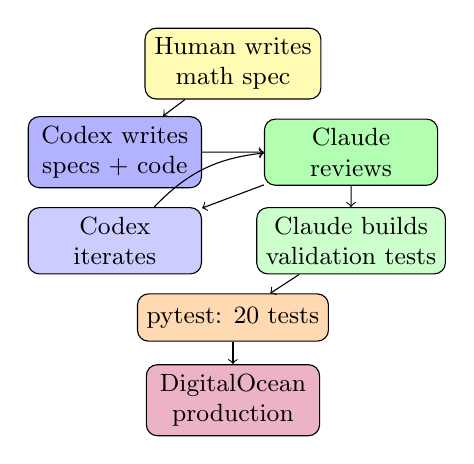
\begin{tikzpicture}[scale=0.75,
    box/.style={rectangle, draw, rounded corners, minimum width=2.2cm, minimum height=0.6cm, align=center, font=\small}]

    \node[box, fill=yellow!30] (human) at (0,4) {Human writes\\math spec};
    \node[box, fill=blue!30] (codex1) at (-2,2.5) {Codex writes\\specs + code};
    \node[box, fill=green!30] (claude1) at (2,2.5) {Claude\\reviews};
    \node[box, fill=blue!20] (codex2) at (-2,1) {Codex\\iterates};
    \node[box, fill=green!20] (claude2) at (2,1) {Claude builds\\validation tests};
    \node[box, fill=orange!30] (pytest) at (0,-0.3) {pytest: 20 tests};
    \node[box, fill=purple!30] (deploy) at (0,-1.7) {DigitalOcean\\production};

    \draw[->] (human) -- (codex1);
    \draw[->] (codex1) -- (claude1);
    \draw[->] (claude1) -- (codex2);
    \draw[->] (claude1) -- (claude2);
    \draw[->] (codex2) to[bend left=20] (claude1);
    \draw[->] (claude2) -- (pytest);
    \draw[->] (pytest) -- (deploy);
\end{tikzpicture}
\end{center}

\textbf{Iteration:} Multiple cycles until all 20 tests pass
\end{frame}

\begin{frame}{Zero-Intervention Automation Pipeline}
\textbf{A Hobby Project with Production-Grade Rigor:}

One prompt triggers the \textbf{entire pipeline} --- no human intervention:

\begin{enumerate}
    \item \textcolor{blue!70}{\textbf{Coding}} --- AI implements from specs
    \item \textcolor{orange!70}{\textbf{Regression Testing}} --- pytest runs 20+ tests locally
    \item \textcolor{purple!70}{\textbf{Browser UI Testing}} --- Playwright validates Flask UI
    \item \textcolor{green!70}{\textbf{Documentation}} --- LaTeX auto-updated
    \item \textcolor{cyan!70}{\textbf{Deploy to DigitalOcean}} --- SSH + Git + systemd
    \item \textcolor{orange!70}{\textbf{Production Regression}} --- Tests on live server
    \item \textcolor{red!70}{\textbf{Telegram Notification}} --- ``Done!''
\end{enumerate}

\vspace{0.2cm}
\begin{center}
\fbox{\parbox{0.85\textwidth}{
\textbf{Key Insight:} \$7/month hobby project built with the same rigor as top tech company production systems.
}}
\end{center}
\end{frame}

\begin{frame}{QuantLib Extension Strategy}
\textbf{QuantLib's Limitations:}
\begin{itemize}
    \item No native callable XCCY support
    \item Limited multi-currency Monte Carlo
    \item No built-in LSM for cross-currency
\end{itemize}

\textbf{How We Extended It (Collaboratively):}
\begin{enumerate}
    \item \textbf{Human:} Defined what QuantLib provides vs what's needed
    \item \textbf{Codex:} Wrote custom Monte Carlo using QuantLib curves
    \item \textbf{Claude:} Verified QuantLib API usage against docs
    \item \textbf{Stack Overflow:} Confirmed edge cases and patterns
\end{enumerate}

\textbf{Result:}
\begin{itemize}
    \item Use QuantLib for: curves, dates, calendars, basic calibration
    \item Custom code for: multi-factor MC, LSM, XCCY cashflows
    \item 1,400+ lines of rigorous extensions
\end{itemize}
\end{frame}

\begin{frame}[fragile]{DigitalOcean Deployment: Detailed Steps}
\textbf{1. Droplet Creation (DigitalOcean Console):}
\begin{itemize}
    \item Region: NYC3 or SFO3 for US users
    \item Image: Ubuntu 22.04 LTS
    \item Plan: Basic \$7/month (2GB RAM, 1 vCPU) --- hobby-friendly!
    \item Authentication: SSH key (not password)
\end{itemize}

\textbf{2. Initial Server Setup:}
\begin{verbatim}
ssh root@your-droplet-ip
apt update && apt upgrade -y
adduser deploy
usermod -aG sudo deploy
\end{verbatim}

\textbf{3. Application Deployment:}
\begin{verbatim}
cd /opt && git clone <repo>
python3 -m venv .venv
.venv/bin/pip install -r requirements.txt
cp deploy/systemd/*.template /etc/systemd/system/
systemctl enable --now tgir-quantlib-tools
\end{verbatim}
\end{frame}

\begin{frame}[fragile]{DigitalOcean: SSL and Apache Configuration}
\textbf{Apache Setup:}
\begin{verbatim}
apt install apache2
a2enmod proxy proxy_http ssl rewrite
cp deploy/apache/*.template /etc/apache2/sites-available/
a2ensite tgir-quantlib-tools
systemctl reload apache2
\end{verbatim}

\textbf{SSL with Certbot:}
\begin{verbatim}
apt install certbot python3-certbot-apache
certbot --apache -d your-domain.com
\end{verbatim}

\textbf{Firewall:}
\begin{verbatim}
ufw allow 22/tcp
ufw allow 80/tcp
ufw allow 443/tcp
ufw enable
\end{verbatim}

\textbf{Result:} HTTPS-secured Flask app at \texttt{https://your-domain.com}
\end{frame}

\begin{frame}{Why Codex + Claude Collaboration Works}
\textbf{Complementary Strengths:}
\begin{itemize}
    \item \textbf{Codex:} Excellent at ground-up implementation from specs
    \item \textbf{Claude:} Excellent at review, validation, extension
    \item \textbf{Human:} Domain expertise, orchestration, final judgment
\end{itemize}

\textbf{Error Detection:}
\begin{itemize}
    \item Claude catches bugs in Codex's implementations
    \item Codex fixes issues Claude identifies
    \item Neither alone would produce same quality
\end{itemize}

\textbf{Stack Overflow Role:}
\begin{itemize}
    \item AI can hallucinate APIs that don't exist
    \item Human experts catch edge cases
    \item Community validates approaches
\end{itemize}

\textbf{Key Lesson:}\\[0.2cm]
\fbox{\parbox{0.85\textwidth}{\centering Two AI agents + human domain expert\\produces better results than any single agent}}
\end{frame}

\begin{frame}{The Methodology IS the Innovation}
\textbf{This project delivers TWO things:}

\begin{enumerate}
    \item \textbf{Callable XCCY Pricer:}
    \begin{itemize}
        \item Three-factor Monte Carlo
        \item Longstaff-Schwartz optimization
        \item 20 validation tests
        \item Production deployment
    \end{itemize}

    \item \textbf{Collaborative Development Methodology:}
    \begin{itemize}
        \item Human $\to$ Codex (specs, implementation)
        \item Codex $\to$ Claude (review, validation)
        \item Claude $\to$ Regression tests (future-proofing)
        \item Full ecosystem: Mac + DigitalOcean + QuantLib + Python
    \end{itemize}
\end{enumerate}

\vspace{0.3cm}
\textbf{The methodology is reusable for other complex pricers}

\fbox{\parbox{0.85\textwidth}{\centering The collaborative workflow is as valuable as the callable XCCY pricer itself}}
\end{frame}

\begin{frame}{Reusable Human-Agent Development Pattern}
\begin{center}
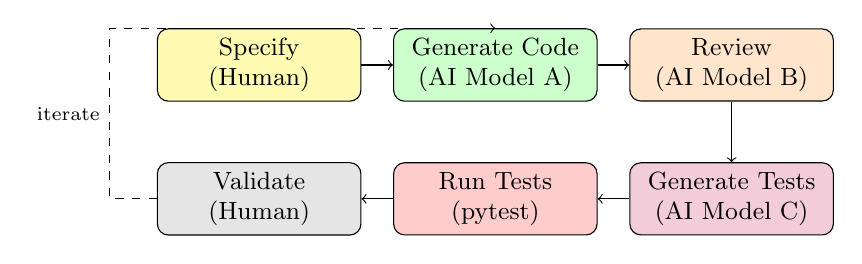
\begin{tikzpicture}[
    box/.style={rectangle, draw, rounded corners, text width=2.35cm, minimum height=0.9cm, align=center, font=\small}]
    \node[box, fill=yellow!30] (spec) at (-3,2.4) {Specify\\(Human)};
    \node[box, fill=green!20] (gen) at (0,2.4) {Generate Code\\(AI Model A)};
    \node[box, fill=orange!20] (review) at (3,2.4) {Review\\(AI Model B)};
    \node[box, fill=purple!20] (test) at (3,0.7) {Generate Tests\\(AI Model C)};
    \node[box, fill=red!20] (run) at (0,0.7) {Run Tests\\(pytest)};
    \node[box, fill=gray!20] (valid) at (-3,0.7) {Validate\\(Human)};

    \draw[->] (spec) -- (gen);
    \draw[->] (gen) -- (review);
    \draw[->] (review) -- (test);
    \draw[->] (test) -- (run);
    \draw[->] (run) -- (valid);
    \draw[->, dashed] (valid.west) -- ++(-0.6,0) |- node[pos=0.25,left,font=\scriptsize] {iterate} (gen.north);
\end{tikzpicture}
\end{center}

\textbf{Key Principle:}\\[0.3cm]
\fbox{\parbox{0.85\textwidth}{\centering Human provides specifications and validation\\AI accelerates implementation and review}}
\end{frame}

\begin{frame}{}
\begin{center}
\Huge\textbf{End of Supplementary Material}\\[2cm]
\Large Return to Main Presentation
\end{center}
\end{frame}

\end{document}

% Or compile separately

\documentclass[aspectratio=169,11pt]{beamer}
\usepackage[T1]{fontenc}
\usepackage[utf8]{inputenc}
\usepackage{lmodern}
\usepackage{mastering_ir_derivatives_beamer_1.0}
\usepackage{booktabs}
\usepackage{array}
\usepackage{listings}

% Retain the supplied visual system without changing the authored slide count.
\beamerdefaultoverlayspecification{<*>}
\AtBeginSection[]{}
\AtBeginSubsection[]{}

\hypersetup{
    colorlinks=true,
    linkcolor=blue,
    urlcolor=blue
}

\lstset{
    basicstyle=\ttfamily\scriptsize,
    breaklines=true,
    columns=fullflexible
}

\newcommand{\product}{TGIR QuantLib Tools}
\newcommand{\code}[1]{\texttt{#1}}
\newcommand{\docdate}{2026-04-06}


\usepackage[utf8]{inputenc}
\usepackage{amsmath,amssymb}
\usepackage{booktabs}
\usepackage{multirow}
\usepackage{listings}
\usepackage{tikz}
\usepackage{xcolor}

\lstset{
    language=Python,
    basicstyle=\ttfamily\scriptsize,
    keywordstyle=\color{blue}\bfseries,
    commentstyle=\color{green!50!black},
    stringstyle=\color{red},
    showstringspaces=false,
    breaklines=true,
    frame=single,
    backgroundcolor=\color{gray!10}
}

\title[Supplementary Content]{\textbf{QuantLib Derivatives Pricing}\\Supplementary Technical Slides}
\author{Quantitative Analytics Team}
\date{August 2026}

\begin{document}

%%%%%%%%%%%%%%%%%%%%%%%%%%%%%%%%%%%%%%%%%%%%%%%%%%%%%%%%%%%%%%%%%%%%%%%%%%%%%%%%
%% APPENDIX A: MATHEMATICAL FOUNDATIONS (20 slides)
%%%%%%%%%%%%%%%%%%%%%%%%%%%%%%%%%%%%%%%%%%%%%%%%%%%%%%%%%%%%%%%%%%%%%%%%%%%%%%%%

\begin{frame}
\titlepage
\end{frame}

\begin{frame}{}
\begin{center}
\Huge\textbf{Appendix A}\\[1cm]
\Large Mathematical Foundations\\[0.5cm]
\normalsize Stochastic Calculus Essentials
\end{center}
\end{frame}

\begin{frame}{Brownian Motion: Definition}
\begin{block}{Standard Brownian Motion $W_t$}
A stochastic process with:
\begin{enumerate}
    \item $W_0 = 0$
    \item Independent increments: $W_t - W_s \perp W_s - W_u$ for $t > s > u$
    \item Normally distributed: $W_t - W_s \sim N(0, t-s)$
    \item Continuous paths
\end{enumerate}
\end{block}

\textbf{Key Properties:}
\begin{itemize}
    \item $\mathbb{E}[W_t] = 0$
    \item $\text{Var}[W_t] = t$
    \item $\mathbb{E}[W_t W_s] = \min(t, s)$
    \item Paths are nowhere differentiable
\end{itemize}
\end{frame}

\begin{frame}{Itô's Lemma}
\begin{block}{Itô's Formula}
For $f(t, X_t)$ where $dX_t = \mu\,dt + \sigma\,dW_t$:
\[
df = \frac{\partial f}{\partial t}dt + \frac{\partial f}{\partial x}dX_t + \frac{1}{2}\frac{\partial^2 f}{\partial x^2}\sigma^2 dt
\]
\end{block}

\textbf{Example: Geometric Brownian Motion}

Let $S_t$ follow $dS_t = \mu S_t\,dt + \sigma S_t\,dW_t$. Apply Itô to $f(S) = \ln S$:
\[
d\ln S = \frac{1}{S}dS - \frac{1}{2}\frac{1}{S^2}\sigma^2 S^2 dt = \left(\mu - \frac{\sigma^2}{2}\right)dt + \sigma\,dW_t
\]

Therefore: $S_T = S_0 \exp\left[(\mu - \frac{\sigma^2}{2})T + \sigma W_T\right]$
\end{frame}

\begin{frame}{Risk-Neutral Pricing}
\begin{block}{Fundamental Theorem of Asset Pricing}
No-arbitrage $\Leftrightarrow$ Exists a probability measure $\mathbb{Q}$ such that discounted asset prices are martingales.
\end{block}

\textbf{Pricing Formula:}
\[
V_0 = \mathbb{E}^\mathbb{Q}\left[e^{-\int_0^T r_s\,ds} \cdot \text{Payoff}_T\right]
\]

\textbf{Change of Measure (Girsanov):}
\begin{itemize}
    \item Under $\mathbb{P}$: $dS = \mu S\,dt + \sigma S\,dW^\mathbb{P}$
    \item Under $\mathbb{Q}$: $dS = r S\,dt + \sigma S\,dW^\mathbb{Q}$
    \item $dW^\mathbb{Q} = dW^\mathbb{P} + \frac{\mu - r}{\sigma}dt$
\end{itemize}
\end{frame}

\begin{frame}{Ornstein-Uhlenbeck Process}
\begin{block}{OU Process}
\[
dx_t = -a x_t\,dt + \sigma\,dW_t
\]
\end{block}

\textbf{Solution:}
\[
x_t = x_0 e^{-at} + \sigma \int_0^t e^{-a(t-s)}\,dW_s
\]

\textbf{Properties:}
\begin{itemize}
    \item Mean: $\mathbb{E}[x_t] = x_0 e^{-at}$
    \item Variance: $\text{Var}[x_t] = \frac{\sigma^2}{2a}(1 - e^{-2at})$
    \item Stationary distribution: $N(0, \frac{\sigma^2}{2a})$
    \item Auto-correlation: $\text{Corr}(x_t, x_s) = e^{-a|t-s|}$
\end{itemize}

\textbf{Hull-White:} Add time-dependent mean $\theta(t)$
\end{frame}

\begin{frame}{Affine Term Structure Models}
\begin{block}{Affine Property}
Discount bond prices have the form:
\[
P(t, T) = e^{A(t,T) - B(t,T) r_t}
\]
\end{block}

\textbf{For Hull-White:}
\[
B(t, T) = \frac{1 - e^{-a(T-t)}}{a}
\]
\[
A(t, T) = \int_t^T \theta(s) B(s, T)\,ds - \frac{\sigma^2}{2}\int_t^T B(s, T)^2\,ds
\]

\textbf{Implications:}
\begin{itemize}
    \item Analytical bond and swaption prices
    \item Efficient calibration
    \item Foundation for tree methods
\end{itemize}
\end{frame}

\begin{frame}{Multi-Factor Models: Correlated Brownians}
\textbf{Correlated Brownian Motions:}

Given correlation matrix $\mathbf{R}$, generate correlated increments:
\[
\begin{pmatrix} dW_1 \\ dW_2 \\ dW_3 \end{pmatrix} = \mathbf{L} \cdot \begin{pmatrix} dZ_1 \\ dZ_2 \\ dZ_3 \end{pmatrix}
\]

Where $\mathbf{L}$ is the Cholesky decomposition: $\mathbf{R} = \mathbf{L}\mathbf{L}^T$

\textbf{Example:} $\rho_{12} = 0.25$, $\rho_{13} = -0.15$, $\rho_{23} = -0.30$

\[
\mathbf{L} = \begin{pmatrix}
1 & 0 & 0 \\
0.25 & 0.968 & 0 \\
-0.15 & -0.271 & 0.951
\end{pmatrix}
\]
\end{frame}

\begin{frame}{Variance Calculation for Joint Processes}
\textbf{For state $\mathbf{x}_t$:}
\[
\text{Cov}[\mathbf{x}_{t+h}, \mathbf{x}_{t+h}] = \int_0^h \mathbf{K}(s) \cdot \mathbf{R} \cdot \mathbf{K}(s)^T\,ds
\]

Where $\mathbf{K}(s)$ is the kernel matrix mapping Brownians to state.

\textbf{Numerical Integration:}
\[
\int_0^h f(s)\,ds \approx \frac{h}{2}\sum_{i=1}^{n} w_i f\left(\frac{h}{2}(x_i + 1)\right)
\]

Using Gauss-Legendre nodes $x_i$ and weights $w_i$.

\textbf{Our Implementation:} 16-point Gauss-Legendre quadrature
\end{frame}

\begin{frame}{Change of Numéraire}
\begin{block}{Numéraire Change}
When changing from numéraire $N_1$ to $N_2$:
\[
\frac{d\mathbb{Q}^{N_2}}{d\mathbb{Q}^{N_1}}\bigg|_{\mathcal{F}_T} = \frac{N_2(T) / N_2(0)}{N_1(T) / N_1(0)}
\]
\end{block}

\textbf{FX Pricing Application:}

Under USD money-market measure:
\begin{itemize}
    \item USD bank account is numéraire
    \item EUR rates get quanto adjustment
    \item FX drift includes rate differential
\end{itemize}

\[
d\ln X = (r^{USD} - r^{EUR} - \tfrac{1}{2}\sigma_X^2)\,dt + \sigma_X\,dW_X
\]
\end{frame}

\begin{frame}{Quanto Adjustment Derivation}
\textbf{Setting:} Price a EUR asset $S^{EUR}$ from USD perspective

\textbf{Under EUR measure:}
\[
dS^{EUR} = r^{EUR} S^{EUR}\,dt + \sigma_S S^{EUR}\,dW_S^{EUR}
\]

\textbf{Converting to USD measure:}
\[
dS^{EUR} = (r^{EUR} - \rho_{S,X}\sigma_S\sigma_X) S^{EUR}\,dt + \sigma_S S^{EUR}\,dW_S^{USD}
\]

\textbf{Intuition:}
\begin{itemize}
    \item If $\rho_{S,X} > 0$: Asset rises when EUR appreciates
    \item Extra expected USD return from FX
    \item Must subtract to stay risk-neutral
\end{itemize}
\end{frame}

%%%%%%%%%%%%%%%%%%%%%%%%%%%%%%%%%%%%%%%%%%%%%%%%%%%%%%%%%%%%%%%%%%%%%%%%%%%%%%%%
%% APPENDIX B: QUANTLIB DEEP DIVE (20 slides)
%%%%%%%%%%%%%%%%%%%%%%%%%%%%%%%%%%%%%%%%%%%%%%%%%%%%%%%%%%%%%%%%%%%%%%%%%%%%%%%%

\begin{frame}{}
\begin{center}
\Huge\textbf{Appendix B}\\[1cm]
\Large QuantLib Deep Dive\\[0.5cm]
\normalsize Internal Architecture and APIs
\end{center}
\end{frame}

\begin{frame}{QuantLib Class Hierarchy}
\begin{center}
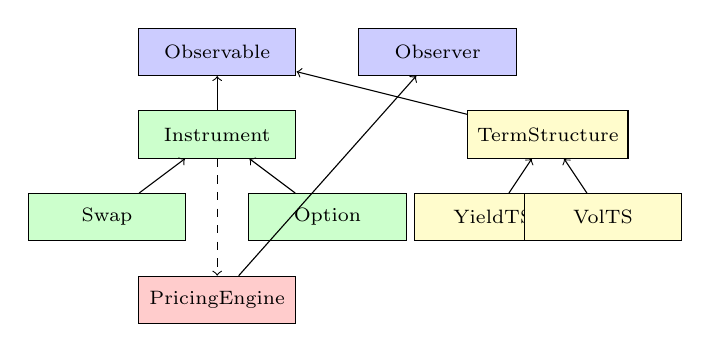
\begin{tikzpicture}[scale=0.7,
    box/.style={rectangle, draw, minimum width=2cm, minimum height=0.6cm, font=\scriptsize}]

    % Observer pattern
    \node[box, fill=blue!20] (obs) at (0,4) {Observable};
    \node[box, fill=blue!20] (obsr) at (4,4) {Observer};

    % Instruments
    \node[box, fill=green!20] (inst) at (0,2.5) {Instrument};
    \node[box, fill=green!20] (swap) at (-2,1) {Swap};
    \node[box, fill=green!20] (opt) at (2,1) {Option};

    % Term structures
    \node[box, fill=yellow!20] (ts) at (6,2.5) {TermStructure};
    \node[box, fill=yellow!20] (yts) at (5,1) {YieldTS};
    \node[box, fill=yellow!20] (vts) at (7,1) {VolTS};

    % Engines
    \node[box, fill=red!20] (eng) at (0,-0.5) {PricingEngine};

    \draw[->] (inst) -- (obs);
    \draw[->] (swap) -- (inst);
    \draw[->] (opt) -- (inst);
    \draw[->] (ts) -- (obs);
    \draw[->] (yts) -- (ts);
    \draw[->] (vts) -- (ts);
    \draw[->] (eng) -- (obsr);
    \draw[dashed,->] (inst) -- (eng);
\end{tikzpicture}
\end{center}

\textbf{Key Patterns:}
\begin{itemize}
    \item Observer/Observable for lazy evaluation
    \item Instruments are priced by Engines
    \item Term structures hold market data
\end{itemize}
\end{frame}

\begin{frame}[fragile]{Date and Calendar Handling}
\begin{lstlisting}[language=Python]
import QuantLib as ql

# Date construction
d1 = ql.Date(15, 8, 2026)           # Day, Month, Year
d2 = ql.Date(15, ql.August, 2026)   # Using enum
d3 = ql.DateParser.parseISO("2026-08-15")

# Date arithmetic
d4 = d1 + ql.Period(3, ql.Months)
d5 = d1 + 30  # Add 30 calendar days

# Calendar operations
cal = ql.UnitedStates(ql.UnitedStates.Settlement)
if cal.isBusinessDay(d1):
    print("Business day")

# Advance by business days
spot = cal.advance(d1, 2, ql.Days)

# Joint calendar (requires both to be open)
joint = ql.JointCalendar(ql.TARGET(),
    ql.UnitedStates(ql.UnitedStates.Settlement),
    ql.JoinHolidays)
\end{lstlisting}
\end{frame}

\begin{frame}[fragile]{Index Classes}
\begin{lstlisting}[language=Python]
# Overnight indices
sofr = ql.Sofr()
estr = ql.Estr()
sonia = ql.Sonia()

# Link to curve
curve_handle = ql.YieldTermStructureHandle(curve)
sofr_with_curve = ql.Sofr(curve_handle)

# Get fixings
fixing_date = ql.Date(10, 8, 2026)
rate = sofr.fixing(fixing_date)

# Add historical fixings (for backward-looking)
ql.IndexManager.instance().clearHistories()
sofr.addFixing(ql.Date(1, 8, 2026), 0.04)
sofr.addFixing(ql.Date(2, 8, 2026), 0.0402)
\end{lstlisting}
\end{frame}

\begin{frame}[fragile]{Yield Curve Construction Details}
\begin{lstlisting}[language=Python]
# Rate helpers
helpers = []

# Deposit helper (for short end)
helpers.append(ql.DepositRateHelper(
    ql.QuoteHandle(ql.SimpleQuote(0.041)),  # Rate
    ql.Period(1, ql.Days),                   # Tenor
    0,                                        # Settlement days
    ql.UnitedStates(ql.UnitedStates.Settlement),
    ql.ModifiedFollowing,                    # Convention
    False,                                   # End of month
    ql.Actual360()                          # Day count
))

# OIS helpers
for tenor, rate in [("1Y", 0.039), ("5Y", 0.037)]:
    helpers.append(ql.OISRateHelper(
        2, ql.Period(tenor),
        ql.QuoteHandle(ql.SimpleQuote(rate)),
        ql.Sofr()
    ))

# Build curve
curve = ql.PiecewiseLogLinearDiscount(today, helpers, ql.Actual365Fixed())
curve.enableExtrapolation()
\end{lstlisting}
\end{frame}

\begin{frame}[fragile]{OvernightIndexedSwap Instrument}
\begin{lstlisting}[language=Python]
# Create OIS swap
schedule = ql.Schedule(
    start_date, end_date,
    ql.Period(ql.Semiannual),          # Payment frequency
    calendar,
    ql.ModifiedFollowing,              # Business day convention
    ql.ModifiedFollowing,
    ql.DateGeneration.Backward,
    False                              # End of month
)

swap = ql.OvernightIndexedSwap(
    ql.Swap.Payer,                     # Type
    100_000_000.0,                     # Notional
    schedule,
    0.04,                              # Fixed rate
    ql.Actual360(),                    # Fixed day count
    ql.Sofr(curve_handle),             # Index
    0.0,                               # Spread on floating
    0,                                 # Payment lag
    ql.ModifiedFollowing,
    calendar
)
\end{lstlisting}
\end{frame}

\begin{frame}[fragile]{Swaption Construction}
\begin{lstlisting}[language=Python]
# Create underlying swap
underlying = ql.VanillaSwap(
    ql.Swap.Payer, notional,
    fixed_schedule, strike, day_count,
    float_schedule, sofr_index, 0.0, day_count
)

# European exercise
expiry = ql.Date(15, 8, 2028)
exercise = ql.EuropeanExercise(expiry)

# Bermudan exercise
call_dates = [ql.Date(15, 8, 2028 + i) for i in range(5)]
exercise = ql.BermudanExercise(call_dates)

# Create swaption
swaption = ql.Swaption(underlying, exercise)

# Set pricing engine
engine = ql.TreeSwaptionEngine(hw_model, 50)
swaption.setPricingEngine(engine)

print(f"NPV: {swaption.NPV():,.2f}")
\end{lstlisting}
\end{frame}

\begin{frame}[fragile]{Hull-White Model Setup}
\begin{lstlisting}[language=Python]
# Create model with fixed parameters
mean_reversion = 0.03
volatility = 0.01
model = ql.HullWhite(curve_handle, mean_reversion, volatility)

# Get model parameters
params = model.params()
print(f"a = {params[0]}, sigma = {params[1]}")

# Create calibration helpers
helpers = []
for expiry, tenor, vol_bp in [("2Y", "8Y", 78), ("5Y", "5Y", 80)]:
    helper = ql.SwaptionHelper(
        ql.Period(expiry), ql.Period(tenor),
        ql.QuoteHandle(ql.SimpleQuote(vol_bp * 1e-4)),
        sofr_index, ql.Period("1Y"), ql.Actual360(),
        ql.Actual360(), curve_handle,
        ql.BlackCalibrationHelper.RelativePriceError,
        ql.nullDouble(), 1.0, ql.Normal
    )
    helper.setPricingEngine(ql.JamshidianSwaptionEngine(model))
    helpers.append(helper)
\end{lstlisting}
\end{frame}

\begin{frame}[fragile]{Model Calibration}
\begin{lstlisting}[language=Python]
# Calibration settings
opt_method = ql.LevenbergMarquardt()
end_criteria = ql.EndCriteria(
    500,    # Max iterations
    100,    # Max stationary
    1e-10,  # Root epsilon
    1e-10,  # Function epsilon
    1e-10   # Gradient epsilon
)

# Which parameters to calibrate
# [True, False] means calibrate a, keep sigma fixed
fixed_params = ql.BoolVector([True, False])

# Run calibration
model.calibrate(
    helpers,        # Calibration instruments
    opt_method,
    end_criteria,
    ql.PositiveConstraint(),  # Parameter constraint
    ql.DoubleVector(),        # Weights
    fixed_params
)

# Check results
print(f"Calibrated sigma: {model.params()[1]:.6f}")
\end{lstlisting}
\end{frame}

\begin{frame}[fragile]{Calibration Diagnostics}
\begin{lstlisting}[language=Python]
# After calibration, check fit quality
for i, helper in enumerate(helpers):
    market_val = helper.marketValue()
    model_val = helper.modelValue()
    error = (model_val - market_val) / market_val

    # Get implied vol
    impl_vol = helper.impliedVolatility(model_val, 1e-6, 100,
                                         1e-6, 2.0)

    print(f"Helper {i}:")
    print(f"  Market: {market_val:.6f}")
    print(f"  Model:  {model_val:.6f}")
    print(f"  Error:  {error*100:.3f}%")
    print(f"  Impl Vol: {impl_vol*10000:.1f}bp")

# Calculate weighted RMS
errors = [(h.modelValue()/h.marketValue() - 1)**2 for h in helpers]
rms = math.sqrt(sum(errors) / len(errors))
print(f"RMS Error: {rms*100:.3f}%")
\end{lstlisting}
\end{frame}

\begin{frame}{QuantLib Limitations for XCCY}
\textbf{Native XCCY Support:}
\begin{itemize}
    \item \texttt{CrossCurrencyBasisSwap} --- exists for vanilla XCCY
    \item \texttt{CrossCurrencyBasisSwapRateHelper} --- for curve building
    \item No native \textbf{callable} XCCY instrument
\end{itemize}

\textbf{Multi-Factor Limitations:}
\begin{itemize}
    \item Tree engines work for 1-2 factors
    \item No native 3-factor joint tree
    \item Would need FD solver on 3D grid (slow)
    \item Monte Carlo is natural choice
\end{itemize}

\textbf{Our Solution:}
\begin{itemize}
    \item Use QuantLib for curves, dates, indices
    \item Custom 3-factor Monte Carlo
    \item LSM for exercise optimization
\end{itemize}
\end{frame}

%%%%%%%%%%%%%%%%%%%%%%%%%%%%%%%%%%%%%%%%%%%%%%%%%%%%%%%%%%%%%%%%%%%%%%%%%%%%%%%%
%% APPENDIX C: MONTE CARLO METHODS (20 slides)
%%%%%%%%%%%%%%%%%%%%%%%%%%%%%%%%%%%%%%%%%%%%%%%%%%%%%%%%%%%%%%%%%%%%%%%%%%%%%%%%

\begin{frame}{}
\begin{center}
\Huge\textbf{Appendix C}\\[1cm]
\Large Monte Carlo Methods\\[0.5cm]
\normalsize Simulation Techniques and Variance Reduction
\end{center}
\end{frame}

\begin{frame}{Monte Carlo Basics}
\begin{block}{Law of Large Numbers}
\[
\frac{1}{N}\sum_{i=1}^{N} f(X_i) \xrightarrow{N\to\infty} \mathbb{E}[f(X)]
\]
\end{block}

\textbf{Standard Error:}
\[
SE = \frac{\sigma}{\sqrt{N}}
\]

\textbf{95\% Confidence Interval:}
\[
\bar{X} \pm 1.96 \times SE
\]

\textbf{Key Properties:}
\begin{itemize}
    \item Error decreases as $O(N^{-1/2})$
    \item Independent of dimension (curse of dimensionality avoided)
    \item Flexible for path-dependent payoffs
\end{itemize}
\end{frame}

\begin{frame}[fragile]{Random Number Generation}
\textbf{NumPy PCG64 Generator:}
\begin{itemize}
    \item Permuted Congruential Generator
    \item Period: $2^{128}$
    \item Excellent statistical properties
    \item Fast and reproducible
\end{itemize}

\textbf{Usage:}
\begin{lstlisting}[language=Python]
import numpy as np

# Create generator with seed
rng = np.random.Generator(np.random.PCG64(1729))

# Generate standard normals
Z = rng.standard_normal((paths, dimensions))
\end{lstlisting}

\textbf{Reproducibility:}
\begin{itemize}
    \item Same seed $\Rightarrow$ same sequence
    \item Critical for debugging and validation
\end{itemize}
\end{frame}

\begin{frame}[fragile]{Variance Reduction: Antithetic Variates}
\begin{block}{Antithetic Sampling}
If $\hat{\theta}_1 = f(Z)$ and $\hat{\theta}_2 = f(-Z)$ are negatively correlated, then:
\[
\text{Var}\left[\frac{\hat{\theta}_1 + \hat{\theta}_2}{2}\right] < \text{Var}[\hat{\theta}_1]
\]
\end{block}

\textbf{Implementation:}
\begin{lstlisting}[language=Python]
def antithetic_normals(rng, paths, dims):
    half = (paths + 1) // 2
    draws = rng.standard_normal((half, dims))
    return np.concatenate([draws, -draws])[:paths]
\end{lstlisting}

\textbf{Benefits:}
\begin{itemize}
    \item Forces mean of normals to be exactly 0
    \item Reduces variance for most payoffs
    \item No additional cost per sample
\end{itemize}
\end{frame}

\begin{frame}{Variance Reduction: Control Variates}
\begin{block}{Control Variate Method}
Use a correlated variable $Y$ with known mean $\mu_Y$:
\[
\hat{\theta}_{CV} = \hat{\theta} - \beta(\bar{Y} - \mu_Y)
\]
\end{block}

\textbf{Optimal $\beta$:}
\[
\beta^* = \frac{\text{Cov}[\hat{\theta}, Y]}{\text{Var}[Y]}
\]

\textbf{Applications in Derivatives:}
\begin{itemize}
    \item Use underlying asset as control
    \item Use European price for Bermudan
    \item Use delta-hedged portfolio
\end{itemize}
\end{frame}

\begin{frame}{Quasi-Monte Carlo (QMC)}
\textbf{Low-Discrepancy Sequences:}
\begin{itemize}
    \item Sobol, Halton, Niederreiter
    \item Fill space more uniformly than random
    \item Error $O(N^{-1})$ vs $O(N^{-1/2})$
\end{itemize}

\textbf{Trade-offs:}
\begin{itemize}
    \item Better for smooth integrands
    \item Dimension-dependent effectiveness
    \item Standard error not directly computable
\end{itemize}

\textbf{Not used in our implementation:}
\begin{itemize}
    \item Standard MC simpler to implement
    \item Antithetic sufficient for our accuracy needs
    \item QMC would be future enhancement
\end{itemize}
\end{frame}

\begin{frame}{Path Generation: Euler vs Exact}
\textbf{Euler Discretization:}
\[
x_{t+\Delta t} = x_t + \mu(x_t)\Delta t + \sigma(x_t)\sqrt{\Delta t}\, Z
\]

\textbf{Exact Simulation (OU process):}
\[
x_{t+h} = x_t e^{-ah} + \sigma\int_0^h e^{-a(h-s)}\,dW_s
\]

\textbf{Our Approach: Exact OU Kernels}
\begin{itemize}
    \item Hull-White factors use exact solution
    \item No discretization bias
    \item Larger time steps possible
    \item Covariance computed exactly
\end{itemize}
\end{frame}

\begin{frame}[fragile]{State Evolution Implementation}
\begin{lstlisting}[language=Python]
@dataclass
class StepTransition:
    matrix: np.ndarray      # Transition matrix A
    offset: np.ndarray      # Deterministic drift b
    covariance_root: np.ndarray  # sqrt(Sigma)

def evolve_state(state, transition, normals):
    """
    x_{t+h} = A * x_t + b + L * Z

    state: (paths, 5) current state
    transition: StepTransition object
    normals: (paths, 5) standard normals

    Returns: (paths, 5) new state
    """
    return (state @ transition.matrix.T
            + transition.offset
            + normals @ transition.covariance_root.T)
\end{lstlisting}
\end{frame}

\begin{frame}{Cash Flow Valuation}
\textbf{For each simulated path:}

\textbf{Fixed Cash Flow:}
\[
PV = \text{Amount} \times e^{-I_{USD}(t_{pay})}
\]

\textbf{Floating Cash Flow (compounded overnight):}
\[
\text{Amount} = N \times \left(e^{I_{EUR}(t_{end}) - I_{EUR}(t_{start}) + \text{basis}} - 1\right)
\]
\[
PV = \text{Amount} \times X_{t_{pay}} \times e^{-I_{USD}(t_{pay})}
\]

\textbf{FX Conversion:} EUR amounts converted at simulated FX rate

\textbf{Notional Exchanges:}
\begin{itemize}
    \item Initial: Net of notionals at spot
    \item Final: Net of notionals at terminal FX
\end{itemize}
\end{frame}

\begin{frame}{LSM: Basis Function Selection}
\textbf{State Variables:} $(x_{USD}, x_{EUR}, \ln X - \ln X_0)$

\textbf{Polynomial Basis (10 functions):}
\[
\phi = (1,\, x,\, y,\, z,\, x^2,\, y^2,\, z^2,\, xy,\, xz,\, yz)
\]

\textbf{Why This Choice?}
\begin{itemize}
    \item Captures main effects (linear terms)
    \item Captures curvature (squared terms)
    \item Captures interactions (cross terms)
    \item Low-dimensional (avoids overfitting)
\end{itemize}

\textbf{Alternatives:}
\begin{itemize}
    \item Laguerre polynomials
    \item Chebyshev polynomials
    \item Neural network approximation
\end{itemize}
\end{frame}

\begin{frame}{LSM: Numerical Stability}
\textbf{Problem: Ill-Conditioned Design Matrix}

When state variables have different scales or are correlated:
\[
\text{cond}(\mathbf{X}^T\mathbf{X}) \gg 1
\]

\textbf{Solutions:}
\begin{enumerate}
    \item \textbf{Standardization:}
    \[
    \tilde{x} = \frac{x - \bar{x}}{\sigma_x}
    \]

    \item \textbf{Ridge Regression:}
    \[
    \boldsymbol{\beta} = (\mathbf{X}^T\mathbf{X} + \lambda\mathbf{I})^{-1}\mathbf{X}^T\mathbf{y}
    \]
\end{enumerate}

\textbf{Our Implementation:}
\begin{itemize}
    \item Standardize state variables
    \item Use \texttt{np.linalg.lstsq} with rcond
    \item Fall back to ridge if cond $>$ 1e10
\end{itemize}
\end{frame}

\begin{frame}{LSM: Two-Pass Why It Matters}
\textbf{Single-Pass Bias:}
\begin{itemize}
    \item Training on same paths as pricing
    \item Exercise decision uses future information
    \item Results in upward bias (too high)
\end{itemize}

\textbf{Two-Pass Solution:}
\begin{enumerate}
    \item \textbf{Training Pass:} Learn policy on paths 1...N
    \item \textbf{Pricing Pass:} Apply policy on paths N+1...2N
\end{enumerate}

\textbf{Properties:}
\begin{itemize}
    \item Pricing paths are independent of training
    \item No look-ahead bias
    \item Result is a \textit{lower bound} on true value
\end{itemize}

\textbf{Why Lower Bound?}
\begin{itemize}
    \item Suboptimal exercise policy
    \item True optimal policy would give higher value
    \item Upper bound requires dual methods
\end{itemize}
\end{frame}

\begin{frame}{Convergence Diagnostics}
\textbf{Standard Error Analysis:}
\[
SE = \frac{\sigma}{\sqrt{N}}
\]

\textbf{Expected Behavior:}
\begin{itemize}
    \item Double paths $\Rightarrow$ SE reduces by $\sqrt{2}$
    \item 10x paths $\Rightarrow$ SE reduces by $\sqrt{10} \approx 3.16$
\end{itemize}

\textbf{Test Protocol:}
\begin{enumerate}
    \item Run with 10K paths, record SE
    \item Run with 40K paths, record SE
    \item Verify ratio $\approx$ 2.0
\end{enumerate}

\textbf{If Ratio is Wrong:}
\begin{itemize}
    \item Implementation bug
    \item Correlation between paths
    \item Numerical instability
\end{itemize}
\end{frame}

%%%%%%%%%%%%%%%%%%%%%%%%%%%%%%%%%%%%%%%%%%%%%%%%%%%%%%%%%%%%%%%%%%%%%%%%%%%%%%%%
%% APPENDIX D: TESTING AND VALIDATION (20 slides)
%%%%%%%%%%%%%%%%%%%%%%%%%%%%%%%%%%%%%%%%%%%%%%%%%%%%%%%%%%%%%%%%%%%%%%%%%%%%%%%%

\begin{frame}{}
\begin{center}
\Huge\textbf{Appendix D}\\[1cm]
\Large Testing and Validation\\[0.5cm]
\normalsize Ensuring Model Correctness
\end{center}
\end{frame}

\begin{frame}{Validation Philosophy}
\begin{block}{Trust, But Verify}
Every model component needs independent validation.
\end{block}

\textbf{Levels of Testing:}
\begin{enumerate}
    \item \textbf{Unit Tests:} Individual functions
    \item \textbf{Integration Tests:} Component interactions
    \item \textbf{Calibration Tests:} Market data fit
    \item \textbf{Model Tests:} Arbitrage conditions
    \item \textbf{Convergence Tests:} Numerical accuracy
    \item \textbf{Boundary Tests:} Edge cases
\end{enumerate}
\end{frame}

\begin{frame}{Martingale Testing: Theory}
\textbf{Under Risk-Neutral Measure:}

Discounted tradeable assets must be martingales:
\[
\mathbb{E}^\mathbb{Q}[e^{-\int_0^T r_s\,ds} \cdot A_T] = A_0
\]

\textbf{Test Assets:}
\begin{enumerate}
    \item \textbf{USD Zero Coupon:} $\mathbb{E}[e^{-\int r^{USD}}] = P^{USD}(0,T)$
    \item \textbf{EUR Zero in USD:} $\mathbb{E}[e^{-\int r^{USD}} X_T] = X_0 P^{EUR}_{eff}(0,T)$
    \item \textbf{EUR Bank Account:} $\mathbb{E}[e^{-\int r^{USD}} X_T e^{\int r^{EUR}}] = X_0$
\end{enumerate}

\textbf{Statistical Test:}
\[
z = \frac{\bar{X}_{MC} - \text{Target}}{SE_{MC}}
\]
Pass if $|z| < 3.5$ (approximate 99.95\% confidence)
\end{frame}

\begin{frame}{Monotonicity Testing}
\textbf{Economic Relationships That Must Hold:}

\begin{itemize}
    \item $\uparrow$ Volatility $\Rightarrow$ $\uparrow$ Option Value
    \item $\uparrow$ Non-call Period $\Rightarrow$ $\downarrow$ Option Value
    \item $\uparrow$ FX Spot (EUR/USD) $\Rightarrow$ $\uparrow$ EUR Leg Value
    \item $\uparrow$ Interest Rates $\Rightarrow$ $\downarrow$ Long Duration Value
\end{itemize}

\textbf{Test Protocol:}
\begin{enumerate}
    \item Price with base parameters
    \item Bump parameter in expected direction
    \item Verify price moves correctly
    \item Allow for MC noise (use confidence bounds)
\end{enumerate}
\end{frame}

\begin{frame}{Structural Bounds}
\textbf{Test 1: Option Value Non-Negative}
\[
V_{callable} \geq V_{non-callable}
\]

\textbf{Test 2: Callable Decomposition}
\[
V_{callable} = V_{non-callable} + V_{option}
\]

\textbf{Test 3: Option Less Than Notional}
\[
V_{option} < \text{Notional}
\]

\textbf{Test 4: Leg Consistency}
\[
V_{USD} + V_{EUR} = V_{non-callable}
\]

(Within Monte Carlo error)
\end{frame}

\begin{frame}[fragile]{Test Implementation Example}
\begin{lstlisting}[language=Python]
class TestStructuralBounds:
    """Test fundamental arbitrage bounds."""

    def test_callable_ge_non_callable(self, base_result):
        """Callable >= Non-callable."""
        callable_npv = base_result["valuation"]["callable_npv"]["mean"]
        non_callable = base_result["valuation"]["non_callable_npv"]["mean"]
        option = base_result["valuation"]["embedded_option_value"]["mean"]

        assert option >= 0, f"Option must be >= 0, got {option:,.2f}"

        # Check decomposition
        recomputed = non_callable + option
        assert abs(callable_npv - recomputed) < 1.0, (
            f"Callable ({callable_npv:,.2f}) != "
            f"Non-callable ({non_callable:,.2f}) + Option ({option:,.2f})"
        )
\end{lstlisting}
\end{frame}

\begin{frame}{Calibration Quality Checks}
\textbf{OIS Curve Bootstrap:}
\begin{itemize}
    \item Each input OIS rate should reprice to $<$0.01bp
    \item Interpolation should be smooth
    \item No negative forward rates
\end{itemize}

\textbf{Swaption Calibration:}
\begin{itemize}
    \item Individual error $<$5\% relative
    \item RMS error $<$5\%
    \item Model parameters in reasonable range
\end{itemize}

\textbf{FX Vol Calibration:}
\begin{itemize}
    \item Each ATM vol within 25bp
    \item Term structure monotonic
    \item Implied sigmas positive
\end{itemize}
\end{frame}

\begin{frame}{Edge Case Testing}
\textbf{Zero Correlation:}
\begin{itemize}
    \item Set all correlations to 0
    \item Model should still work
    \item Results should be sensible
\end{itemize}

\textbf{High Correlation:}
\begin{itemize}
    \item Set correlations to extreme (but valid) values
    \item Check positive semi-definiteness
    \item Verify no numerical issues
\end{itemize}

\textbf{ATM Swap:}
\begin{itemize}
    \item Price with swap at par
    \item Non-callable value near zero
    \item Option value dominates
\end{itemize}
\end{frame}

\begin{frame}{Regression Testing}
\textbf{Golden Reference:}
\begin{itemize}
    \item Store results from validated run
    \item Compare new runs against reference
    \item Flag any deviations
\end{itemize}

\textbf{What to Compare:}
\begin{itemize}
    \item Calibrated parameters
    \item NPV values (within MC noise)
    \item Exercise probabilities
    \item Greeks (if computed)
\end{itemize}

\textbf{When to Update Reference:}
\begin{itemize}
    \item Bug fixes that change results
    \item Model enhancements
    \item After thorough validation
\end{itemize}
\end{frame}

\begin{frame}{Performance Testing}
\textbf{Benchmarks:}
\begin{itemize}
    \item Full pricing: $<$15 seconds
    \item 30,000 paths, 10Y horizon
    \item MacBook M1/M2 baseline
\end{itemize}

\textbf{Bottlenecks:}
\begin{enumerate}
    \item Path simulation (main loop)
    \item Cash flow accumulation
    \item Regression (matrix operations)
\end{enumerate}

\textbf{Optimization Strategies:}
\begin{itemize}
    \item Vectorize all operations
    \item Minimize memory allocation
    \item Use efficient BLAS (via NumPy)
    \item Consider chunking for large N
\end{itemize}
\end{frame}

%%%%%%%%%%%%%%%%%%%%%%%%%%%%%%%%%%%%%%%%%%%%%%%%%%%%%%%%%%%%%%%%%%%%%%%%%%%%%%%%
%% APPENDIX E: PRACTICAL CONSIDERATIONS (20 slides)
%%%%%%%%%%%%%%%%%%%%%%%%%%%%%%%%%%%%%%%%%%%%%%%%%%%%%%%%%%%%%%%%%%%%%%%%%%%%%%%%

\begin{frame}{}
\begin{center}
\Huge\textbf{Appendix E}\\[1cm]
\Large Practical Considerations\\[0.5cm]
\normalsize Real-World Deployment Challenges
\end{center}
\end{frame}

\begin{frame}{Market Data Challenges}
\textbf{Data Sources:}
\begin{itemize}
    \item Bloomberg, Reuters
    \item Exchange feeds
    \item Broker quotes
\end{itemize}

\textbf{Data Quality Issues:}
\begin{itemize}
    \item Stale quotes
    \item Bid/ask spreads
    \item Missing data points
    \item Timezone differences
\end{itemize}

\textbf{Our Approach:}
\begin{itemize}
    \item JSON input files
    \item Placeholder/illustrative data
    \item Clear ``REPLACE'' markers
    \item Schema validation
\end{itemize}
\end{frame}

\begin{frame}{Collateral and Funding}
\textbf{CSA (Credit Support Annex):}
\begin{itemize}
    \item Determines collateral posting rules
    \item Affects discount curve choice
    \item USD CSA $\Rightarrow$ SOFR discounting
\end{itemize}

\textbf{Cross-Currency Collateral:}
\begin{itemize}
    \item EUR deal, USD collateral
    \item Creates ``effective'' EUR curve
    \item Different from native EUR curve
\end{itemize}

\textbf{Our Implementation:}
\begin{itemize}
    \item Build EUR effective curve from FX forwards
    \item Discount EUR flows at effective rate
    \item Maintain forecast/discount separation
\end{itemize}
\end{frame}

\begin{frame}{Model Risk Management}
\textbf{Key Risks:}
\begin{itemize}
    \item Calibration failure
    \item Parameter instability
    \item Numerical errors
    \item Assumption violations
\end{itemize}

\textbf{Mitigations:}
\begin{itemize}
    \item Tolerance thresholds
    \item Calibration acceptance flags
    \item Martingale diagnostics
    \item Limitation documentation
\end{itemize}

\textbf{Documentation:}
\begin{itemize}
    \item Model specification
    \item Validation report
    \item Known limitations
    \item Appropriate use guidance
\end{itemize}
\end{frame}

\begin{frame}{Greeks and Risk}
\textbf{Bump-and-Revalue:}
\begin{itemize}
    \item Shift input, reprice, compute difference
    \item Simple but expensive
    \item Need common random numbers
\end{itemize}

\textbf{Key Greeks:}
\begin{itemize}
    \item \textbf{Delta:} $\partial V / \partial \text{rates}$
    \item \textbf{Vega:} $\partial V / \partial \text{vol}$
    \item \textbf{FX Delta:} $\partial V / \partial X$
    \item \textbf{Correlation:} $\partial V / \partial \rho$
\end{itemize}

\textbf{Not Implemented Yet:}
\begin{itemize}
    \item Pathwise derivatives
    \item Likelihood ratio method
    \item AAD (automatic differentiation)
\end{itemize}
\end{frame}

\begin{frame}{Performance Optimization}
\textbf{Current Performance:}
\begin{itemize}
    \item 30K paths: $\sim$10 seconds
    \item 100K paths: $\sim$30 seconds
    \item Acceptable for research
\end{itemize}

\textbf{Potential Improvements:}
\begin{enumerate}
    \item \textbf{Numba JIT:} Compile hot loops
    \item \textbf{CuPy:} GPU acceleration
    \item \textbf{Cython:} C extensions
    \item \textbf{C++ Port:} Full rewrite
\end{enumerate}

\textbf{Trade-offs:}
\begin{itemize}
    \item Development time vs runtime
    \item Maintainability
    \item Debugging complexity
\end{itemize}
\end{frame}

\begin{frame}{Production Readiness Checklist}
\textbf{Before Production Use:}
\begin{enumerate}
    \item[$\square$] Independent model review
    \item[$\square$] Dual/upper bound implementation
    \item[$\square$] Full market data integration
    \item[$\square$] Greeks computation
    \item[$\square$] Audit trail
    \item[$\square$] Error handling review
    \item[$\square$] Performance testing
    \item[$\square$] Security audit
    \item[$\square$] Documentation complete
    \item[$\square$] Regulatory approval
\end{enumerate}

\textbf{Current Status:} Research/educational use only
\end{frame}

\begin{frame}{Lessons Learned}
\begin{enumerate}
    \item \textbf{Start Simple:} Build vanilla first, then exotic

    \item \textbf{Validate Early:} Test each component before integration

    \item \textbf{Document Assumptions:} Future you will forget

    \item \textbf{Use QuantLib:} Don't reinvent dates, calendars, curves

    \item \textbf{Vectorize:} NumPy is your friend

    \item \textbf{Test Extensively:} Martingales, bounds, convergence

    \item \textbf{Accept Limitations:} No model is perfect
\end{enumerate}
\end{frame}

\begin{frame}{Resources and References}
\textbf{Books:}
\begin{itemize}
    \item Brigo \& Mercurio: ``Interest Rate Models''
    \item Glasserman: ``Monte Carlo Methods in Financial Engineering''
    \item Longstaff \& Schwartz (2001): LSM Paper
\end{itemize}

\textbf{QuantLib:}
\begin{itemize}
    \item \url{https://www.quantlib.org}
    \item \url{https://github.com/lballabio/QuantLib}
    \item \url{https://quantlib-python-docs.readthedocs.io}
\end{itemize}

\textbf{This Project:}
\begin{itemize}
    \item Repository: \texttt{tgir\_quantlib\_tools}
    \item Model ID: \texttt{HW1F\_USD\_HW1F\_EUR\_BSFX\_LSM\_V1}
\end{itemize}
\end{frame}

\begin{frame}{}
\begin{center}
\Huge\textbf{Appendix F}\\[1cm]
\Large Collaborative AI Development\\[0.5cm]
\normalsize Human + Codex + Claude + Tools
\end{center}
\end{frame}

%%%%%%%%%%%%%%%%%%%%%%%%%%%%%%%%%%%%%%%%%%%%%%%%%%%%%%%%%%%%%%%%%%%%%%%%%%%%%%%%
%% APPENDIX F: COLLABORATIVE AI DEVELOPMENT
%%%%%%%%%%%%%%%%%%%%%%%%%%%%%%%%%%%%%%%%%%%%%%%%%%%%%%%%%%%%%%%%%%%%%%%%%%%%%%%%

\begin{frame}{The Collaborative Development Model}
\textbf{This project demonstrates a new development paradigm:}

\begin{center}
\fbox{\parbox{0.85\textwidth}{\centering
\textbf{Human Domain Expert} (orchestrator)\\
$\downarrow$\\
\textbf{Codex} (specs, core programming, tests)\\
$\downarrow$\\
\textbf{Claude} (review, validation framework, extensions)\\
$\downarrow$\\
\textbf{Production System} (Mac + DigitalOcean)
}}
\end{center}

\vspace{0.5cm}
\textbf{Key Insight:}\\
The collaborative methodology is \textbf{as significant as the callable XCCY pricer itself}

\textbf{Reproducible Pattern:} Same workflow can build other complex pricers
\end{frame}

\begin{frame}{Division of Labor: Two AI Agents}
\begin{table}
\centering
\small
\begin{tabular}{p{3cm}p{4cm}p{4cm}}
\toprule
& \textbf{Codex (OpenAI)} & \textbf{Claude (Anthropic)} \\
\midrule
\textbf{Primary Role} & Core development & Review \& validation \\
\midrule
\textbf{Specs} & Wrote formal specifications & Reviewed for completeness \\
\textbf{Implementation} & Built Monte Carlo engine & Reviewed for correctness \\
\textbf{Tests} & Created initial test suite & Built validation framework \\
\textbf{Extensions} & --- & Extended with regression tests \\
\bottomrule
\end{tabular}
\end{table}

\textbf{Human Role:}
\begin{itemize}
    \item Provided domain expertise (financial mathematics)
    \item Orchestrated agent collaboration
    \item Final validation against theory
    \item Verified with Stack Overflow guidance
\end{itemize}
\end{frame}

\begin{frame}{Codex: Ground-Up Development}
\textbf{What Codex Built from Human Guidance:}

\begin{enumerate}
    \item \textbf{Rigorous Specifications:}
    \begin{itemize}
        \item Mathematical model documentation (LaTeX)
        \item API contracts with type hints
        \item JSON schemas for market data and trades
    \end{itemize}

    \item \textbf{Core Implementation:}
    \begin{itemize}
        \item Three-factor Monte Carlo (1,400+ lines)
        \item Longstaff-Schwartz regression
        \item SOFR/ESTR curve bootstrapping
        \item QuantLib integration layer
    \end{itemize}

    \item \textbf{Initial Test Suite:}
    \begin{itemize}
        \item Unit tests for each component
        \item Integration tests for pricing
        \item Smoke tests for API
    \end{itemize}
\end{enumerate}

\textbf{Human provided:} Math formulas, market conventions, QuantLib patterns
\end{frame}

\begin{frame}{Claude: Review and Validation Framework}
\textbf{Claude's Key Contributions:}

\begin{enumerate}
    \item \textbf{Code Review:}
    \begin{itemize}
        \item Reviewed all Codex implementations
        \item Identified numerical stability issues
        \item Suggested vectorization optimizations
    \end{itemize}

    \item \textbf{Validation Framework (Critical):}
    \begin{itemize}
        \item Martingale test infrastructure
        \item Structural bounds verification
        \item Monotonicity checking
        \item Convergence analysis
    \end{itemize}

    \item \textbf{Extensions for Regression:}
    \begin{itemize}
        \item Built tests to catch future changes
        \item Automated validation on every commit
        \item Documentation and lecture generation
    \end{itemize}
\end{enumerate}

\textbf{Result:} 20 automated tests that provide confidence in correctness
\end{frame}

\begin{frame}{The Full Technology Ecosystem}
\begin{table}
\centering
\small
\begin{tabular}{lll}
\toprule
\textbf{Layer} & \textbf{Component} & \textbf{Role} \\
\midrule
\multirow{2}{*}{Infrastructure} & Mac (local) & Development environment \\
 & DigitalOcean & Production hosting \\
\midrule
\multirow{3}{*}{AI Agents} & Codex (OpenAI) & Specs, core dev, tests \\
 & Claude (Anthropic) & Review, validation, docs \\
 & GitHub Copilot & Inline VS Code assistance \\
\midrule
\multirow{2}{*}{Libraries} & QuantLib (C++) & Curves, calibration \\
 & Python/NumPy & Simulation, Flask \\
\midrule
Resources & Stack Overflow & Guidance verification \\
\bottomrule
\end{tabular}
\end{table}

\textbf{Cohesion:} All components integrated in unified workflow
\end{frame}

\begin{frame}{Integration Boundaries: Proposed REST + Implemented MCP}
\textbf{Two Ways to Access the Pricer:}

\begin{table}
\centering
\small
\begin{tabular}{lll}
\toprule
\textbf{Interface} & \textbf{Use Case} & \textbf{Protocol} \\
\midrule
REST contract & Future trading system integration & HTTPS + JSON \\
 & (C++ clients, batch jobs) & Proposed /api/v1/ endpoints \\
\midrule
MCP Server & LLM integration & JSON-RPC \\
 & (Claude, GPT can call pricer) & stdio or HTTP \\
\bottomrule
\end{tabular}
\end{table}

\textbf{Specified REST Endpoints (not yet implemented):}
\begin{itemize}
    \item \texttt{POST /api/v1/callable-xccy/price} --- Sync pricing
    \item \texttt{POST /api/v1/callable-xccy/jobs} --- Async job submission
    \item \texttt{GET /api/v1/engine} --- Schema and limits
\end{itemize}

\textbf{Key Principle:} No QuantLib/Python types cross API boundary
\end{frame}

\begin{frame}{Collaborative Workflow Diagram}
\begin{center}
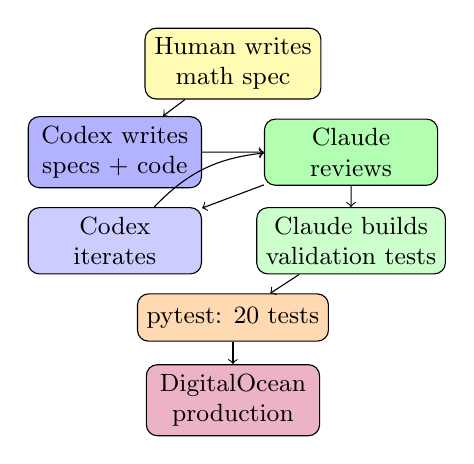
\begin{tikzpicture}[scale=0.75,
    box/.style={rectangle, draw, rounded corners, minimum width=2.2cm, minimum height=0.6cm, align=center, font=\small}]

    \node[box, fill=yellow!30] (human) at (0,4) {Human writes\\math spec};
    \node[box, fill=blue!30] (codex1) at (-2,2.5) {Codex writes\\specs + code};
    \node[box, fill=green!30] (claude1) at (2,2.5) {Claude\\reviews};
    \node[box, fill=blue!20] (codex2) at (-2,1) {Codex\\iterates};
    \node[box, fill=green!20] (claude2) at (2,1) {Claude builds\\validation tests};
    \node[box, fill=orange!30] (pytest) at (0,-0.3) {pytest: 20 tests};
    \node[box, fill=purple!30] (deploy) at (0,-1.7) {DigitalOcean\\production};

    \draw[->] (human) -- (codex1);
    \draw[->] (codex1) -- (claude1);
    \draw[->] (claude1) -- (codex2);
    \draw[->] (claude1) -- (claude2);
    \draw[->] (codex2) to[bend left=20] (claude1);
    \draw[->] (claude2) -- (pytest);
    \draw[->] (pytest) -- (deploy);
\end{tikzpicture}
\end{center}

\textbf{Iteration:} Multiple cycles until all 20 tests pass
\end{frame}

\begin{frame}{Zero-Intervention Automation Pipeline}
\textbf{A Hobby Project with Production-Grade Rigor:}

One prompt triggers the \textbf{entire pipeline} --- no human intervention:

\begin{enumerate}
    \item \textcolor{blue!70}{\textbf{Coding}} --- AI implements from specs
    \item \textcolor{orange!70}{\textbf{Regression Testing}} --- pytest runs 20+ tests locally
    \item \textcolor{purple!70}{\textbf{Browser UI Testing}} --- Playwright validates Flask UI
    \item \textcolor{green!70}{\textbf{Documentation}} --- LaTeX auto-updated
    \item \textcolor{cyan!70}{\textbf{Deploy to DigitalOcean}} --- SSH + Git + systemd
    \item \textcolor{orange!70}{\textbf{Production Regression}} --- Tests on live server
    \item \textcolor{red!70}{\textbf{Telegram Notification}} --- ``Done!''
\end{enumerate}

\vspace{0.2cm}
\begin{center}
\fbox{\parbox{0.85\textwidth}{
\textbf{Key Insight:} \$7/month hobby project built with the same rigor as top tech company production systems.
}}
\end{center}
\end{frame}

\begin{frame}{QuantLib Extension Strategy}
\textbf{QuantLib's Limitations:}
\begin{itemize}
    \item No native callable XCCY support
    \item Limited multi-currency Monte Carlo
    \item No built-in LSM for cross-currency
\end{itemize}

\textbf{How We Extended It (Collaboratively):}
\begin{enumerate}
    \item \textbf{Human:} Defined what QuantLib provides vs what's needed
    \item \textbf{Codex:} Wrote custom Monte Carlo using QuantLib curves
    \item \textbf{Claude:} Verified QuantLib API usage against docs
    \item \textbf{Stack Overflow:} Confirmed edge cases and patterns
\end{enumerate}

\textbf{Result:}
\begin{itemize}
    \item Use QuantLib for: curves, dates, calendars, basic calibration
    \item Custom code for: multi-factor MC, LSM, XCCY cashflows
    \item 1,400+ lines of rigorous extensions
\end{itemize}
\end{frame}

\begin{frame}[fragile]{DigitalOcean Deployment: Detailed Steps}
\textbf{1. Droplet Creation (DigitalOcean Console):}
\begin{itemize}
    \item Region: NYC3 or SFO3 for US users
    \item Image: Ubuntu 22.04 LTS
    \item Plan: Basic \$7/month (2GB RAM, 1 vCPU) --- hobby-friendly!
    \item Authentication: SSH key (not password)
\end{itemize}

\textbf{2. Initial Server Setup:}
\begin{verbatim}
ssh root@your-droplet-ip
apt update && apt upgrade -y
adduser deploy
usermod -aG sudo deploy
\end{verbatim}

\textbf{3. Application Deployment:}
\begin{verbatim}
cd /opt && git clone <repo>
python3 -m venv .venv
.venv/bin/pip install -r requirements.txt
cp deploy/systemd/*.template /etc/systemd/system/
systemctl enable --now tgir-quantlib-tools
\end{verbatim}
\end{frame}

\begin{frame}[fragile]{DigitalOcean: SSL and Apache Configuration}
\textbf{Apache Setup:}
\begin{verbatim}
apt install apache2
a2enmod proxy proxy_http ssl rewrite
cp deploy/apache/*.template /etc/apache2/sites-available/
a2ensite tgir-quantlib-tools
systemctl reload apache2
\end{verbatim}

\textbf{SSL with Certbot:}
\begin{verbatim}
apt install certbot python3-certbot-apache
certbot --apache -d your-domain.com
\end{verbatim}

\textbf{Firewall:}
\begin{verbatim}
ufw allow 22/tcp
ufw allow 80/tcp
ufw allow 443/tcp
ufw enable
\end{verbatim}

\textbf{Result:} HTTPS-secured Flask app at \texttt{https://your-domain.com}
\end{frame}

\begin{frame}{Why Codex + Claude Collaboration Works}
\textbf{Complementary Strengths:}
\begin{itemize}
    \item \textbf{Codex:} Excellent at ground-up implementation from specs
    \item \textbf{Claude:} Excellent at review, validation, extension
    \item \textbf{Human:} Domain expertise, orchestration, final judgment
\end{itemize}

\textbf{Error Detection:}
\begin{itemize}
    \item Claude catches bugs in Codex's implementations
    \item Codex fixes issues Claude identifies
    \item Neither alone would produce same quality
\end{itemize}

\textbf{Stack Overflow Role:}
\begin{itemize}
    \item AI can hallucinate APIs that don't exist
    \item Human experts catch edge cases
    \item Community validates approaches
\end{itemize}

\textbf{Key Lesson:}\\[0.2cm]
\fbox{\parbox{0.85\textwidth}{\centering Two AI agents + human domain expert\\produces better results than any single agent}}
\end{frame}

\begin{frame}{The Methodology IS the Innovation}
\textbf{This project delivers TWO things:}

\begin{enumerate}
    \item \textbf{Callable XCCY Pricer:}
    \begin{itemize}
        \item Three-factor Monte Carlo
        \item Longstaff-Schwartz optimization
        \item 20 validation tests
        \item Production deployment
    \end{itemize}

    \item \textbf{Collaborative Development Methodology:}
    \begin{itemize}
        \item Human $\to$ Codex (specs, implementation)
        \item Codex $\to$ Claude (review, validation)
        \item Claude $\to$ Regression tests (future-proofing)
        \item Full ecosystem: Mac + DigitalOcean + QuantLib + Python
    \end{itemize}
\end{enumerate}

\vspace{0.3cm}
\textbf{The methodology is reusable for other complex pricers}

\fbox{\parbox{0.85\textwidth}{\centering The collaborative workflow is as valuable as the callable XCCY pricer itself}}
\end{frame}

\begin{frame}{Reusable Human-Agent Development Pattern}
\begin{center}
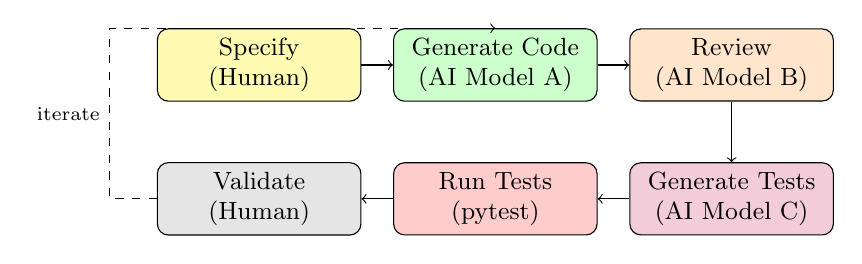
\begin{tikzpicture}[
    box/.style={rectangle, draw, rounded corners, text width=2.35cm, minimum height=0.9cm, align=center, font=\small}]
    \node[box, fill=yellow!30] (spec) at (-3,2.4) {Specify\\(Human)};
    \node[box, fill=green!20] (gen) at (0,2.4) {Generate Code\\(AI Model A)};
    \node[box, fill=orange!20] (review) at (3,2.4) {Review\\(AI Model B)};
    \node[box, fill=purple!20] (test) at (3,0.7) {Generate Tests\\(AI Model C)};
    \node[box, fill=red!20] (run) at (0,0.7) {Run Tests\\(pytest)};
    \node[box, fill=gray!20] (valid) at (-3,0.7) {Validate\\(Human)};

    \draw[->] (spec) -- (gen);
    \draw[->] (gen) -- (review);
    \draw[->] (review) -- (test);
    \draw[->] (test) -- (run);
    \draw[->] (run) -- (valid);
    \draw[->, dashed] (valid.west) -- ++(-0.6,0) |- node[pos=0.25,left,font=\scriptsize] {iterate} (gen.north);
\end{tikzpicture}
\end{center}

\textbf{Key Principle:}\\[0.3cm]
\fbox{\parbox{0.85\textwidth}{\centering Human provides specifications and validation\\AI accelerates implementation and review}}
\end{frame}

\begin{frame}{}
\begin{center}
\Huge\textbf{End of Supplementary Material}\\[2cm]
\Large Return to Main Presentation
\end{center}
\end{frame}

\end{document}

% Or compile separately

\documentclass[aspectratio=169,11pt]{beamer}
\usepackage[T1]{fontenc}
\usepackage[utf8]{inputenc}
\usepackage{lmodern}
\usepackage{mastering_ir_derivatives_beamer_1.0}
\usepackage{booktabs}
\usepackage{array}
\usepackage{listings}

% Retain the supplied visual system without changing the authored slide count.
\beamerdefaultoverlayspecification{<*>}
\AtBeginSection[]{}
\AtBeginSubsection[]{}

\hypersetup{
    colorlinks=true,
    linkcolor=blue,
    urlcolor=blue
}

\lstset{
    basicstyle=\ttfamily\scriptsize,
    breaklines=true,
    columns=fullflexible
}

\newcommand{\product}{TGIR QuantLib Tools}
\newcommand{\code}[1]{\texttt{#1}}
\newcommand{\docdate}{2026-04-06}


\usepackage[utf8]{inputenc}
\usepackage{amsmath,amssymb}
\usepackage{booktabs}
\usepackage{multirow}
\usepackage{listings}
\usepackage{tikz}
\usepackage{xcolor}

\lstset{
    language=Python,
    basicstyle=\ttfamily\scriptsize,
    keywordstyle=\color{blue}\bfseries,
    commentstyle=\color{green!50!black},
    stringstyle=\color{red},
    showstringspaces=false,
    breaklines=true,
    frame=single,
    backgroundcolor=\color{gray!10}
}

\title[Supplementary Content]{\textbf{QuantLib Derivatives Pricing}\\Supplementary Technical Slides}
\author{Quantitative Analytics Team}
\date{August 2026}

\begin{document}

%%%%%%%%%%%%%%%%%%%%%%%%%%%%%%%%%%%%%%%%%%%%%%%%%%%%%%%%%%%%%%%%%%%%%%%%%%%%%%%%
%% APPENDIX A: MATHEMATICAL FOUNDATIONS (20 slides)
%%%%%%%%%%%%%%%%%%%%%%%%%%%%%%%%%%%%%%%%%%%%%%%%%%%%%%%%%%%%%%%%%%%%%%%%%%%%%%%%

\begin{frame}
\titlepage
\end{frame}

\begin{frame}{}
\begin{center}
\Huge\textbf{Appendix A}\\[1cm]
\Large Mathematical Foundations\\[0.5cm]
\normalsize Stochastic Calculus Essentials
\end{center}
\end{frame}

\begin{frame}{Brownian Motion: Definition}
\begin{block}{Standard Brownian Motion $W_t$}
A stochastic process with:
\begin{enumerate}
    \item $W_0 = 0$
    \item Independent increments: $W_t - W_s \perp W_s - W_u$ for $t > s > u$
    \item Normally distributed: $W_t - W_s \sim N(0, t-s)$
    \item Continuous paths
\end{enumerate}
\end{block}

\textbf{Key Properties:}
\begin{itemize}
    \item $\mathbb{E}[W_t] = 0$
    \item $\text{Var}[W_t] = t$
    \item $\mathbb{E}[W_t W_s] = \min(t, s)$
    \item Paths are nowhere differentiable
\end{itemize}
\end{frame}

\begin{frame}{Itô's Lemma}
\begin{block}{Itô's Formula}
For $f(t, X_t)$ where $dX_t = \mu\,dt + \sigma\,dW_t$:
\[
df = \frac{\partial f}{\partial t}dt + \frac{\partial f}{\partial x}dX_t + \frac{1}{2}\frac{\partial^2 f}{\partial x^2}\sigma^2 dt
\]
\end{block}

\textbf{Example: Geometric Brownian Motion}

Let $S_t$ follow $dS_t = \mu S_t\,dt + \sigma S_t\,dW_t$. Apply Itô to $f(S) = \ln S$:
\[
d\ln S = \frac{1}{S}dS - \frac{1}{2}\frac{1}{S^2}\sigma^2 S^2 dt = \left(\mu - \frac{\sigma^2}{2}\right)dt + \sigma\,dW_t
\]

Therefore: $S_T = S_0 \exp\left[(\mu - \frac{\sigma^2}{2})T + \sigma W_T\right]$
\end{frame}

\begin{frame}{Risk-Neutral Pricing}
\begin{block}{Fundamental Theorem of Asset Pricing}
No-arbitrage $\Leftrightarrow$ Exists a probability measure $\mathbb{Q}$ such that discounted asset prices are martingales.
\end{block}

\textbf{Pricing Formula:}
\[
V_0 = \mathbb{E}^\mathbb{Q}\left[e^{-\int_0^T r_s\,ds} \cdot \text{Payoff}_T\right]
\]

\textbf{Change of Measure (Girsanov):}
\begin{itemize}
    \item Under $\mathbb{P}$: $dS = \mu S\,dt + \sigma S\,dW^\mathbb{P}$
    \item Under $\mathbb{Q}$: $dS = r S\,dt + \sigma S\,dW^\mathbb{Q}$
    \item $dW^\mathbb{Q} = dW^\mathbb{P} + \frac{\mu - r}{\sigma}dt$
\end{itemize}
\end{frame}

\begin{frame}{Ornstein-Uhlenbeck Process}
\begin{block}{OU Process}
\[
dx_t = -a x_t\,dt + \sigma\,dW_t
\]
\end{block}

\textbf{Solution:}
\[
x_t = x_0 e^{-at} + \sigma \int_0^t e^{-a(t-s)}\,dW_s
\]

\textbf{Properties:}
\begin{itemize}
    \item Mean: $\mathbb{E}[x_t] = x_0 e^{-at}$
    \item Variance: $\text{Var}[x_t] = \frac{\sigma^2}{2a}(1 - e^{-2at})$
    \item Stationary distribution: $N(0, \frac{\sigma^2}{2a})$
    \item Auto-correlation: $\text{Corr}(x_t, x_s) = e^{-a|t-s|}$
\end{itemize}

\textbf{Hull-White:} Add time-dependent mean $\theta(t)$
\end{frame}

\begin{frame}{Affine Term Structure Models}
\begin{block}{Affine Property}
Discount bond prices have the form:
\[
P(t, T) = e^{A(t,T) - B(t,T) r_t}
\]
\end{block}

\textbf{For Hull-White:}
\[
B(t, T) = \frac{1 - e^{-a(T-t)}}{a}
\]
\[
A(t, T) = \int_t^T \theta(s) B(s, T)\,ds - \frac{\sigma^2}{2}\int_t^T B(s, T)^2\,ds
\]

\textbf{Implications:}
\begin{itemize}
    \item Analytical bond and swaption prices
    \item Efficient calibration
    \item Foundation for tree methods
\end{itemize}
\end{frame}

\begin{frame}{Multi-Factor Models: Correlated Brownians}
\textbf{Correlated Brownian Motions:}

Given correlation matrix $\mathbf{R}$, generate correlated increments:
\[
\begin{pmatrix} dW_1 \\ dW_2 \\ dW_3 \end{pmatrix} = \mathbf{L} \cdot \begin{pmatrix} dZ_1 \\ dZ_2 \\ dZ_3 \end{pmatrix}
\]

Where $\mathbf{L}$ is the Cholesky decomposition: $\mathbf{R} = \mathbf{L}\mathbf{L}^T$

\textbf{Example:} $\rho_{12} = 0.25$, $\rho_{13} = -0.15$, $\rho_{23} = -0.30$

\[
\mathbf{L} = \begin{pmatrix}
1 & 0 & 0 \\
0.25 & 0.968 & 0 \\
-0.15 & -0.271 & 0.951
\end{pmatrix}
\]
\end{frame}

\begin{frame}{Variance Calculation for Joint Processes}
\textbf{For state $\mathbf{x}_t$:}
\[
\text{Cov}[\mathbf{x}_{t+h}, \mathbf{x}_{t+h}] = \int_0^h \mathbf{K}(s) \cdot \mathbf{R} \cdot \mathbf{K}(s)^T\,ds
\]

Where $\mathbf{K}(s)$ is the kernel matrix mapping Brownians to state.

\textbf{Numerical Integration:}
\[
\int_0^h f(s)\,ds \approx \frac{h}{2}\sum_{i=1}^{n} w_i f\left(\frac{h}{2}(x_i + 1)\right)
\]

Using Gauss-Legendre nodes $x_i$ and weights $w_i$.

\textbf{Our Implementation:} 16-point Gauss-Legendre quadrature
\end{frame}

\begin{frame}{Change of Numéraire}
\begin{block}{Numéraire Change}
When changing from numéraire $N_1$ to $N_2$:
\[
\frac{d\mathbb{Q}^{N_2}}{d\mathbb{Q}^{N_1}}\bigg|_{\mathcal{F}_T} = \frac{N_2(T) / N_2(0)}{N_1(T) / N_1(0)}
\]
\end{block}

\textbf{FX Pricing Application:}

Under USD money-market measure:
\begin{itemize}
    \item USD bank account is numéraire
    \item EUR rates get quanto adjustment
    \item FX drift includes rate differential
\end{itemize}

\[
d\ln X = (r^{USD} - r^{EUR} - \tfrac{1}{2}\sigma_X^2)\,dt + \sigma_X\,dW_X
\]
\end{frame}

\begin{frame}{Quanto Adjustment Derivation}
\textbf{Setting:} Price a EUR asset $S^{EUR}$ from USD perspective

\textbf{Under EUR measure:}
\[
dS^{EUR} = r^{EUR} S^{EUR}\,dt + \sigma_S S^{EUR}\,dW_S^{EUR}
\]

\textbf{Converting to USD measure:}
\[
dS^{EUR} = (r^{EUR} - \rho_{S,X}\sigma_S\sigma_X) S^{EUR}\,dt + \sigma_S S^{EUR}\,dW_S^{USD}
\]

\textbf{Intuition:}
\begin{itemize}
    \item If $\rho_{S,X} > 0$: Asset rises when EUR appreciates
    \item Extra expected USD return from FX
    \item Must subtract to stay risk-neutral
\end{itemize}
\end{frame}

%%%%%%%%%%%%%%%%%%%%%%%%%%%%%%%%%%%%%%%%%%%%%%%%%%%%%%%%%%%%%%%%%%%%%%%%%%%%%%%%
%% APPENDIX B: QUANTLIB DEEP DIVE (20 slides)
%%%%%%%%%%%%%%%%%%%%%%%%%%%%%%%%%%%%%%%%%%%%%%%%%%%%%%%%%%%%%%%%%%%%%%%%%%%%%%%%

\begin{frame}{}
\begin{center}
\Huge\textbf{Appendix B}\\[1cm]
\Large QuantLib Deep Dive\\[0.5cm]
\normalsize Internal Architecture and APIs
\end{center}
\end{frame}

\begin{frame}{QuantLib Class Hierarchy}
\begin{center}
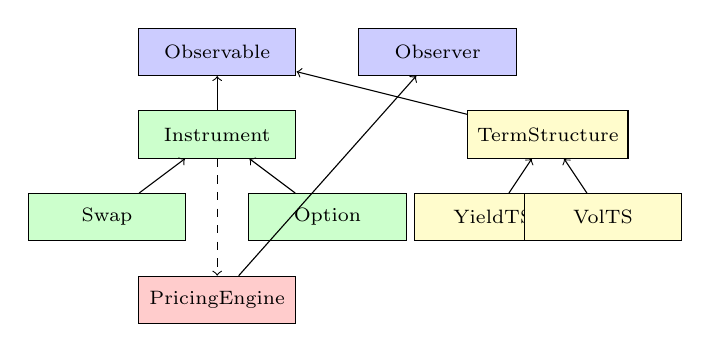
\begin{tikzpicture}[scale=0.7,
    box/.style={rectangle, draw, minimum width=2cm, minimum height=0.6cm, font=\scriptsize}]

    % Observer pattern
    \node[box, fill=blue!20] (obs) at (0,4) {Observable};
    \node[box, fill=blue!20] (obsr) at (4,4) {Observer};

    % Instruments
    \node[box, fill=green!20] (inst) at (0,2.5) {Instrument};
    \node[box, fill=green!20] (swap) at (-2,1) {Swap};
    \node[box, fill=green!20] (opt) at (2,1) {Option};

    % Term structures
    \node[box, fill=yellow!20] (ts) at (6,2.5) {TermStructure};
    \node[box, fill=yellow!20] (yts) at (5,1) {YieldTS};
    \node[box, fill=yellow!20] (vts) at (7,1) {VolTS};

    % Engines
    \node[box, fill=red!20] (eng) at (0,-0.5) {PricingEngine};

    \draw[->] (inst) -- (obs);
    \draw[->] (swap) -- (inst);
    \draw[->] (opt) -- (inst);
    \draw[->] (ts) -- (obs);
    \draw[->] (yts) -- (ts);
    \draw[->] (vts) -- (ts);
    \draw[->] (eng) -- (obsr);
    \draw[dashed,->] (inst) -- (eng);
\end{tikzpicture}
\end{center}

\textbf{Key Patterns:}
\begin{itemize}
    \item Observer/Observable for lazy evaluation
    \item Instruments are priced by Engines
    \item Term structures hold market data
\end{itemize}
\end{frame}

\begin{frame}[fragile]{Date and Calendar Handling}
\begin{lstlisting}[language=Python]
import QuantLib as ql

# Date construction
d1 = ql.Date(15, 8, 2026)           # Day, Month, Year
d2 = ql.Date(15, ql.August, 2026)   # Using enum
d3 = ql.DateParser.parseISO("2026-08-15")

# Date arithmetic
d4 = d1 + ql.Period(3, ql.Months)
d5 = d1 + 30  # Add 30 calendar days

# Calendar operations
cal = ql.UnitedStates(ql.UnitedStates.Settlement)
if cal.isBusinessDay(d1):
    print("Business day")

# Advance by business days
spot = cal.advance(d1, 2, ql.Days)

# Joint calendar (requires both to be open)
joint = ql.JointCalendar(ql.TARGET(),
    ql.UnitedStates(ql.UnitedStates.Settlement),
    ql.JoinHolidays)
\end{lstlisting}
\end{frame}

\begin{frame}[fragile]{Index Classes}
\begin{lstlisting}[language=Python]
# Overnight indices
sofr = ql.Sofr()
estr = ql.Estr()
sonia = ql.Sonia()

# Link to curve
curve_handle = ql.YieldTermStructureHandle(curve)
sofr_with_curve = ql.Sofr(curve_handle)

# Get fixings
fixing_date = ql.Date(10, 8, 2026)
rate = sofr.fixing(fixing_date)

# Add historical fixings (for backward-looking)
ql.IndexManager.instance().clearHistories()
sofr.addFixing(ql.Date(1, 8, 2026), 0.04)
sofr.addFixing(ql.Date(2, 8, 2026), 0.0402)
\end{lstlisting}
\end{frame}

\begin{frame}[fragile]{Yield Curve Construction Details}
\begin{lstlisting}[language=Python]
# Rate helpers
helpers = []

# Deposit helper (for short end)
helpers.append(ql.DepositRateHelper(
    ql.QuoteHandle(ql.SimpleQuote(0.041)),  # Rate
    ql.Period(1, ql.Days),                   # Tenor
    0,                                        # Settlement days
    ql.UnitedStates(ql.UnitedStates.Settlement),
    ql.ModifiedFollowing,                    # Convention
    False,                                   # End of month
    ql.Actual360()                          # Day count
))

# OIS helpers
for tenor, rate in [("1Y", 0.039), ("5Y", 0.037)]:
    helpers.append(ql.OISRateHelper(
        2, ql.Period(tenor),
        ql.QuoteHandle(ql.SimpleQuote(rate)),
        ql.Sofr()
    ))

# Build curve
curve = ql.PiecewiseLogLinearDiscount(today, helpers, ql.Actual365Fixed())
curve.enableExtrapolation()
\end{lstlisting}
\end{frame}

\begin{frame}[fragile]{OvernightIndexedSwap Instrument}
\begin{lstlisting}[language=Python]
# Create OIS swap
schedule = ql.Schedule(
    start_date, end_date,
    ql.Period(ql.Semiannual),          # Payment frequency
    calendar,
    ql.ModifiedFollowing,              # Business day convention
    ql.ModifiedFollowing,
    ql.DateGeneration.Backward,
    False                              # End of month
)

swap = ql.OvernightIndexedSwap(
    ql.Swap.Payer,                     # Type
    100_000_000.0,                     # Notional
    schedule,
    0.04,                              # Fixed rate
    ql.Actual360(),                    # Fixed day count
    ql.Sofr(curve_handle),             # Index
    0.0,                               # Spread on floating
    0,                                 # Payment lag
    ql.ModifiedFollowing,
    calendar
)
\end{lstlisting}
\end{frame}

\begin{frame}[fragile]{Swaption Construction}
\begin{lstlisting}[language=Python]
# Create underlying swap
underlying = ql.VanillaSwap(
    ql.Swap.Payer, notional,
    fixed_schedule, strike, day_count,
    float_schedule, sofr_index, 0.0, day_count
)

# European exercise
expiry = ql.Date(15, 8, 2028)
exercise = ql.EuropeanExercise(expiry)

# Bermudan exercise
call_dates = [ql.Date(15, 8, 2028 + i) for i in range(5)]
exercise = ql.BermudanExercise(call_dates)

# Create swaption
swaption = ql.Swaption(underlying, exercise)

# Set pricing engine
engine = ql.TreeSwaptionEngine(hw_model, 50)
swaption.setPricingEngine(engine)

print(f"NPV: {swaption.NPV():,.2f}")
\end{lstlisting}
\end{frame}

\begin{frame}[fragile]{Hull-White Model Setup}
\begin{lstlisting}[language=Python]
# Create model with fixed parameters
mean_reversion = 0.03
volatility = 0.01
model = ql.HullWhite(curve_handle, mean_reversion, volatility)

# Get model parameters
params = model.params()
print(f"a = {params[0]}, sigma = {params[1]}")

# Create calibration helpers
helpers = []
for expiry, tenor, vol_bp in [("2Y", "8Y", 78), ("5Y", "5Y", 80)]:
    helper = ql.SwaptionHelper(
        ql.Period(expiry), ql.Period(tenor),
        ql.QuoteHandle(ql.SimpleQuote(vol_bp * 1e-4)),
        sofr_index, ql.Period("1Y"), ql.Actual360(),
        ql.Actual360(), curve_handle,
        ql.BlackCalibrationHelper.RelativePriceError,
        ql.nullDouble(), 1.0, ql.Normal
    )
    helper.setPricingEngine(ql.JamshidianSwaptionEngine(model))
    helpers.append(helper)
\end{lstlisting}
\end{frame}

\begin{frame}[fragile]{Model Calibration}
\begin{lstlisting}[language=Python]
# Calibration settings
opt_method = ql.LevenbergMarquardt()
end_criteria = ql.EndCriteria(
    500,    # Max iterations
    100,    # Max stationary
    1e-10,  # Root epsilon
    1e-10,  # Function epsilon
    1e-10   # Gradient epsilon
)

# Which parameters to calibrate
# [True, False] means calibrate a, keep sigma fixed
fixed_params = ql.BoolVector([True, False])

# Run calibration
model.calibrate(
    helpers,        # Calibration instruments
    opt_method,
    end_criteria,
    ql.PositiveConstraint(),  # Parameter constraint
    ql.DoubleVector(),        # Weights
    fixed_params
)

# Check results
print(f"Calibrated sigma: {model.params()[1]:.6f}")
\end{lstlisting}
\end{frame}

\begin{frame}[fragile]{Calibration Diagnostics}
\begin{lstlisting}[language=Python]
# After calibration, check fit quality
for i, helper in enumerate(helpers):
    market_val = helper.marketValue()
    model_val = helper.modelValue()
    error = (model_val - market_val) / market_val

    # Get implied vol
    impl_vol = helper.impliedVolatility(model_val, 1e-6, 100,
                                         1e-6, 2.0)

    print(f"Helper {i}:")
    print(f"  Market: {market_val:.6f}")
    print(f"  Model:  {model_val:.6f}")
    print(f"  Error:  {error*100:.3f}%")
    print(f"  Impl Vol: {impl_vol*10000:.1f}bp")

# Calculate weighted RMS
errors = [(h.modelValue()/h.marketValue() - 1)**2 for h in helpers]
rms = math.sqrt(sum(errors) / len(errors))
print(f"RMS Error: {rms*100:.3f}%")
\end{lstlisting}
\end{frame}

\begin{frame}{QuantLib Limitations for XCCY}
\textbf{Native XCCY Support:}
\begin{itemize}
    \item \texttt{CrossCurrencyBasisSwap} --- exists for vanilla XCCY
    \item \texttt{CrossCurrencyBasisSwapRateHelper} --- for curve building
    \item No native \textbf{callable} XCCY instrument
\end{itemize}

\textbf{Multi-Factor Limitations:}
\begin{itemize}
    \item Tree engines work for 1-2 factors
    \item No native 3-factor joint tree
    \item Would need FD solver on 3D grid (slow)
    \item Monte Carlo is natural choice
\end{itemize}

\textbf{Our Solution:}
\begin{itemize}
    \item Use QuantLib for curves, dates, indices
    \item Custom 3-factor Monte Carlo
    \item LSM for exercise optimization
\end{itemize}
\end{frame}

%%%%%%%%%%%%%%%%%%%%%%%%%%%%%%%%%%%%%%%%%%%%%%%%%%%%%%%%%%%%%%%%%%%%%%%%%%%%%%%%
%% APPENDIX C: MONTE CARLO METHODS (20 slides)
%%%%%%%%%%%%%%%%%%%%%%%%%%%%%%%%%%%%%%%%%%%%%%%%%%%%%%%%%%%%%%%%%%%%%%%%%%%%%%%%

\begin{frame}{}
\begin{center}
\Huge\textbf{Appendix C}\\[1cm]
\Large Monte Carlo Methods\\[0.5cm]
\normalsize Simulation Techniques and Variance Reduction
\end{center}
\end{frame}

\begin{frame}{Monte Carlo Basics}
\begin{block}{Law of Large Numbers}
\[
\frac{1}{N}\sum_{i=1}^{N} f(X_i) \xrightarrow{N\to\infty} \mathbb{E}[f(X)]
\]
\end{block}

\textbf{Standard Error:}
\[
SE = \frac{\sigma}{\sqrt{N}}
\]

\textbf{95\% Confidence Interval:}
\[
\bar{X} \pm 1.96 \times SE
\]

\textbf{Key Properties:}
\begin{itemize}
    \item Error decreases as $O(N^{-1/2})$
    \item Independent of dimension (curse of dimensionality avoided)
    \item Flexible for path-dependent payoffs
\end{itemize}
\end{frame}

\begin{frame}[fragile]{Random Number Generation}
\textbf{NumPy PCG64 Generator:}
\begin{itemize}
    \item Permuted Congruential Generator
    \item Period: $2^{128}$
    \item Excellent statistical properties
    \item Fast and reproducible
\end{itemize}

\textbf{Usage:}
\begin{lstlisting}[language=Python]
import numpy as np

# Create generator with seed
rng = np.random.Generator(np.random.PCG64(1729))

# Generate standard normals
Z = rng.standard_normal((paths, dimensions))
\end{lstlisting}

\textbf{Reproducibility:}
\begin{itemize}
    \item Same seed $\Rightarrow$ same sequence
    \item Critical for debugging and validation
\end{itemize}
\end{frame}

\begin{frame}[fragile]{Variance Reduction: Antithetic Variates}
\begin{block}{Antithetic Sampling}
If $\hat{\theta}_1 = f(Z)$ and $\hat{\theta}_2 = f(-Z)$ are negatively correlated, then:
\[
\text{Var}\left[\frac{\hat{\theta}_1 + \hat{\theta}_2}{2}\right] < \text{Var}[\hat{\theta}_1]
\]
\end{block}

\textbf{Implementation:}
\begin{lstlisting}[language=Python]
def antithetic_normals(rng, paths, dims):
    half = (paths + 1) // 2
    draws = rng.standard_normal((half, dims))
    return np.concatenate([draws, -draws])[:paths]
\end{lstlisting}

\textbf{Benefits:}
\begin{itemize}
    \item Forces mean of normals to be exactly 0
    \item Reduces variance for most payoffs
    \item No additional cost per sample
\end{itemize}
\end{frame}

\begin{frame}{Variance Reduction: Control Variates}
\begin{block}{Control Variate Method}
Use a correlated variable $Y$ with known mean $\mu_Y$:
\[
\hat{\theta}_{CV} = \hat{\theta} - \beta(\bar{Y} - \mu_Y)
\]
\end{block}

\textbf{Optimal $\beta$:}
\[
\beta^* = \frac{\text{Cov}[\hat{\theta}, Y]}{\text{Var}[Y]}
\]

\textbf{Applications in Derivatives:}
\begin{itemize}
    \item Use underlying asset as control
    \item Use European price for Bermudan
    \item Use delta-hedged portfolio
\end{itemize}
\end{frame}

\begin{frame}{Quasi-Monte Carlo (QMC)}
\textbf{Low-Discrepancy Sequences:}
\begin{itemize}
    \item Sobol, Halton, Niederreiter
    \item Fill space more uniformly than random
    \item Error $O(N^{-1})$ vs $O(N^{-1/2})$
\end{itemize}

\textbf{Trade-offs:}
\begin{itemize}
    \item Better for smooth integrands
    \item Dimension-dependent effectiveness
    \item Standard error not directly computable
\end{itemize}

\textbf{Not used in our implementation:}
\begin{itemize}
    \item Standard MC simpler to implement
    \item Antithetic sufficient for our accuracy needs
    \item QMC would be future enhancement
\end{itemize}
\end{frame}

\begin{frame}{Path Generation: Euler vs Exact}
\textbf{Euler Discretization:}
\[
x_{t+\Delta t} = x_t + \mu(x_t)\Delta t + \sigma(x_t)\sqrt{\Delta t}\, Z
\]

\textbf{Exact Simulation (OU process):}
\[
x_{t+h} = x_t e^{-ah} + \sigma\int_0^h e^{-a(h-s)}\,dW_s
\]

\textbf{Our Approach: Exact OU Kernels}
\begin{itemize}
    \item Hull-White factors use exact solution
    \item No discretization bias
    \item Larger time steps possible
    \item Covariance computed exactly
\end{itemize}
\end{frame}

\begin{frame}[fragile]{State Evolution Implementation}
\begin{lstlisting}[language=Python]
@dataclass
class StepTransition:
    matrix: np.ndarray      # Transition matrix A
    offset: np.ndarray      # Deterministic drift b
    covariance_root: np.ndarray  # sqrt(Sigma)

def evolve_state(state, transition, normals):
    """
    x_{t+h} = A * x_t + b + L * Z

    state: (paths, 5) current state
    transition: StepTransition object
    normals: (paths, 5) standard normals

    Returns: (paths, 5) new state
    """
    return (state @ transition.matrix.T
            + transition.offset
            + normals @ transition.covariance_root.T)
\end{lstlisting}
\end{frame}

\begin{frame}{Cash Flow Valuation}
\textbf{For each simulated path:}

\textbf{Fixed Cash Flow:}
\[
PV = \text{Amount} \times e^{-I_{USD}(t_{pay})}
\]

\textbf{Floating Cash Flow (compounded overnight):}
\[
\text{Amount} = N \times \left(e^{I_{EUR}(t_{end}) - I_{EUR}(t_{start}) + \text{basis}} - 1\right)
\]
\[
PV = \text{Amount} \times X_{t_{pay}} \times e^{-I_{USD}(t_{pay})}
\]

\textbf{FX Conversion:} EUR amounts converted at simulated FX rate

\textbf{Notional Exchanges:}
\begin{itemize}
    \item Initial: Net of notionals at spot
    \item Final: Net of notionals at terminal FX
\end{itemize}
\end{frame}

\begin{frame}{LSM: Basis Function Selection}
\textbf{State Variables:} $(x_{USD}, x_{EUR}, \ln X - \ln X_0)$

\textbf{Polynomial Basis (10 functions):}
\[
\phi = (1,\, x,\, y,\, z,\, x^2,\, y^2,\, z^2,\, xy,\, xz,\, yz)
\]

\textbf{Why This Choice?}
\begin{itemize}
    \item Captures main effects (linear terms)
    \item Captures curvature (squared terms)
    \item Captures interactions (cross terms)
    \item Low-dimensional (avoids overfitting)
\end{itemize}

\textbf{Alternatives:}
\begin{itemize}
    \item Laguerre polynomials
    \item Chebyshev polynomials
    \item Neural network approximation
\end{itemize}
\end{frame}

\begin{frame}{LSM: Numerical Stability}
\textbf{Problem: Ill-Conditioned Design Matrix}

When state variables have different scales or are correlated:
\[
\text{cond}(\mathbf{X}^T\mathbf{X}) \gg 1
\]

\textbf{Solutions:}
\begin{enumerate}
    \item \textbf{Standardization:}
    \[
    \tilde{x} = \frac{x - \bar{x}}{\sigma_x}
    \]

    \item \textbf{Ridge Regression:}
    \[
    \boldsymbol{\beta} = (\mathbf{X}^T\mathbf{X} + \lambda\mathbf{I})^{-1}\mathbf{X}^T\mathbf{y}
    \]
\end{enumerate}

\textbf{Our Implementation:}
\begin{itemize}
    \item Standardize state variables
    \item Use \texttt{np.linalg.lstsq} with rcond
    \item Fall back to ridge if cond $>$ 1e10
\end{itemize}
\end{frame}

\begin{frame}{LSM: Two-Pass Why It Matters}
\textbf{Single-Pass Bias:}
\begin{itemize}
    \item Training on same paths as pricing
    \item Exercise decision uses future information
    \item Results in upward bias (too high)
\end{itemize}

\textbf{Two-Pass Solution:}
\begin{enumerate}
    \item \textbf{Training Pass:} Learn policy on paths 1...N
    \item \textbf{Pricing Pass:} Apply policy on paths N+1...2N
\end{enumerate}

\textbf{Properties:}
\begin{itemize}
    \item Pricing paths are independent of training
    \item No look-ahead bias
    \item Result is a \textit{lower bound} on true value
\end{itemize}

\textbf{Why Lower Bound?}
\begin{itemize}
    \item Suboptimal exercise policy
    \item True optimal policy would give higher value
    \item Upper bound requires dual methods
\end{itemize}
\end{frame}

\begin{frame}{Convergence Diagnostics}
\textbf{Standard Error Analysis:}
\[
SE = \frac{\sigma}{\sqrt{N}}
\]

\textbf{Expected Behavior:}
\begin{itemize}
    \item Double paths $\Rightarrow$ SE reduces by $\sqrt{2}$
    \item 10x paths $\Rightarrow$ SE reduces by $\sqrt{10} \approx 3.16$
\end{itemize}

\textbf{Test Protocol:}
\begin{enumerate}
    \item Run with 10K paths, record SE
    \item Run with 40K paths, record SE
    \item Verify ratio $\approx$ 2.0
\end{enumerate}

\textbf{If Ratio is Wrong:}
\begin{itemize}
    \item Implementation bug
    \item Correlation between paths
    \item Numerical instability
\end{itemize}
\end{frame}

%%%%%%%%%%%%%%%%%%%%%%%%%%%%%%%%%%%%%%%%%%%%%%%%%%%%%%%%%%%%%%%%%%%%%%%%%%%%%%%%
%% APPENDIX D: TESTING AND VALIDATION (20 slides)
%%%%%%%%%%%%%%%%%%%%%%%%%%%%%%%%%%%%%%%%%%%%%%%%%%%%%%%%%%%%%%%%%%%%%%%%%%%%%%%%

\begin{frame}{}
\begin{center}
\Huge\textbf{Appendix D}\\[1cm]
\Large Testing and Validation\\[0.5cm]
\normalsize Ensuring Model Correctness
\end{center}
\end{frame}

\begin{frame}{Validation Philosophy}
\begin{block}{Trust, But Verify}
Every model component needs independent validation.
\end{block}

\textbf{Levels of Testing:}
\begin{enumerate}
    \item \textbf{Unit Tests:} Individual functions
    \item \textbf{Integration Tests:} Component interactions
    \item \textbf{Calibration Tests:} Market data fit
    \item \textbf{Model Tests:} Arbitrage conditions
    \item \textbf{Convergence Tests:} Numerical accuracy
    \item \textbf{Boundary Tests:} Edge cases
\end{enumerate}
\end{frame}

\begin{frame}{Martingale Testing: Theory}
\textbf{Under Risk-Neutral Measure:}

Discounted tradeable assets must be martingales:
\[
\mathbb{E}^\mathbb{Q}[e^{-\int_0^T r_s\,ds} \cdot A_T] = A_0
\]

\textbf{Test Assets:}
\begin{enumerate}
    \item \textbf{USD Zero Coupon:} $\mathbb{E}[e^{-\int r^{USD}}] = P^{USD}(0,T)$
    \item \textbf{EUR Zero in USD:} $\mathbb{E}[e^{-\int r^{USD}} X_T] = X_0 P^{EUR}_{eff}(0,T)$
    \item \textbf{EUR Bank Account:} $\mathbb{E}[e^{-\int r^{USD}} X_T e^{\int r^{EUR}}] = X_0$
\end{enumerate}

\textbf{Statistical Test:}
\[
z = \frac{\bar{X}_{MC} - \text{Target}}{SE_{MC}}
\]
Pass if $|z| < 3.5$ (approximate 99.95\% confidence)
\end{frame}

\begin{frame}{Monotonicity Testing}
\textbf{Economic Relationships That Must Hold:}

\begin{itemize}
    \item $\uparrow$ Volatility $\Rightarrow$ $\uparrow$ Option Value
    \item $\uparrow$ Non-call Period $\Rightarrow$ $\downarrow$ Option Value
    \item $\uparrow$ FX Spot (EUR/USD) $\Rightarrow$ $\uparrow$ EUR Leg Value
    \item $\uparrow$ Interest Rates $\Rightarrow$ $\downarrow$ Long Duration Value
\end{itemize}

\textbf{Test Protocol:}
\begin{enumerate}
    \item Price with base parameters
    \item Bump parameter in expected direction
    \item Verify price moves correctly
    \item Allow for MC noise (use confidence bounds)
\end{enumerate}
\end{frame}

\begin{frame}{Structural Bounds}
\textbf{Test 1: Option Value Non-Negative}
\[
V_{callable} \geq V_{non-callable}
\]

\textbf{Test 2: Callable Decomposition}
\[
V_{callable} = V_{non-callable} + V_{option}
\]

\textbf{Test 3: Option Less Than Notional}
\[
V_{option} < \text{Notional}
\]

\textbf{Test 4: Leg Consistency}
\[
V_{USD} + V_{EUR} = V_{non-callable}
\]

(Within Monte Carlo error)
\end{frame}

\begin{frame}[fragile]{Test Implementation Example}
\begin{lstlisting}[language=Python]
class TestStructuralBounds:
    """Test fundamental arbitrage bounds."""

    def test_callable_ge_non_callable(self, base_result):
        """Callable >= Non-callable."""
        callable_npv = base_result["valuation"]["callable_npv"]["mean"]
        non_callable = base_result["valuation"]["non_callable_npv"]["mean"]
        option = base_result["valuation"]["embedded_option_value"]["mean"]

        assert option >= 0, f"Option must be >= 0, got {option:,.2f}"

        # Check decomposition
        recomputed = non_callable + option
        assert abs(callable_npv - recomputed) < 1.0, (
            f"Callable ({callable_npv:,.2f}) != "
            f"Non-callable ({non_callable:,.2f}) + Option ({option:,.2f})"
        )
\end{lstlisting}
\end{frame}

\begin{frame}{Calibration Quality Checks}
\textbf{OIS Curve Bootstrap:}
\begin{itemize}
    \item Each input OIS rate should reprice to $<$0.01bp
    \item Interpolation should be smooth
    \item No negative forward rates
\end{itemize}

\textbf{Swaption Calibration:}
\begin{itemize}
    \item Individual error $<$5\% relative
    \item RMS error $<$5\%
    \item Model parameters in reasonable range
\end{itemize}

\textbf{FX Vol Calibration:}
\begin{itemize}
    \item Each ATM vol within 25bp
    \item Term structure monotonic
    \item Implied sigmas positive
\end{itemize}
\end{frame}

\begin{frame}{Edge Case Testing}
\textbf{Zero Correlation:}
\begin{itemize}
    \item Set all correlations to 0
    \item Model should still work
    \item Results should be sensible
\end{itemize}

\textbf{High Correlation:}
\begin{itemize}
    \item Set correlations to extreme (but valid) values
    \item Check positive semi-definiteness
    \item Verify no numerical issues
\end{itemize}

\textbf{ATM Swap:}
\begin{itemize}
    \item Price with swap at par
    \item Non-callable value near zero
    \item Option value dominates
\end{itemize}
\end{frame}

\begin{frame}{Regression Testing}
\textbf{Golden Reference:}
\begin{itemize}
    \item Store results from validated run
    \item Compare new runs against reference
    \item Flag any deviations
\end{itemize}

\textbf{What to Compare:}
\begin{itemize}
    \item Calibrated parameters
    \item NPV values (within MC noise)
    \item Exercise probabilities
    \item Greeks (if computed)
\end{itemize}

\textbf{When to Update Reference:}
\begin{itemize}
    \item Bug fixes that change results
    \item Model enhancements
    \item After thorough validation
\end{itemize}
\end{frame}

\begin{frame}{Performance Testing}
\textbf{Benchmarks:}
\begin{itemize}
    \item Full pricing: $<$15 seconds
    \item 30,000 paths, 10Y horizon
    \item MacBook M1/M2 baseline
\end{itemize}

\textbf{Bottlenecks:}
\begin{enumerate}
    \item Path simulation (main loop)
    \item Cash flow accumulation
    \item Regression (matrix operations)
\end{enumerate}

\textbf{Optimization Strategies:}
\begin{itemize}
    \item Vectorize all operations
    \item Minimize memory allocation
    \item Use efficient BLAS (via NumPy)
    \item Consider chunking for large N
\end{itemize}
\end{frame}

%%%%%%%%%%%%%%%%%%%%%%%%%%%%%%%%%%%%%%%%%%%%%%%%%%%%%%%%%%%%%%%%%%%%%%%%%%%%%%%%
%% APPENDIX E: PRACTICAL CONSIDERATIONS (20 slides)
%%%%%%%%%%%%%%%%%%%%%%%%%%%%%%%%%%%%%%%%%%%%%%%%%%%%%%%%%%%%%%%%%%%%%%%%%%%%%%%%

\begin{frame}{}
\begin{center}
\Huge\textbf{Appendix E}\\[1cm]
\Large Practical Considerations\\[0.5cm]
\normalsize Real-World Deployment Challenges
\end{center}
\end{frame}

\begin{frame}{Market Data Challenges}
\textbf{Data Sources:}
\begin{itemize}
    \item Bloomberg, Reuters
    \item Exchange feeds
    \item Broker quotes
\end{itemize}

\textbf{Data Quality Issues:}
\begin{itemize}
    \item Stale quotes
    \item Bid/ask spreads
    \item Missing data points
    \item Timezone differences
\end{itemize}

\textbf{Our Approach:}
\begin{itemize}
    \item JSON input files
    \item Placeholder/illustrative data
    \item Clear ``REPLACE'' markers
    \item Schema validation
\end{itemize}
\end{frame}

\begin{frame}{Collateral and Funding}
\textbf{CSA (Credit Support Annex):}
\begin{itemize}
    \item Determines collateral posting rules
    \item Affects discount curve choice
    \item USD CSA $\Rightarrow$ SOFR discounting
\end{itemize}

\textbf{Cross-Currency Collateral:}
\begin{itemize}
    \item EUR deal, USD collateral
    \item Creates ``effective'' EUR curve
    \item Different from native EUR curve
\end{itemize}

\textbf{Our Implementation:}
\begin{itemize}
    \item Build EUR effective curve from FX forwards
    \item Discount EUR flows at effective rate
    \item Maintain forecast/discount separation
\end{itemize}
\end{frame}

\begin{frame}{Model Risk Management}
\textbf{Key Risks:}
\begin{itemize}
    \item Calibration failure
    \item Parameter instability
    \item Numerical errors
    \item Assumption violations
\end{itemize}

\textbf{Mitigations:}
\begin{itemize}
    \item Tolerance thresholds
    \item Calibration acceptance flags
    \item Martingale diagnostics
    \item Limitation documentation
\end{itemize}

\textbf{Documentation:}
\begin{itemize}
    \item Model specification
    \item Validation report
    \item Known limitations
    \item Appropriate use guidance
\end{itemize}
\end{frame}

\begin{frame}{Greeks and Risk}
\textbf{Bump-and-Revalue:}
\begin{itemize}
    \item Shift input, reprice, compute difference
    \item Simple but expensive
    \item Need common random numbers
\end{itemize}

\textbf{Key Greeks:}
\begin{itemize}
    \item \textbf{Delta:} $\partial V / \partial \text{rates}$
    \item \textbf{Vega:} $\partial V / \partial \text{vol}$
    \item \textbf{FX Delta:} $\partial V / \partial X$
    \item \textbf{Correlation:} $\partial V / \partial \rho$
\end{itemize}

\textbf{Not Implemented Yet:}
\begin{itemize}
    \item Pathwise derivatives
    \item Likelihood ratio method
    \item AAD (automatic differentiation)
\end{itemize}
\end{frame}

\begin{frame}{Performance Optimization}
\textbf{Current Performance:}
\begin{itemize}
    \item 30K paths: $\sim$10 seconds
    \item 100K paths: $\sim$30 seconds
    \item Acceptable for research
\end{itemize}

\textbf{Potential Improvements:}
\begin{enumerate}
    \item \textbf{Numba JIT:} Compile hot loops
    \item \textbf{CuPy:} GPU acceleration
    \item \textbf{Cython:} C extensions
    \item \textbf{C++ Port:} Full rewrite
\end{enumerate}

\textbf{Trade-offs:}
\begin{itemize}
    \item Development time vs runtime
    \item Maintainability
    \item Debugging complexity
\end{itemize}
\end{frame}

\begin{frame}{Production Readiness Checklist}
\textbf{Before Production Use:}
\begin{enumerate}
    \item[$\square$] Independent model review
    \item[$\square$] Dual/upper bound implementation
    \item[$\square$] Full market data integration
    \item[$\square$] Greeks computation
    \item[$\square$] Audit trail
    \item[$\square$] Error handling review
    \item[$\square$] Performance testing
    \item[$\square$] Security audit
    \item[$\square$] Documentation complete
    \item[$\square$] Regulatory approval
\end{enumerate}

\textbf{Current Status:} Research/educational use only
\end{frame}

\begin{frame}{Lessons Learned}
\begin{enumerate}
    \item \textbf{Start Simple:} Build vanilla first, then exotic

    \item \textbf{Validate Early:} Test each component before integration

    \item \textbf{Document Assumptions:} Future you will forget

    \item \textbf{Use QuantLib:} Don't reinvent dates, calendars, curves

    \item \textbf{Vectorize:} NumPy is your friend

    \item \textbf{Test Extensively:} Martingales, bounds, convergence

    \item \textbf{Accept Limitations:} No model is perfect
\end{enumerate}
\end{frame}

\begin{frame}{Resources and References}
\textbf{Books:}
\begin{itemize}
    \item Brigo \& Mercurio: ``Interest Rate Models''
    \item Glasserman: ``Monte Carlo Methods in Financial Engineering''
    \item Longstaff \& Schwartz (2001): LSM Paper
\end{itemize}

\textbf{QuantLib:}
\begin{itemize}
    \item \url{https://www.quantlib.org}
    \item \url{https://github.com/lballabio/QuantLib}
    \item \url{https://quantlib-python-docs.readthedocs.io}
\end{itemize}

\textbf{This Project:}
\begin{itemize}
    \item Repository: \texttt{tgir\_quantlib\_tools}
    \item Model ID: \texttt{HW1F\_USD\_HW1F\_EUR\_BSFX\_LSM\_V1}
\end{itemize}
\end{frame}

\begin{frame}{}
\begin{center}
\Huge\textbf{Appendix F}\\[1cm]
\Large Collaborative AI Development\\[0.5cm]
\normalsize Human + Codex + Claude + Tools
\end{center}
\end{frame}

%%%%%%%%%%%%%%%%%%%%%%%%%%%%%%%%%%%%%%%%%%%%%%%%%%%%%%%%%%%%%%%%%%%%%%%%%%%%%%%%
%% APPENDIX F: COLLABORATIVE AI DEVELOPMENT
%%%%%%%%%%%%%%%%%%%%%%%%%%%%%%%%%%%%%%%%%%%%%%%%%%%%%%%%%%%%%%%%%%%%%%%%%%%%%%%%

\begin{frame}{The Collaborative Development Model}
\textbf{This project demonstrates a new development paradigm:}

\begin{center}
\fbox{\parbox{0.85\textwidth}{\centering
\textbf{Human Domain Expert} (orchestrator)\\
$\downarrow$\\
\textbf{Codex} (specs, core programming, tests)\\
$\downarrow$\\
\textbf{Claude} (review, validation framework, extensions)\\
$\downarrow$\\
\textbf{Production System} (Mac + DigitalOcean)
}}
\end{center}

\vspace{0.5cm}
\textbf{Key Insight:}\\
The collaborative methodology is \textbf{as significant as the callable XCCY pricer itself}

\textbf{Reproducible Pattern:} Same workflow can build other complex pricers
\end{frame}

\begin{frame}{Division of Labor: Two AI Agents}
\begin{table}
\centering
\small
\begin{tabular}{p{3cm}p{4cm}p{4cm}}
\toprule
& \textbf{Codex (OpenAI)} & \textbf{Claude (Anthropic)} \\
\midrule
\textbf{Primary Role} & Core development & Review \& validation \\
\midrule
\textbf{Specs} & Wrote formal specifications & Reviewed for completeness \\
\textbf{Implementation} & Built Monte Carlo engine & Reviewed for correctness \\
\textbf{Tests} & Created initial test suite & Built validation framework \\
\textbf{Extensions} & --- & Extended with regression tests \\
\bottomrule
\end{tabular}
\end{table}

\textbf{Human Role:}
\begin{itemize}
    \item Provided domain expertise (financial mathematics)
    \item Orchestrated agent collaboration
    \item Final validation against theory
    \item Verified with Stack Overflow guidance
\end{itemize}
\end{frame}

\begin{frame}{Codex: Ground-Up Development}
\textbf{What Codex Built from Human Guidance:}

\begin{enumerate}
    \item \textbf{Rigorous Specifications:}
    \begin{itemize}
        \item Mathematical model documentation (LaTeX)
        \item API contracts with type hints
        \item JSON schemas for market data and trades
    \end{itemize}

    \item \textbf{Core Implementation:}
    \begin{itemize}
        \item Three-factor Monte Carlo (1,400+ lines)
        \item Longstaff-Schwartz regression
        \item SOFR/ESTR curve bootstrapping
        \item QuantLib integration layer
    \end{itemize}

    \item \textbf{Initial Test Suite:}
    \begin{itemize}
        \item Unit tests for each component
        \item Integration tests for pricing
        \item Smoke tests for API
    \end{itemize}
\end{enumerate}

\textbf{Human provided:} Math formulas, market conventions, QuantLib patterns
\end{frame}

\begin{frame}{Claude: Review and Validation Framework}
\textbf{Claude's Key Contributions:}

\begin{enumerate}
    \item \textbf{Code Review:}
    \begin{itemize}
        \item Reviewed all Codex implementations
        \item Identified numerical stability issues
        \item Suggested vectorization optimizations
    \end{itemize}

    \item \textbf{Validation Framework (Critical):}
    \begin{itemize}
        \item Martingale test infrastructure
        \item Structural bounds verification
        \item Monotonicity checking
        \item Convergence analysis
    \end{itemize}

    \item \textbf{Extensions for Regression:}
    \begin{itemize}
        \item Built tests to catch future changes
        \item Automated validation on every commit
        \item Documentation and lecture generation
    \end{itemize}
\end{enumerate}

\textbf{Result:} 20 automated tests that provide confidence in correctness
\end{frame}

\begin{frame}{The Full Technology Ecosystem}
\begin{table}
\centering
\small
\begin{tabular}{lll}
\toprule
\textbf{Layer} & \textbf{Component} & \textbf{Role} \\
\midrule
\multirow{2}{*}{Infrastructure} & Mac (local) & Development environment \\
 & DigitalOcean & Production hosting \\
\midrule
\multirow{3}{*}{AI Agents} & Codex (OpenAI) & Specs, core dev, tests \\
 & Claude (Anthropic) & Review, validation, docs \\
 & GitHub Copilot & Inline VS Code assistance \\
\midrule
\multirow{2}{*}{Libraries} & QuantLib (C++) & Curves, calibration \\
 & Python/NumPy & Simulation, Flask \\
\midrule
Resources & Stack Overflow & Guidance verification \\
\bottomrule
\end{tabular}
\end{table}

\textbf{Cohesion:} All components integrated in unified workflow
\end{frame}

\begin{frame}{Integration Boundaries: Proposed REST + Implemented MCP}
\textbf{Two Ways to Access the Pricer:}

\begin{table}
\centering
\small
\begin{tabular}{lll}
\toprule
\textbf{Interface} & \textbf{Use Case} & \textbf{Protocol} \\
\midrule
REST contract & Future trading system integration & HTTPS + JSON \\
 & (C++ clients, batch jobs) & Proposed /api/v1/ endpoints \\
\midrule
MCP Server & LLM integration & JSON-RPC \\
 & (Claude, GPT can call pricer) & stdio or HTTP \\
\bottomrule
\end{tabular}
\end{table}

\textbf{Specified REST Endpoints (not yet implemented):}
\begin{itemize}
    \item \texttt{POST /api/v1/callable-xccy/price} --- Sync pricing
    \item \texttt{POST /api/v1/callable-xccy/jobs} --- Async job submission
    \item \texttt{GET /api/v1/engine} --- Schema and limits
\end{itemize}

\textbf{Key Principle:} No QuantLib/Python types cross API boundary
\end{frame}

\begin{frame}{Collaborative Workflow Diagram}
\begin{center}
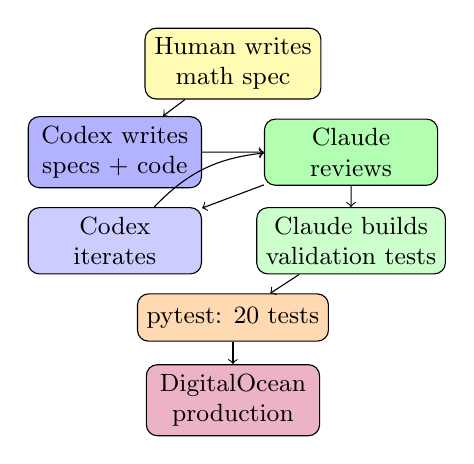
\begin{tikzpicture}[scale=0.75,
    box/.style={rectangle, draw, rounded corners, minimum width=2.2cm, minimum height=0.6cm, align=center, font=\small}]

    \node[box, fill=yellow!30] (human) at (0,4) {Human writes\\math spec};
    \node[box, fill=blue!30] (codex1) at (-2,2.5) {Codex writes\\specs + code};
    \node[box, fill=green!30] (claude1) at (2,2.5) {Claude\\reviews};
    \node[box, fill=blue!20] (codex2) at (-2,1) {Codex\\iterates};
    \node[box, fill=green!20] (claude2) at (2,1) {Claude builds\\validation tests};
    \node[box, fill=orange!30] (pytest) at (0,-0.3) {pytest: 20 tests};
    \node[box, fill=purple!30] (deploy) at (0,-1.7) {DigitalOcean\\production};

    \draw[->] (human) -- (codex1);
    \draw[->] (codex1) -- (claude1);
    \draw[->] (claude1) -- (codex2);
    \draw[->] (claude1) -- (claude2);
    \draw[->] (codex2) to[bend left=20] (claude1);
    \draw[->] (claude2) -- (pytest);
    \draw[->] (pytest) -- (deploy);
\end{tikzpicture}
\end{center}

\textbf{Iteration:} Multiple cycles until all 20 tests pass
\end{frame}

\begin{frame}{Zero-Intervention Automation Pipeline}
\textbf{A Hobby Project with Production-Grade Rigor:}

One prompt triggers the \textbf{entire pipeline} --- no human intervention:

\begin{enumerate}
    \item \textcolor{blue!70}{\textbf{Coding}} --- AI implements from specs
    \item \textcolor{orange!70}{\textbf{Regression Testing}} --- pytest runs 20+ tests locally
    \item \textcolor{purple!70}{\textbf{Browser UI Testing}} --- Playwright validates Flask UI
    \item \textcolor{green!70}{\textbf{Documentation}} --- LaTeX auto-updated
    \item \textcolor{cyan!70}{\textbf{Deploy to DigitalOcean}} --- SSH + Git + systemd
    \item \textcolor{orange!70}{\textbf{Production Regression}} --- Tests on live server
    \item \textcolor{red!70}{\textbf{Telegram Notification}} --- ``Done!''
\end{enumerate}

\vspace{0.2cm}
\begin{center}
\fbox{\parbox{0.85\textwidth}{
\textbf{Key Insight:} \$7/month hobby project built with the same rigor as top tech company production systems.
}}
\end{center}
\end{frame}

\begin{frame}{QuantLib Extension Strategy}
\textbf{QuantLib's Limitations:}
\begin{itemize}
    \item No native callable XCCY support
    \item Limited multi-currency Monte Carlo
    \item No built-in LSM for cross-currency
\end{itemize}

\textbf{How We Extended It (Collaboratively):}
\begin{enumerate}
    \item \textbf{Human:} Defined what QuantLib provides vs what's needed
    \item \textbf{Codex:} Wrote custom Monte Carlo using QuantLib curves
    \item \textbf{Claude:} Verified QuantLib API usage against docs
    \item \textbf{Stack Overflow:} Confirmed edge cases and patterns
\end{enumerate}

\textbf{Result:}
\begin{itemize}
    \item Use QuantLib for: curves, dates, calendars, basic calibration
    \item Custom code for: multi-factor MC, LSM, XCCY cashflows
    \item 1,400+ lines of rigorous extensions
\end{itemize}
\end{frame}

\begin{frame}[fragile]{DigitalOcean Deployment: Detailed Steps}
\textbf{1. Droplet Creation (DigitalOcean Console):}
\begin{itemize}
    \item Region: NYC3 or SFO3 for US users
    \item Image: Ubuntu 22.04 LTS
    \item Plan: Basic \$7/month (2GB RAM, 1 vCPU) --- hobby-friendly!
    \item Authentication: SSH key (not password)
\end{itemize}

\textbf{2. Initial Server Setup:}
\begin{verbatim}
ssh root@your-droplet-ip
apt update && apt upgrade -y
adduser deploy
usermod -aG sudo deploy
\end{verbatim}

\textbf{3. Application Deployment:}
\begin{verbatim}
cd /opt && git clone <repo>
python3 -m venv .venv
.venv/bin/pip install -r requirements.txt
cp deploy/systemd/*.template /etc/systemd/system/
systemctl enable --now tgir-quantlib-tools
\end{verbatim}
\end{frame}

\begin{frame}[fragile]{DigitalOcean: SSL and Apache Configuration}
\textbf{Apache Setup:}
\begin{verbatim}
apt install apache2
a2enmod proxy proxy_http ssl rewrite
cp deploy/apache/*.template /etc/apache2/sites-available/
a2ensite tgir-quantlib-tools
systemctl reload apache2
\end{verbatim}

\textbf{SSL with Certbot:}
\begin{verbatim}
apt install certbot python3-certbot-apache
certbot --apache -d your-domain.com
\end{verbatim}

\textbf{Firewall:}
\begin{verbatim}
ufw allow 22/tcp
ufw allow 80/tcp
ufw allow 443/tcp
ufw enable
\end{verbatim}

\textbf{Result:} HTTPS-secured Flask app at \texttt{https://your-domain.com}
\end{frame}

\begin{frame}{Why Codex + Claude Collaboration Works}
\textbf{Complementary Strengths:}
\begin{itemize}
    \item \textbf{Codex:} Excellent at ground-up implementation from specs
    \item \textbf{Claude:} Excellent at review, validation, extension
    \item \textbf{Human:} Domain expertise, orchestration, final judgment
\end{itemize}

\textbf{Error Detection:}
\begin{itemize}
    \item Claude catches bugs in Codex's implementations
    \item Codex fixes issues Claude identifies
    \item Neither alone would produce same quality
\end{itemize}

\textbf{Stack Overflow Role:}
\begin{itemize}
    \item AI can hallucinate APIs that don't exist
    \item Human experts catch edge cases
    \item Community validates approaches
\end{itemize}

\textbf{Key Lesson:}\\[0.2cm]
\fbox{\parbox{0.85\textwidth}{\centering Two AI agents + human domain expert\\produces better results than any single agent}}
\end{frame}

\begin{frame}{The Methodology IS the Innovation}
\textbf{This project delivers TWO things:}

\begin{enumerate}
    \item \textbf{Callable XCCY Pricer:}
    \begin{itemize}
        \item Three-factor Monte Carlo
        \item Longstaff-Schwartz optimization
        \item 20 validation tests
        \item Production deployment
    \end{itemize}

    \item \textbf{Collaborative Development Methodology:}
    \begin{itemize}
        \item Human $\to$ Codex (specs, implementation)
        \item Codex $\to$ Claude (review, validation)
        \item Claude $\to$ Regression tests (future-proofing)
        \item Full ecosystem: Mac + DigitalOcean + QuantLib + Python
    \end{itemize}
\end{enumerate}

\vspace{0.3cm}
\textbf{The methodology is reusable for other complex pricers}

\fbox{\parbox{0.85\textwidth}{\centering The collaborative workflow is as valuable as the callable XCCY pricer itself}}
\end{frame}

\begin{frame}{Reusable Human-Agent Development Pattern}
\begin{center}
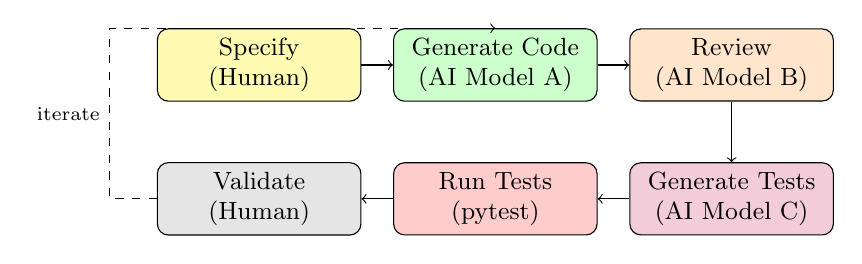
\begin{tikzpicture}[
    box/.style={rectangle, draw, rounded corners, text width=2.35cm, minimum height=0.9cm, align=center, font=\small}]
    \node[box, fill=yellow!30] (spec) at (-3,2.4) {Specify\\(Human)};
    \node[box, fill=green!20] (gen) at (0,2.4) {Generate Code\\(AI Model A)};
    \node[box, fill=orange!20] (review) at (3,2.4) {Review\\(AI Model B)};
    \node[box, fill=purple!20] (test) at (3,0.7) {Generate Tests\\(AI Model C)};
    \node[box, fill=red!20] (run) at (0,0.7) {Run Tests\\(pytest)};
    \node[box, fill=gray!20] (valid) at (-3,0.7) {Validate\\(Human)};

    \draw[->] (spec) -- (gen);
    \draw[->] (gen) -- (review);
    \draw[->] (review) -- (test);
    \draw[->] (test) -- (run);
    \draw[->] (run) -- (valid);
    \draw[->, dashed] (valid.west) -- ++(-0.6,0) |- node[pos=0.25,left,font=\scriptsize] {iterate} (gen.north);
\end{tikzpicture}
\end{center}

\textbf{Key Principle:}\\[0.3cm]
\fbox{\parbox{0.85\textwidth}{\centering Human provides specifications and validation\\AI accelerates implementation and review}}
\end{frame}

\begin{frame}{}
\begin{center}
\Huge\textbf{End of Supplementary Material}\\[2cm]
\Large Return to Main Presentation
\end{center}
\end{frame}

\end{document}
